\chapter{VDP Range Selection}\label{chapter:parameter-range-selection}

Ensuring that the ranges for each \gls{vdp} are realistic and representative is critical in accurately quantifying the relative influence of each \gls{vdp}. Overestimating a \gls{vdp} range will overestimate its relative influence and vica versa underestimating a \gls{vdp} range would underestimate its relative influence. The rationale for selecting the ranges for each \gls{vdp} is presented in the sections that follow.

%==============================================
%      SECTION
%==============================================
\section{Geometric Parameter Limits}\label{section:geometric-limits}

The \gls{pbs} scheme is still in the pilot project stages in South Africa and as part of the pilot project the vehicles that form part of the \gls{pbs} fleet still need to adhere to certain regulations as stipulated within the \gls{nrta} unless special permission is given by the \gls{ndot} in the form of a operational approval.

The \gls{pbs} scheme is designed to develop safer, more productive \glspl{hcv} without the requirement of being governed by a prescriptive framework. Kienh{\"o}fer et al. \cite{Kienhofer2014} evaluated the \gls{mod} and \gls{dom} performance and highlighted that the prescriptive framework allows for the most lenient geometrical constraints for frontal overhang when compared to Australia, the European Union, Canada, and the United States. Thus, the prescriptive framework was used as a guide to determine the maximum dimensional limits for each combination while simultaneously ensuring that the geometry would be structurally possible with the baseline design. The prescriptive legislation for maximum vehicle dimensions in South Africa is detailed in Part III of the \gls{nrta} (Act No. 93 of 1996) \cite{NationalDepartmentofTransport2003} and any regulation numbers included in the tables below refer to this document.

The vehicle geometry plays the largest role in the low-speed performance (\gls{lssp}, \gls{fs}, \gls{ts}, \gls{mod}, \gls{dom}). The geometrical reference points used to calculate these are described in the \gls{pbs} scheme \cite{NationalTransportCommission2008} as follows:

\begin{enumerate}
	\item \textbf{Forward reference points:} \enquote{the vertical projection of the furthest forward or outside point, or points, on the vehicle}
	\item \textbf{Rear reference points:} \enquote{the vertical projection of the furthest rearward or outside point, or points, on the vehicle}
\end{enumerate}

Minimum dimensional limits are not explicitly defined in the \gls{nrta} and have been determined according to either physical constraints or other limitations which will be discussed in the sections that follow.

%      SUBSECTION
%----------------------------------------------
\subsection{Front Overhang}\label{section:pr-frontal-overhang}

A representative frontal overhang for the prime movers was determined from \gls{oem} catalogues, the data from which is included in Table~\ref{table:oem-front-overhang}.

%----------------------------------------------
%      TABLE
%----------------------------------------------
\begin{table}[H]
	\centering\footnotesize
	\begin{threeparttable}

		\begin{tabulary}{\textwidth}{lc}
			\toprule
			\textbf{Prime mover model} & \textbf{Front overhang (mm)} \\
			\midrule
			Volvo FH42T3LA \cite{VolvoTruckCorporation2017FH42T3LA} & 1365 \\
			Mercedes Benz Atego \cite{MercedesBenzAtego2015} & 1380 \\
			Scania G440/480 8x4 \cite{ScaniaG4404806x4} & 1455 \\
			DAF FTT XF105.460 \cite{DAFXF105.4602017} & 1370 \\
			Volvo FM64T3HBX \cite{VolvoTruckCorporation2018FM64T3HBX} & 1520 \\
			\bottomrule
		\end{tabulary}

		\caption{OEM prime mover front overhangs\tnote{1}}
		\label{table:oem-front-overhang}

		\begin{tablenotes}
			\item[1] SAE up co-ordinate system and origin taken from centre of steer axle or hitch point (for trailers) at ground level
		\end{tablenotes}

	\end{threeparttable}
\end{table}
%----------------------------------------------
%      TABLE
%----------------------------------------------

Regulation 221 in the \gls{nrta} allows for a 300 mm projection forward of the front of cab for a bull-bar and therefore considering a worst case frontal cab overhang of 1520~mm, the maximum overhang with a bull-bar will be considered 300~mm ahead of this at the same width of the cab.

The front overhang in the case of the trailer units and rigid truck were limited according to regulation 226 (1)(a) which allows a frontal overhang of up to 1800~mm for a semi-trailer.  The swing radius of all the models were checked to ensure that there would be no collision with the unit ahead of it. The limit was set such that there would be a 50 mm clearance between the leading unit and the swing radius of the following unit.

In the case of the tridem interlink follower, the baseline frontal overhang is negative (behind the hitch) which was used as the minimum. All other trailer frontal overhangs were evaluated as 0~mm from the hitch connection assuming a narrow chassis section extends further to structurally support the 5th wheel hitch connection.

The resulting parameter range for the front overhangs of each unit is provided in Table~\ref{table:parameter-range-front-overhang}.

%----------------------------------------------
%      TABLE - UPDATED TO NEW RANGES
%----------------------------------------------
\begin{table}[H]
	\centering\footnotesize
	\begin{threeparttable}

		\begin{tabulary}{\textwidth}{lcccll}
			\toprule
			\textbf{Vehicle unit} & \textbf{Baseline (mm)} & \textbf{Min. (mm)} & \textbf{Max. (mm)} & \textbf{Rationale min.} & \textbf{Rationale max.} \\
			\midrule
            Truck tractor & 1365  & 1300  & 1820  & OEM variations & OEM variations \\
            Rigid truck & 1365  & 1300  & 1820  & OEM variations & OEM variations \\
            Quad semi-trailer & 900   & 0     & 1800  & Structural & Regulation 226 (a) \\
            Tridem interlink leader & 950   & 0     & 1800  & Structural & Regulation 226 (a) \\
            Tridem interlink follower & -354  & -354  & 464   & Structural & Structural \\
            Tridem semi-trailer & 1760  & 0     & 1800  & Structural & Regulation 226 (a) \\
			\bottomrule
		\end{tabulary}

		\caption{Parameter range - front overhang\tnote{1}}
		\label{table:parameter-range-front-overhang}

		\begin{tablenotes}
			\item[1] SAE up co-ordinate system and origin taken from centre of steer axle or hitch point (for trailers) at ground level
		\end{tablenotes}

	\end{threeparttable}
\end{table}
%----------------------------------------------
%      TABLE
%----------------------------------------------

%      SUBSECTION
%----------------------------------------------
\subsection{Rear Overhang}\label{section:pr-rear-overhang}

All rear overhangs were considered at the point where the structure of the unit was at its widest. Narrow chassis extensions were ignored.

Regulation 226 (2)(c) states that the maximum rear overhang of any semi-trailer or other vehicle (other than refuse collectors, road making, road construction, farming  vehicles and vehicles with a single axle or axle unit) may not exceed 60 \% of the wheelbase measured from the centre of the rearmost axle on the unit. This was considered along with structural constraints to develop the maximum rear overhang reference points.

The reference point evaluated for the rear overhang of the 6x4 truck-tractor is at the furthest rear and widest point on the wheel arch. Further past this, the chassis extension is narrow and is not used as a reference point in the manoeuvres. As a result, the rear overhang was not evaluated for this vehicle unit.

In the case of the rigid truck, the superstructure could legally extend further back to the NRTA limit of 60\% of the wheelbase. This would cause the rigid payload to extend into the rear semi-trailer. Considering the swing radius of the rear trailer of 2188 mm, the maximum rear overhang of the rigid payload with a 50 mm clearance to ensure no contact in dynamic manoeuvres would be 2546 mm from the rear axle as can be seen in Figure~\ref{figure:parameter-selection-rear-overhang-of-rigid-truck}

%----------------------------------------------
%      FIGURE
%----------------------------------------------
\begin{figure}[H]
	\centering
	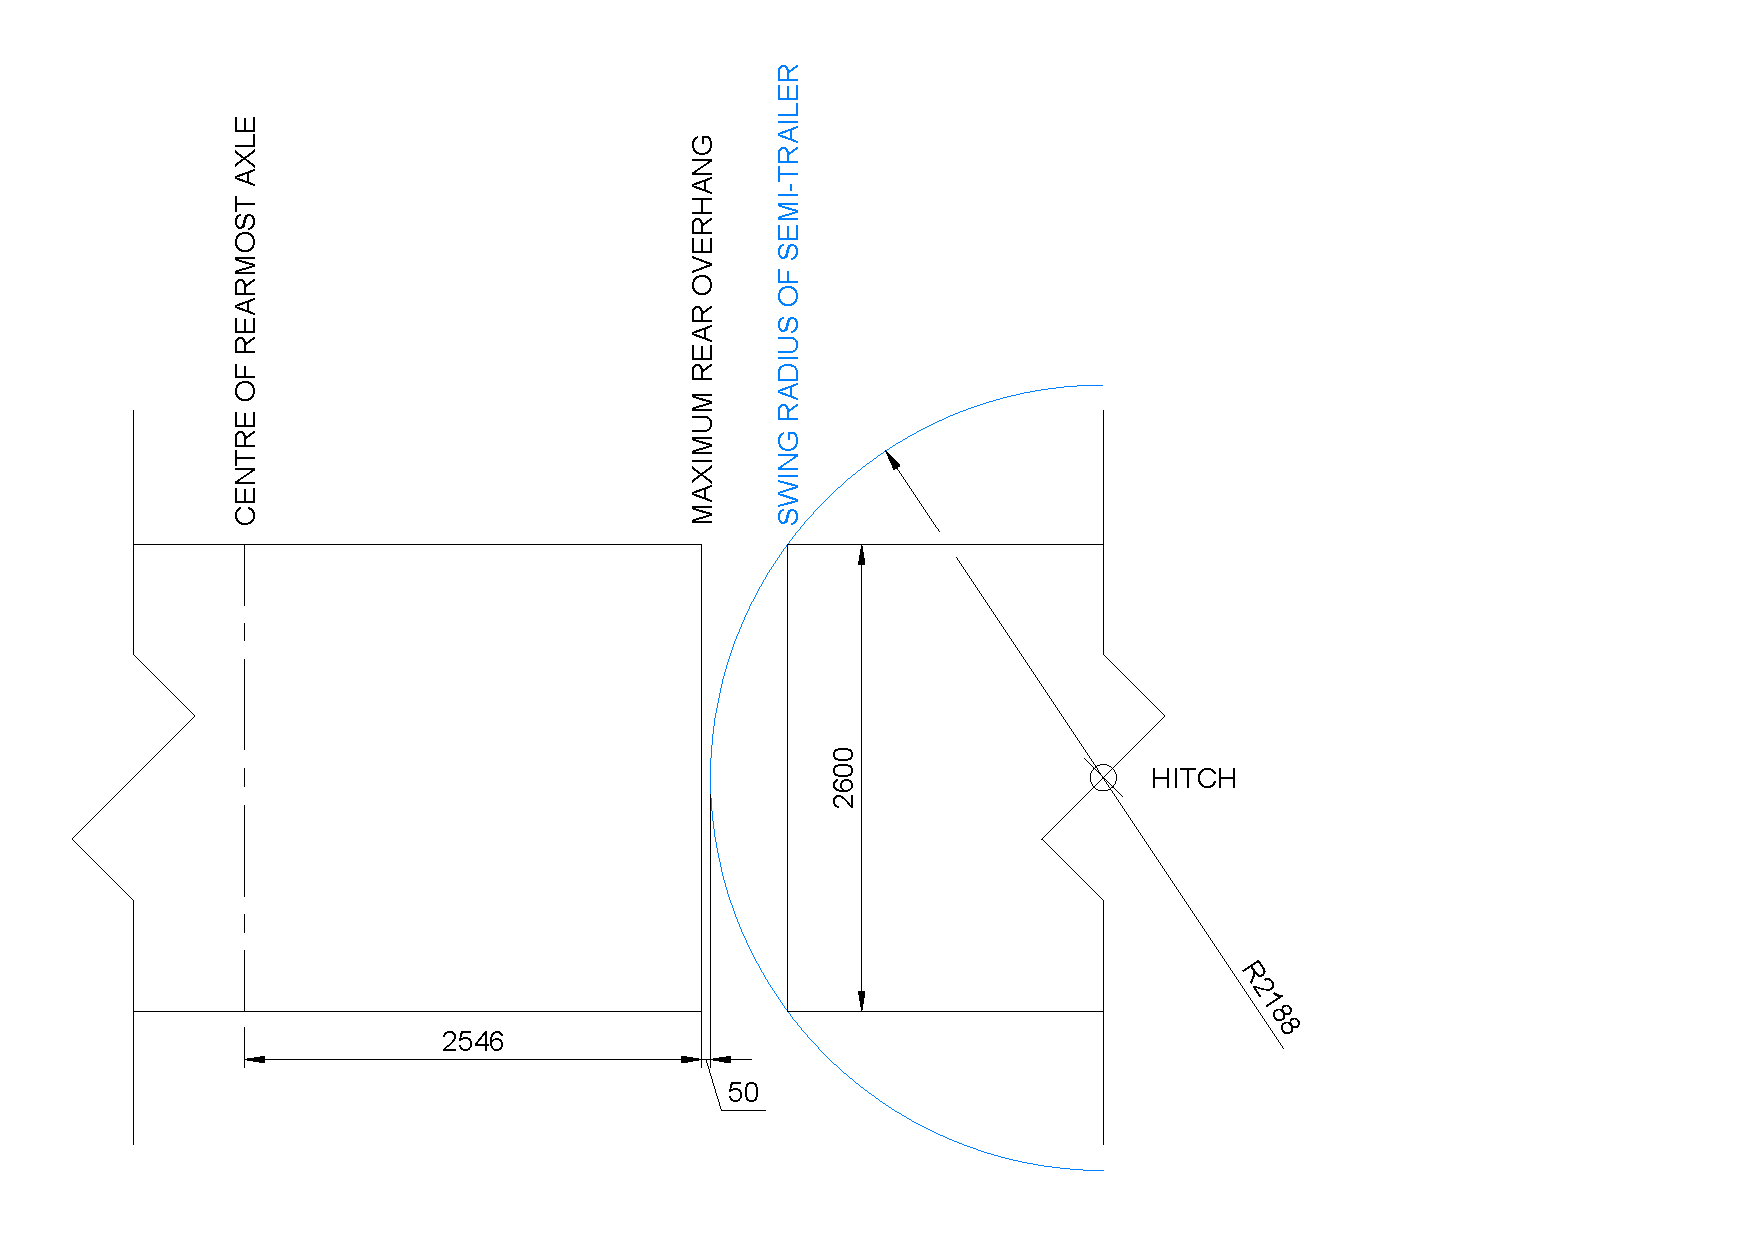
\includegraphics[width=1\textwidth]{fig/parameter-selection_rear-overhang_rigid-truck}
	\caption{Rear overhang of the rigid truck}
	\label{figure:parameter-selection-rear-overhang-of-rigid-truck}
\end{figure}
%----------------------------------------------
%      FIGURE
%----------------------------------------------

Similarly, the maximum rear overhang for the tridem interlink leader was determined geometrically from the swing radius of the narrow follower chassis as shown in Figure~\ref{figure:parameter-selection-rear-overhang-of-b-double-leader}.

%----------------------------------------------
%      FIGURE
%----------------------------------------------
\begin{figure}[H]
	\centering
	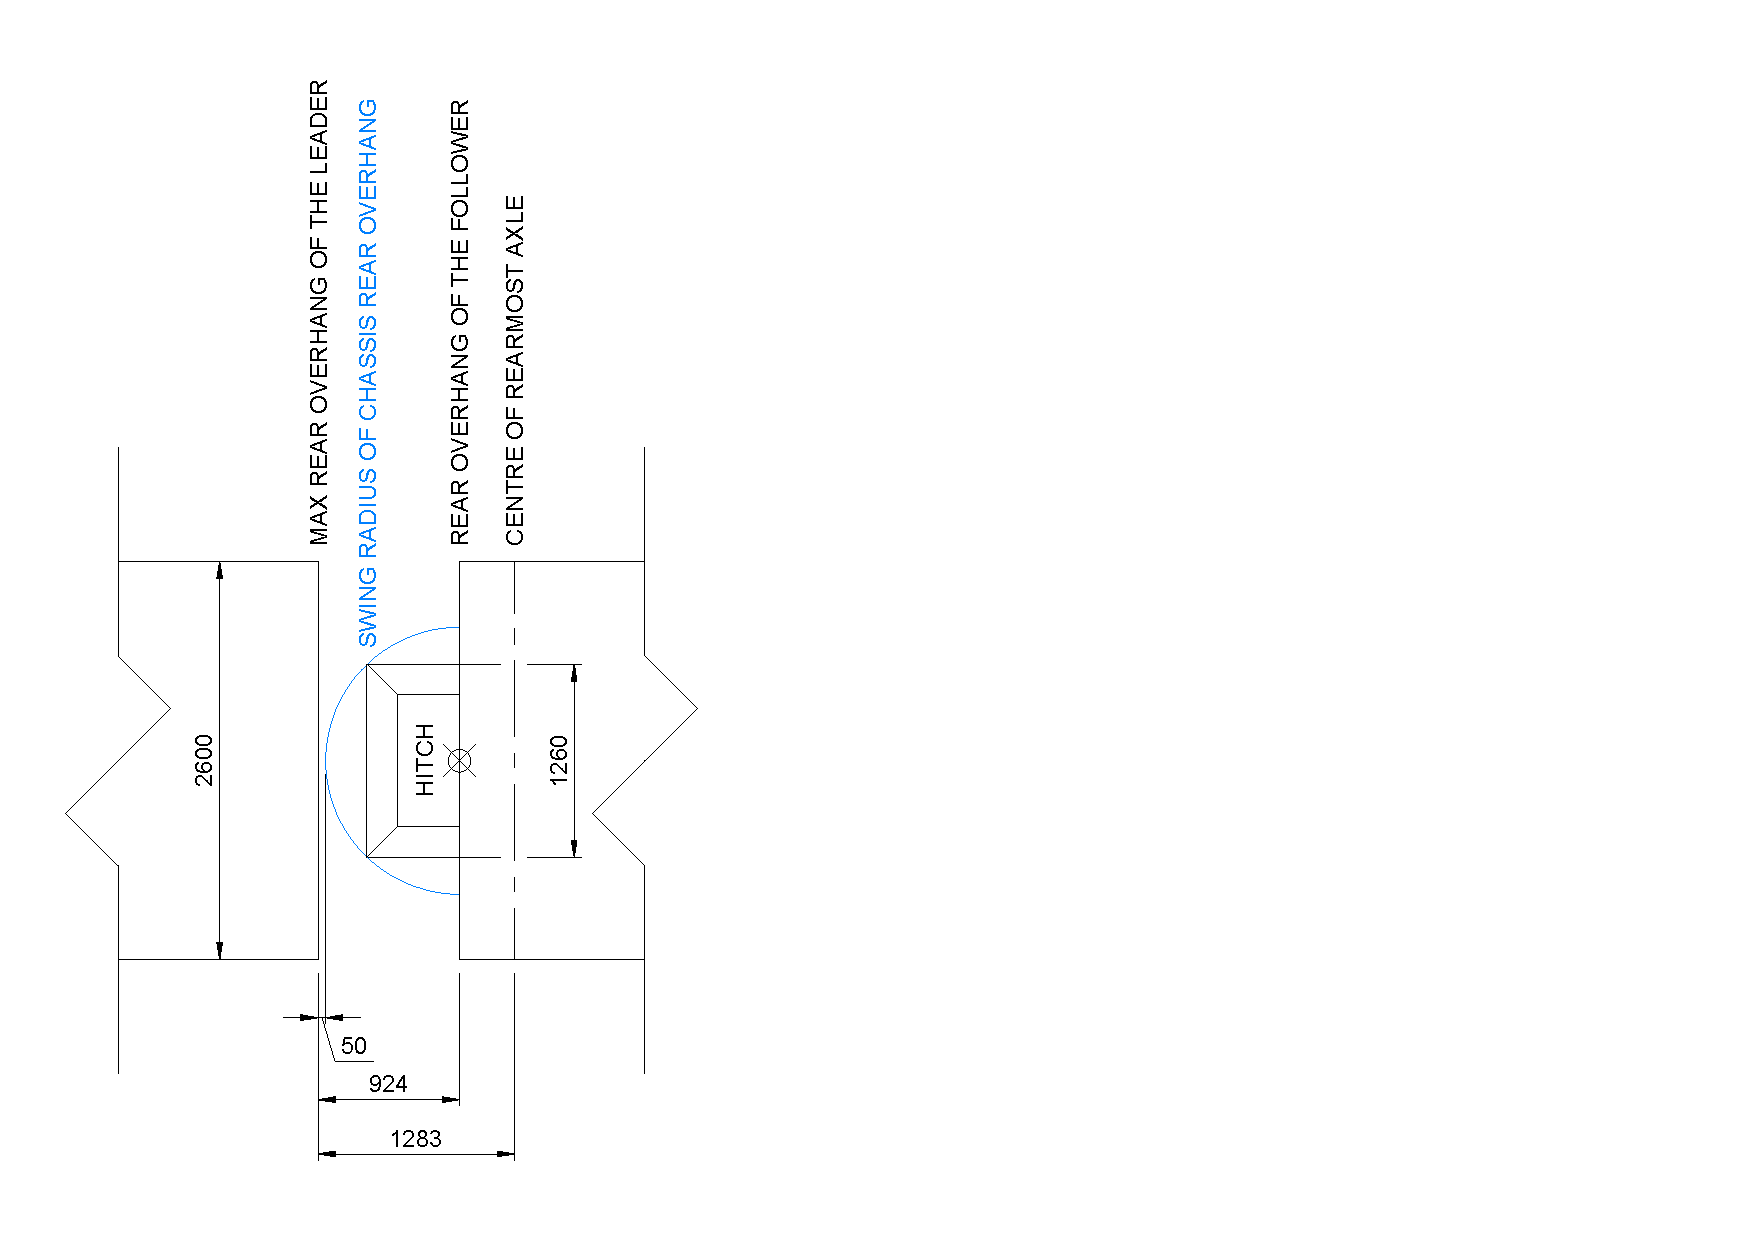
\includegraphics[width=0.7\textwidth]{fig/parameter-selection_rear-overhang_b-double-leader}
	\caption{Rear overhang of the tridem interlink leader trailer}
	\label{figure:parameter-selection-rear-overhang-of-b-double-leader}
\end{figure}
%----------------------------------------------
%      FIGURE
%----------------------------------------------

The resulting range of rear overhangs is summarised in Table~\ref{table:parameter-range-rear-overhang}.

%----------------------------------------------
%      TABLE - UPDATED TO NEW RANGES
%----------------------------------------------
\begin{table}[H]
	\centering\footnotesize
	\begin{threeparttable}

		\begin{tabulary}{\textwidth}{lcccll}
			\toprule
			\textbf{Vehicle unit} & \textbf{Baseline (mm)} & \textbf{Min. (mm)} & \textbf{Max. (mm)} & \textbf{Rationale min.} & \textbf{Rationale max.} \\
			\midrule
            Truck tractor & 1013  & 1013  & 1013  & No impact & No impact \\
            Rigid truck & 1775  & 0     & 2546  & Assumption & Structural \\
            Quad semi-trailer & 1960  & 0     & 6000  & Assumption & Regulation 226 (2)(c) \\
            Tridem interlink leader & -1790 & -1790 & -1283 & Structural & Structural \\
            Tridem interlink follower & 984   & 0     & 3570  & Assumption & Structural \\
            Tridem semi-trailer & 1081  & 0     & 4953  & Assumption & Regulation 226 (2)(c) \\
			\bottomrule
		\end{tabulary}

		\caption{Parameter range - rear overhang \tnote{1}}
		\label{table:parameter-range-rear-overhang}

		\begin{tablenotes}
			\item[1] Measured from the centre of the rearmost axle in accordance with Regulation 226 (2)(c)
		\end{tablenotes}

	\end{threeparttable}
\end{table}
%----------------------------------------------
%      TABLE
%----------------------------------------------

%      SUBSECTION
%----------------------------------------------
\subsection{Vehicle Width}\label{section:pr-vehicle-width}

The maximum width for all vehicle units was assumed to be the legal maximum of 2600~mm.

The minimum vehicle width for the prime mover was determined from overall widths provided in \gls{oem} datasheets as summarised in Table~\ref{table:parameter-selection-oem-prime-mover-widths}.

%----------------------------------------------
%      TABLE
%----------------------------------------------
\begin{table}[H]
	\centering\footnotesize
	\begin{threeparttable}

		\begin{tabulary}{\textwidth}{lc}
			\toprule
			\textbf{Prime Mover Model} & \textbf{Overall width (mm)} \\
			\midrule
			Volvo FM64T3HBX \cite{VolvoTruckCorporation2018FM64T3HBX} & 2490 \\
			Mercedes Benz Atego 1528 LS-36 \cite{MercedesBenzAtego2015} & 2228 \\
			DAF FTT XF105.460 \cite{DAFXF105.4602017} & 2540 \\
			\bottomrule
		\end{tabulary}

		\caption{Selection of \gls{oem} prime mover widths}
		\label{table:parameter-selection-oem-prime-mover-widths}

		% 		\begin{tablenotes}
		% 			\item[1] %\tnote{1}
		% 		\end{tablenotes}

	\end{threeparttable}
\end{table}
%----------------------------------------------
%      TABLE
%----------------------------------------------

The reference points used for the low-speed standards on the front of a cab are generally narrower than maximum vehicle width due to the curvature of the bumper. As a result, the width of the reference points (furthest forward or outside) used for the minimum and maximum vehicle width were determined as listed with an illustration following in Figure~\ref{figure:parameter-selection-vehicle-width}:

\begin{enumerate}
	\item The maximum width at 2600~mm with a 100 mm radius corner, at a 30\degree{} angle anti-clockwise to the transverse axis \footnote{The low-speed performance of a combination is determined by the selected reference point on the vehicle. A reference point located further forward of the steer axle or outward of the vehicle centreline will result in greater road-width usage. When locating a reference point on a radius, using a more forward location will not necessarily indicate worse performance since the point will be located further inward towards the vehicle centreline. A 30\degree{} angle from the transverse axis has been found in practice to yield approximate worst-case evaluation of low-speed performance within a suitable accuracy and has become the standard method at Wits in evaluating the performance of a combination where reference points reside on a radius such as the payload of a car-carrier.}
	\item The minimum width at 2200~mm with a 500 mm radius corner, at a 30\degree{} angle anti-clockwise to the transverse axis
\end{enumerate}

%----------------------------------------------
%      FIGURE
%----------------------------------------------
\begin{figure}[H]
	\centering
	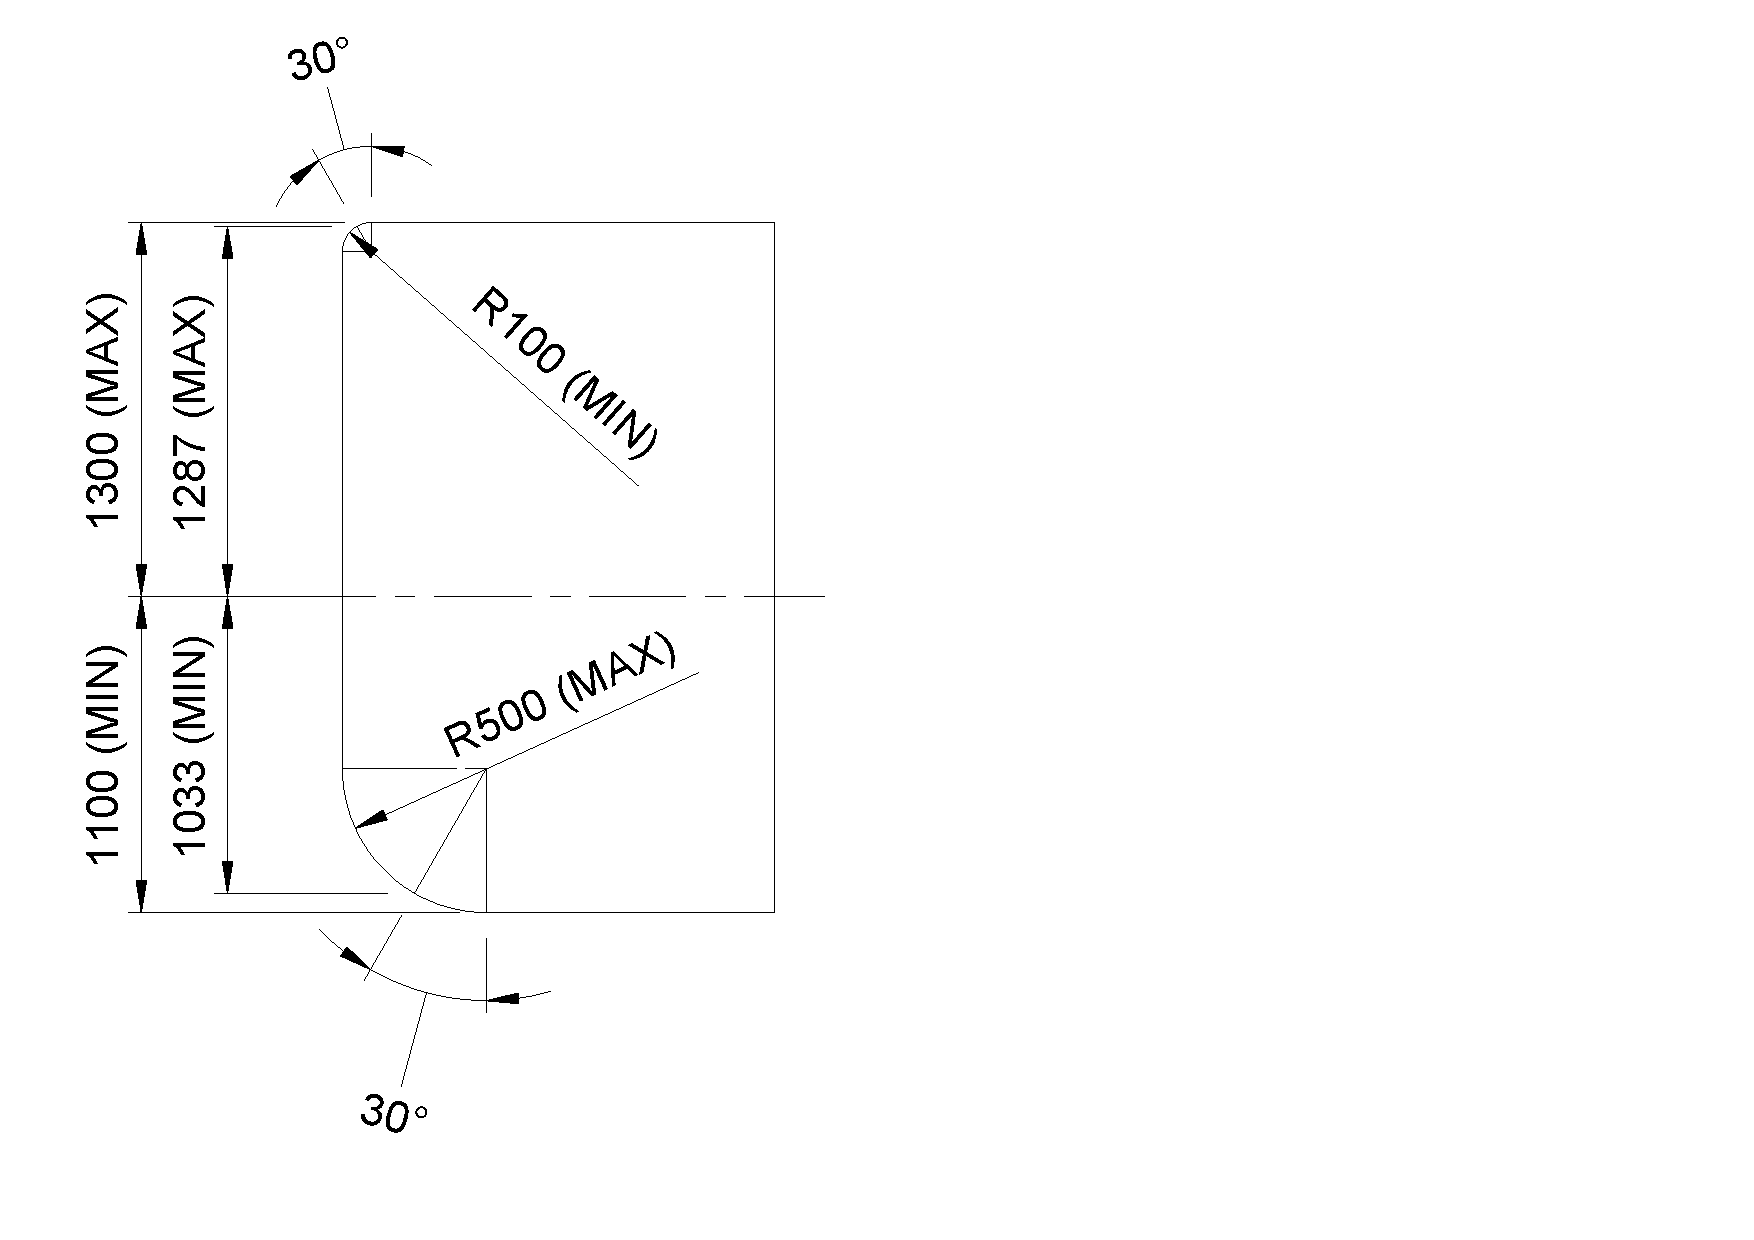
\includegraphics[width=0.5\textwidth]{fig/parameter-selection_vehicle-width_prime-mover}
	\caption{Parameter selection - prime mover frontal reference points}
	\label{figure:parameter-selection-vehicle-width}
\end{figure}
%----------------------------------------------
%      FIGURE
%----------------------------------------------

The trailer units were modelled as boxes without any curvature. The minimum width for a trailer was assumed to be 2400~mm, beyond which the deck width would become too small and unproductive.

A summary of the vehicle widths for all units is provided in Table~\ref{table:pr-vehicle-width}.

%----------------------------------------------
%      TABLE
%----------------------------------------------
\begin{table}[H]
	\centering\footnotesize
	\begin{threeparttable}

		\begin{tabulary}{\textwidth}{lccc}
			\toprule
			\textbf{Vehicle unit} & \textbf{Baseline (mm)} & \textbf{Min. (mm)} & \textbf{Max. (mm)} \\
			\midrule
			Prime mover (all) & 2495  & 2225  & 2600 \\
			Trailer (all) & 2600  & 2400  & 2600 \\
			\bottomrule
		\end{tabulary}

		\caption{Parameter range - vehicle width}
		\label{table:pr-vehicle-width}

		% 		\begin{tablenotes}
		% 			\item[1] %\tnote{1}
		% 		\end{tablenotes}

	\end{threeparttable}
\end{table}
%----------------------------------------------
%      TABLE
%----------------------------------------------

\subsection{Reference Point Height}\label{section-pr-ref-point-height}

Geometrical reference points at the forward-most outer and rearward-most outer of a \gls{hcv} are used to evaluating the amount of road space that a \gls{hcv} requires when performing road manoeuvres. The NTC rules \cite{NationalTransportCommission2008} state that if multiple points reside at the same reference point, the lowest of those points should be used.

The reference point height can range from ground height (for example a mud flap or sidewalls of a tyre) up to 4600~mm in the case of a car-carrier which is allowed an overall height of 4600~mm if approved as a \gls{pbs} safe vehicle \cite{AbnormalLoadTechnicalCommittee2014}. Thus, to encompass the worst case for all \glspl{hcv}, the reference points on each vehicle unit were varied from 0~mm to 4600~mm.

%      SUBSECTION
%----------------------------------------------
\subsection{Prime Mover and Trailer Wheelbase}\label{section:pr-wheelbase}

The range of wheelbases selected for each vehicle unit was determined using structural limitations in conjunction with Regulation 225 (b) regulating the maximum wheelbase for a vehicle unit and the previously mentioned Regulation 226 (2)(c) regulating the maximum rear overhang from the centre of the rearmost axle (see Section~\ref{section:pr-rear-overhang}).

Changing the wheelbase has a significant effect on the axle loadings and the baseline vehicles are based on PBS vehicles with axle loadings close to the legal limits. If the wheelbase were to be varied within a range where the axle loads remained legal, there would be minimal variation. This would remove insight into how the wheelbase impacts vehicle performance in the case of volume limited transport where the axle loadings have more scope to vary. Thus, for the selection of wheelbases, legal axle load requirements were ignored.

The minimum wheelbase was selected according to the following conditions:

\begin{enumerate}
	\item The resulting rear overhang reached 60\% of the wheelbase
	\item The hitch location coincides with the centre of the rearmost axle
	\item The vehicle configuration becomes unstable \footnote{Since the wheelbases are varied over a large range without altering the location of the payload, the vehicle model became unstable for short wheelbases. In these cases, the minimum wheelbase was increased in increments of 50~mm until the model became stable.}
\end{enumerate}

The maximum wheelbase was selected according to the following conditions:

\begin{enumerate}
	\item The maximum wheelbase for a semi-trailer of 10~m according to Regulation 225 (b)
	\item The edge of the tyre aligns with the edge of the chassis structure
	\item The edge of the tyre aligns with the pintle hitch connection point
\end{enumerate}

The maximum and minimum wheelbases are illustrated in Figures~\ref{figure:parameter-selection-wheelbase-quad-semi-trailer}~to~\ref{figure:parameter-selection-wheelbase-truck-and-dog}.

%----------------------------------------------
%      FIGURE
%----------------------------------------------
\begin{figure*}[!htbp]
	\centering
	\begin{subfigure}[t]{1\textwidth}
		\centering
		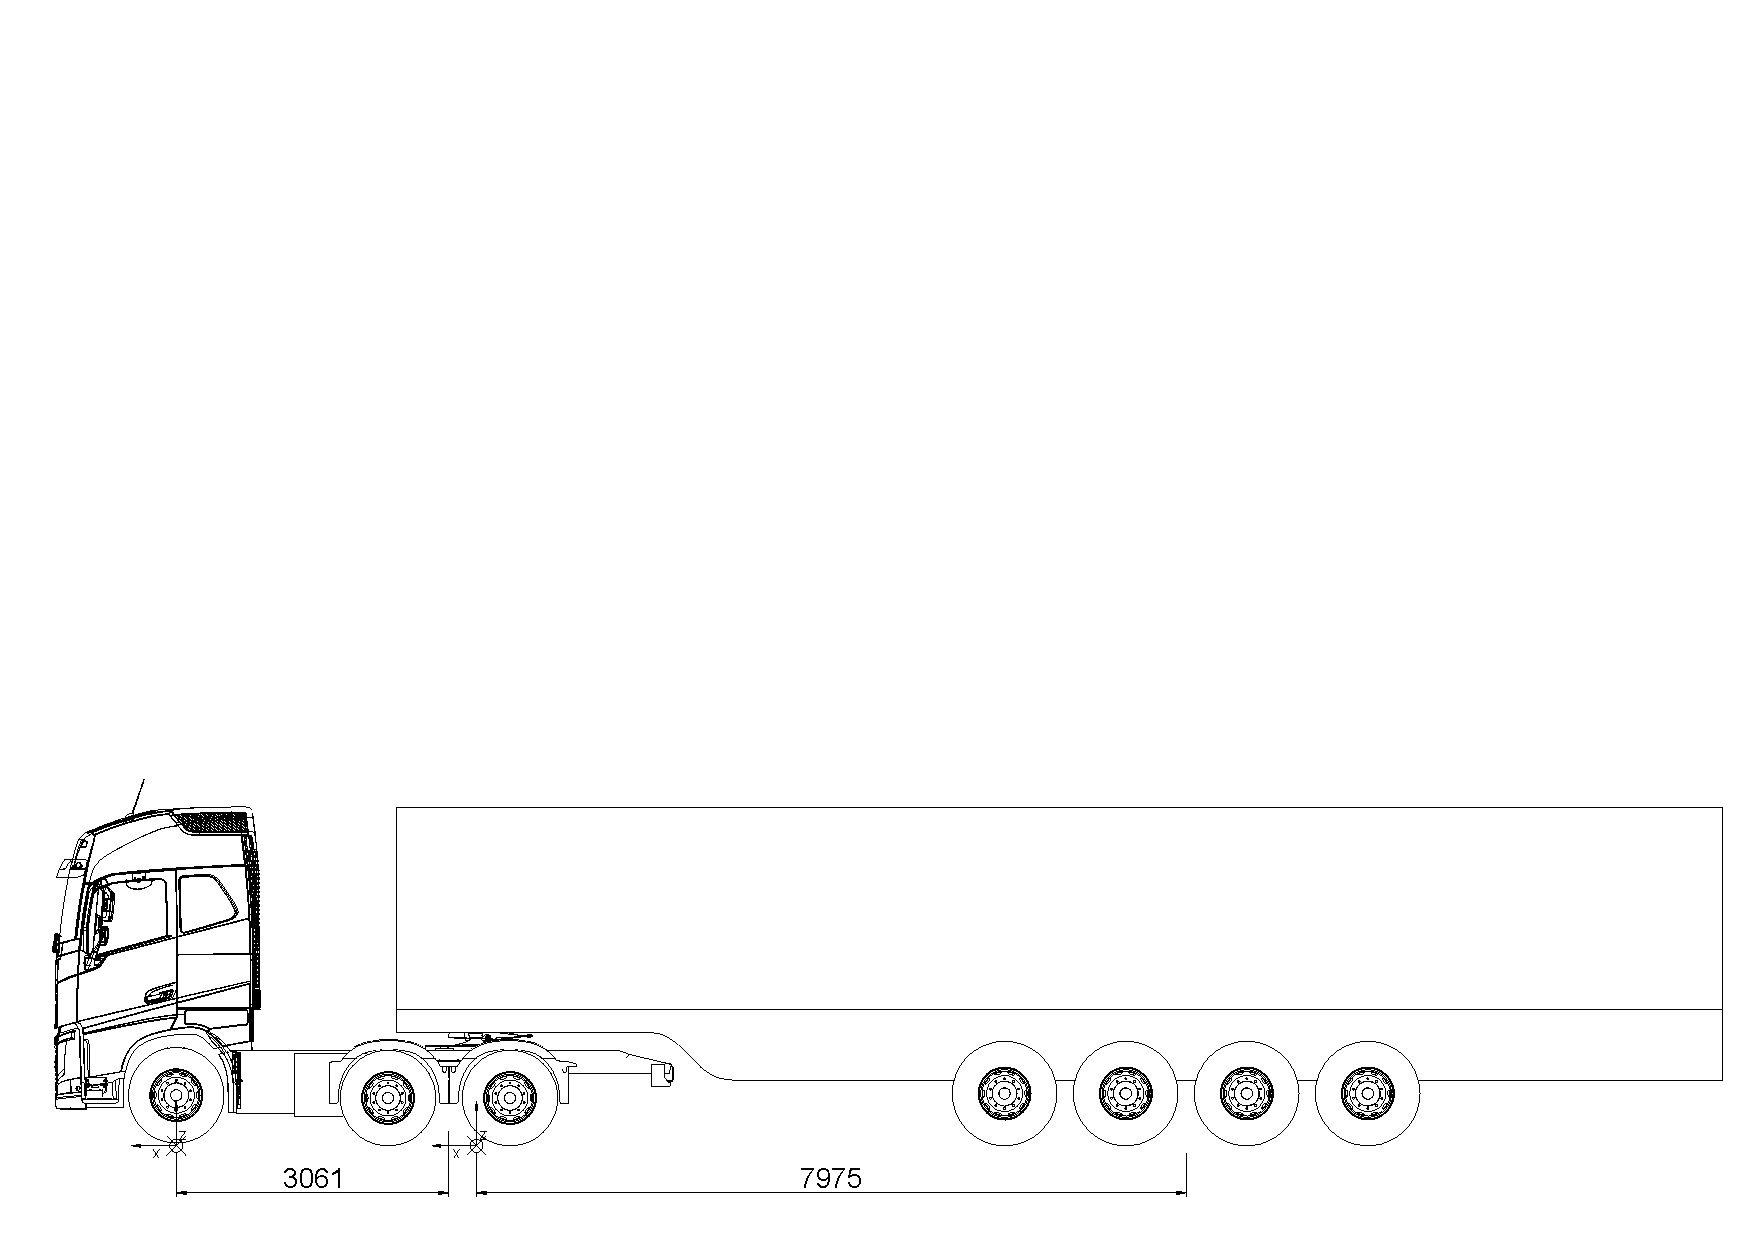
\includegraphics[width=1\textwidth]{fig/parameter-selection_wheelbase_min_quad-semi-trailer}
		\caption{Minimum wheelbase}
	\end{subfigure}%

	\begin{subfigure}[t]{1\textwidth}
		\centering
		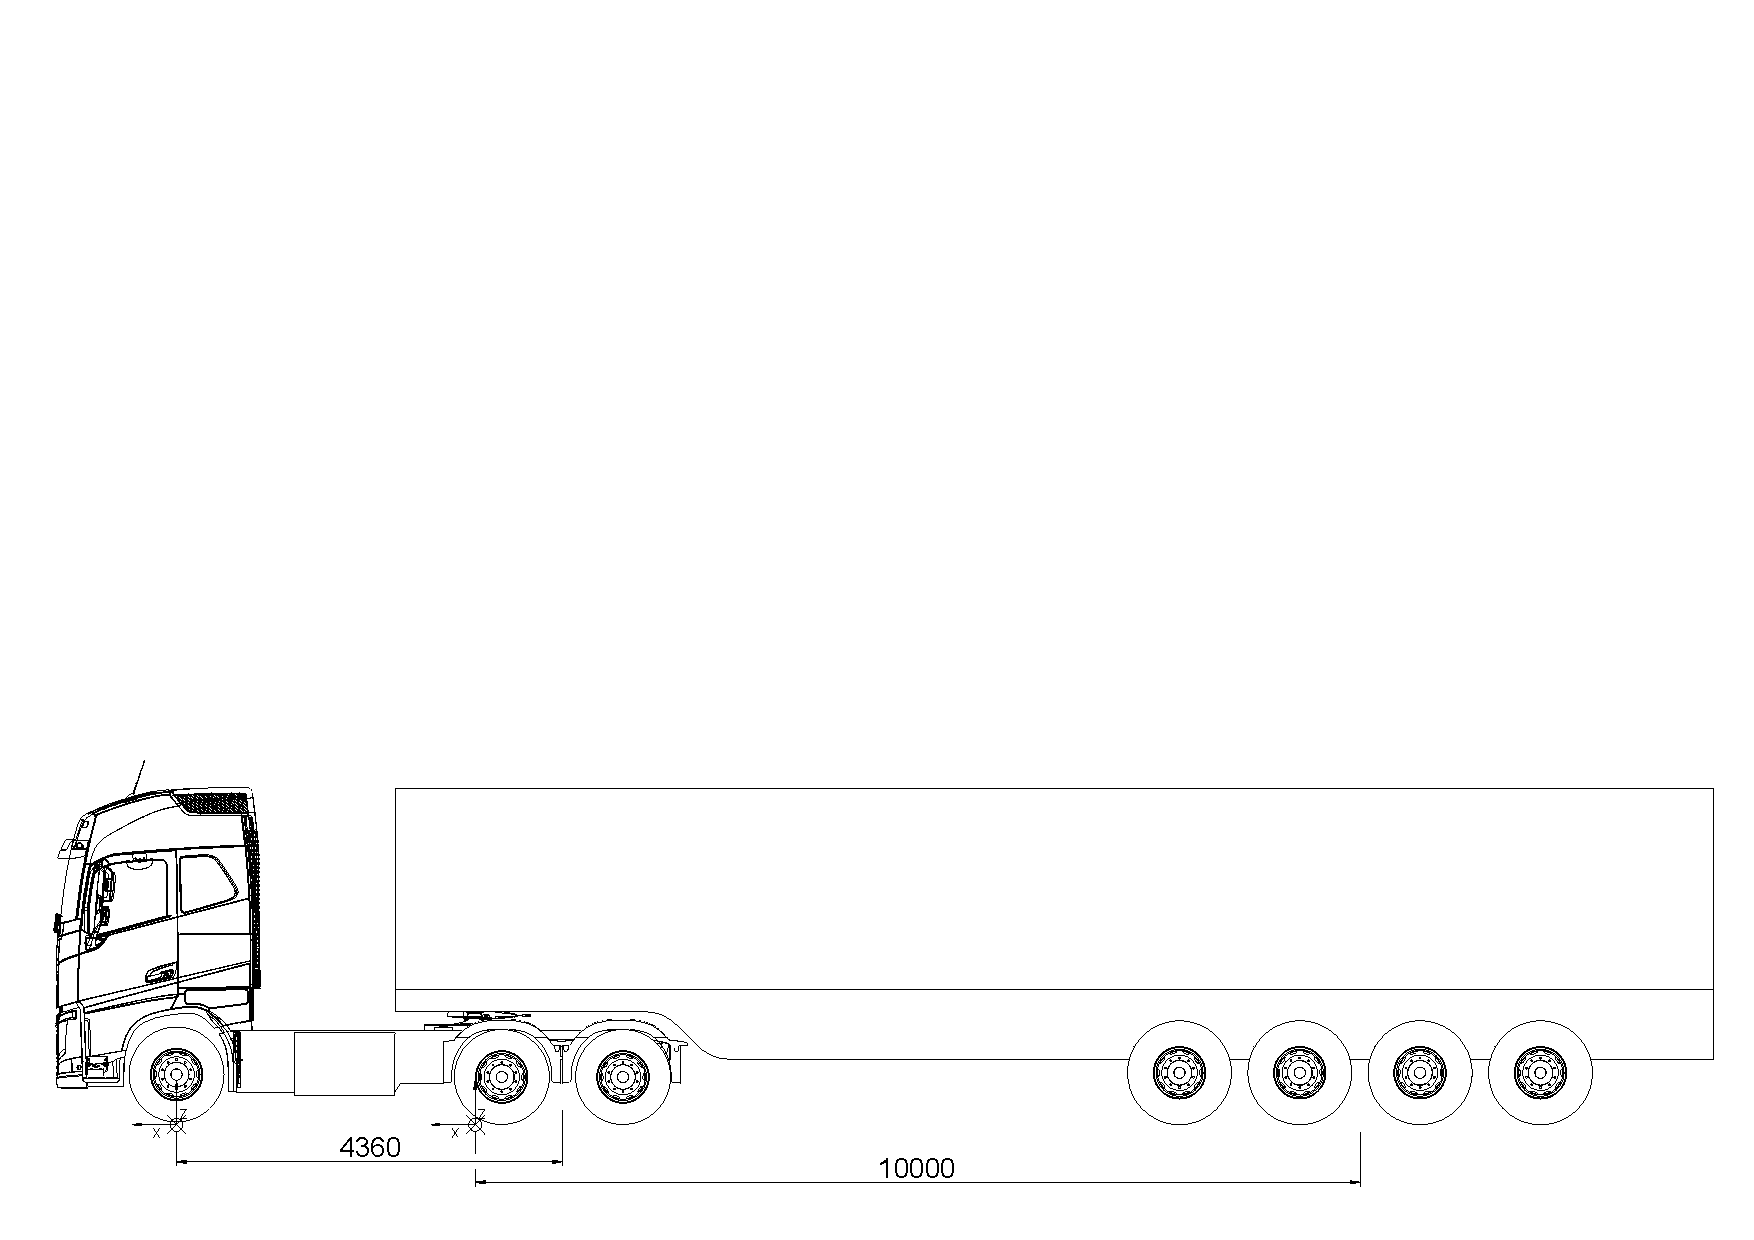
\includegraphics[width=1\textwidth]{fig/parameter-selection_wheelbase_max_quad-semi-trailer}
		\caption{Maximum wheelbase}
	\end{subfigure}

	\caption{Parameter selection - wheelbases for the quad semi-trailer combination}
	\label{figure:parameter-selection-wheelbase-quad-semi-trailer}
\end{figure*}
%----------------------------------------------
%      FIGURE
%----------------------------------------------

%----------------------------------------------
%      FIGURE
%----------------------------------------------
\begin{figure*}[!htbp]
	\centering
	\begin{subfigure}[t]{1\textwidth}
		\centering
		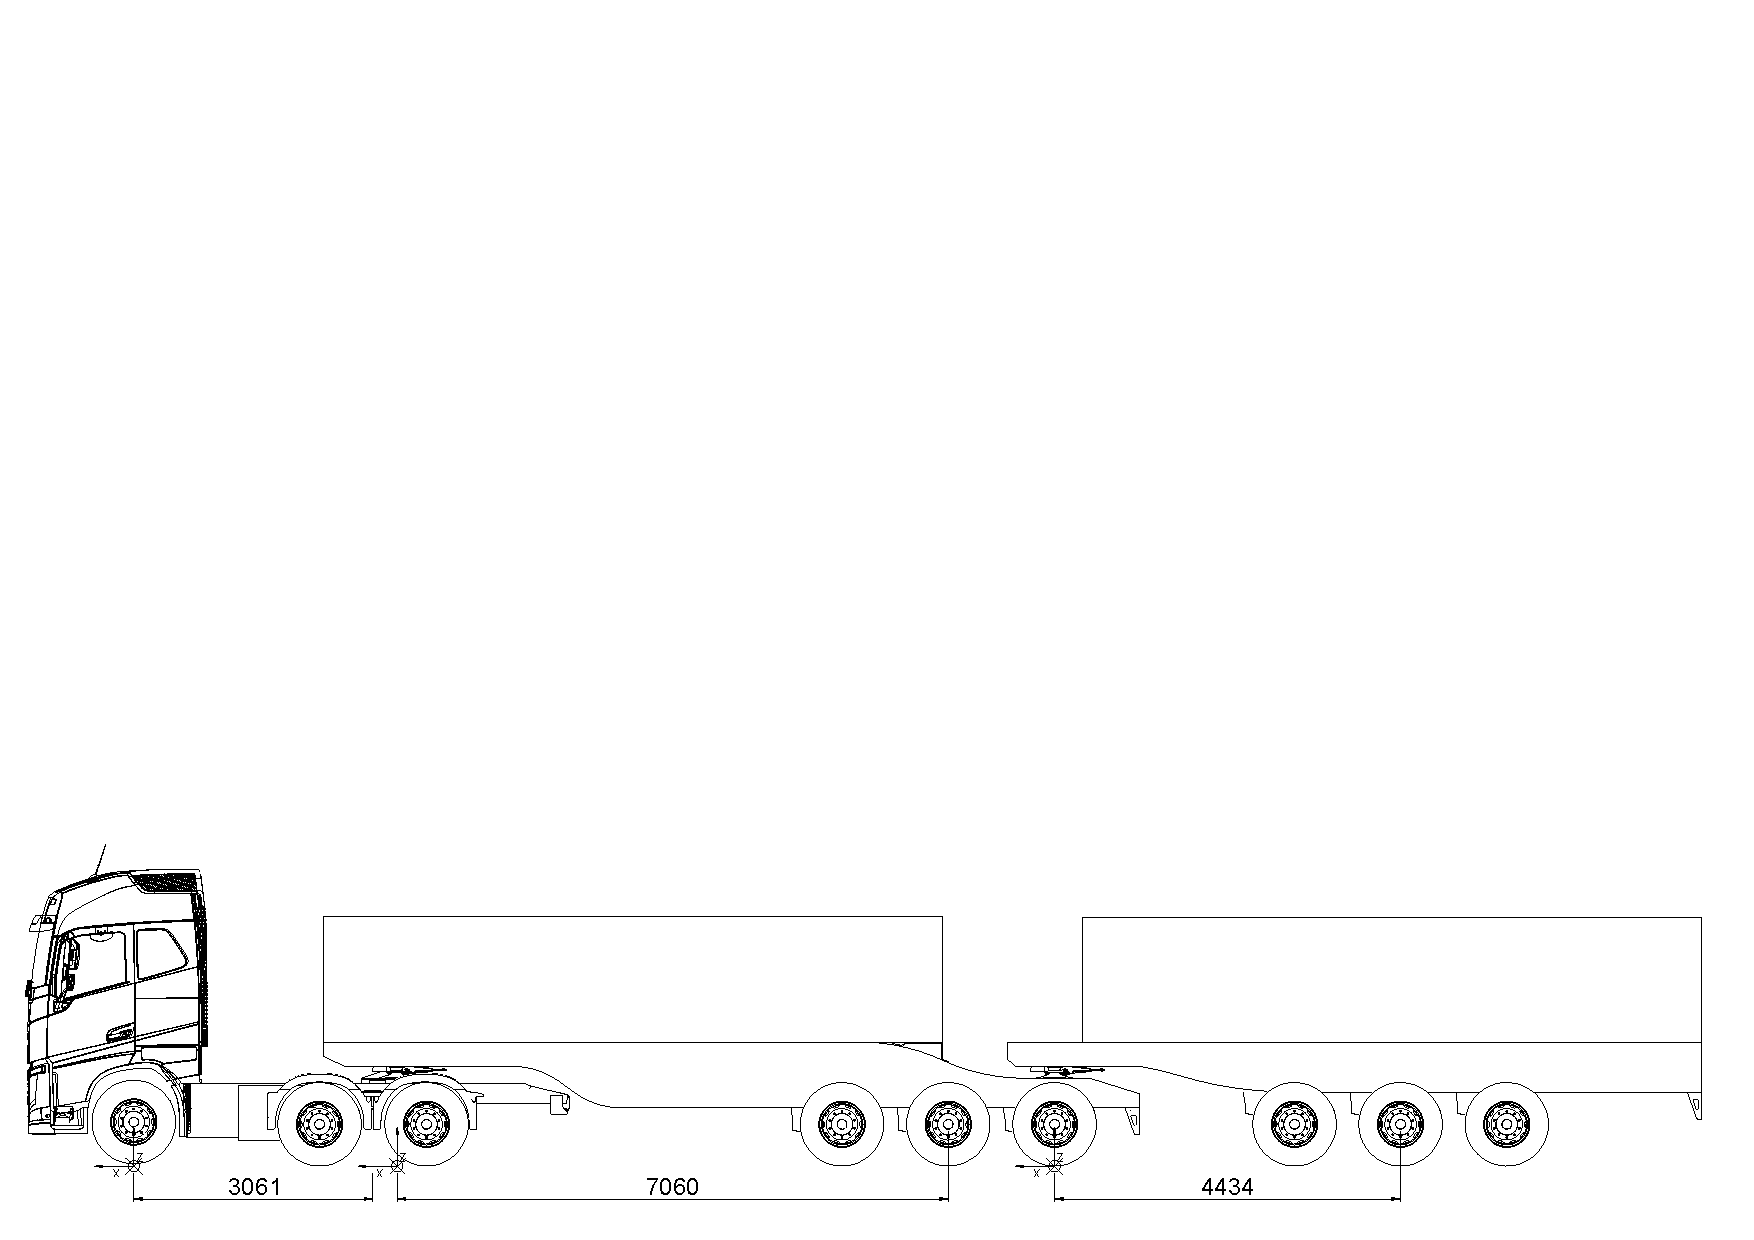
\includegraphics[width=1\textwidth]{fig/parameter-selection_wheelbase_min_b-double}
		\caption{Minimum wheelbase}
	\end{subfigure}%

	\begin{subfigure}[t]{1\textwidth}
		\centering
		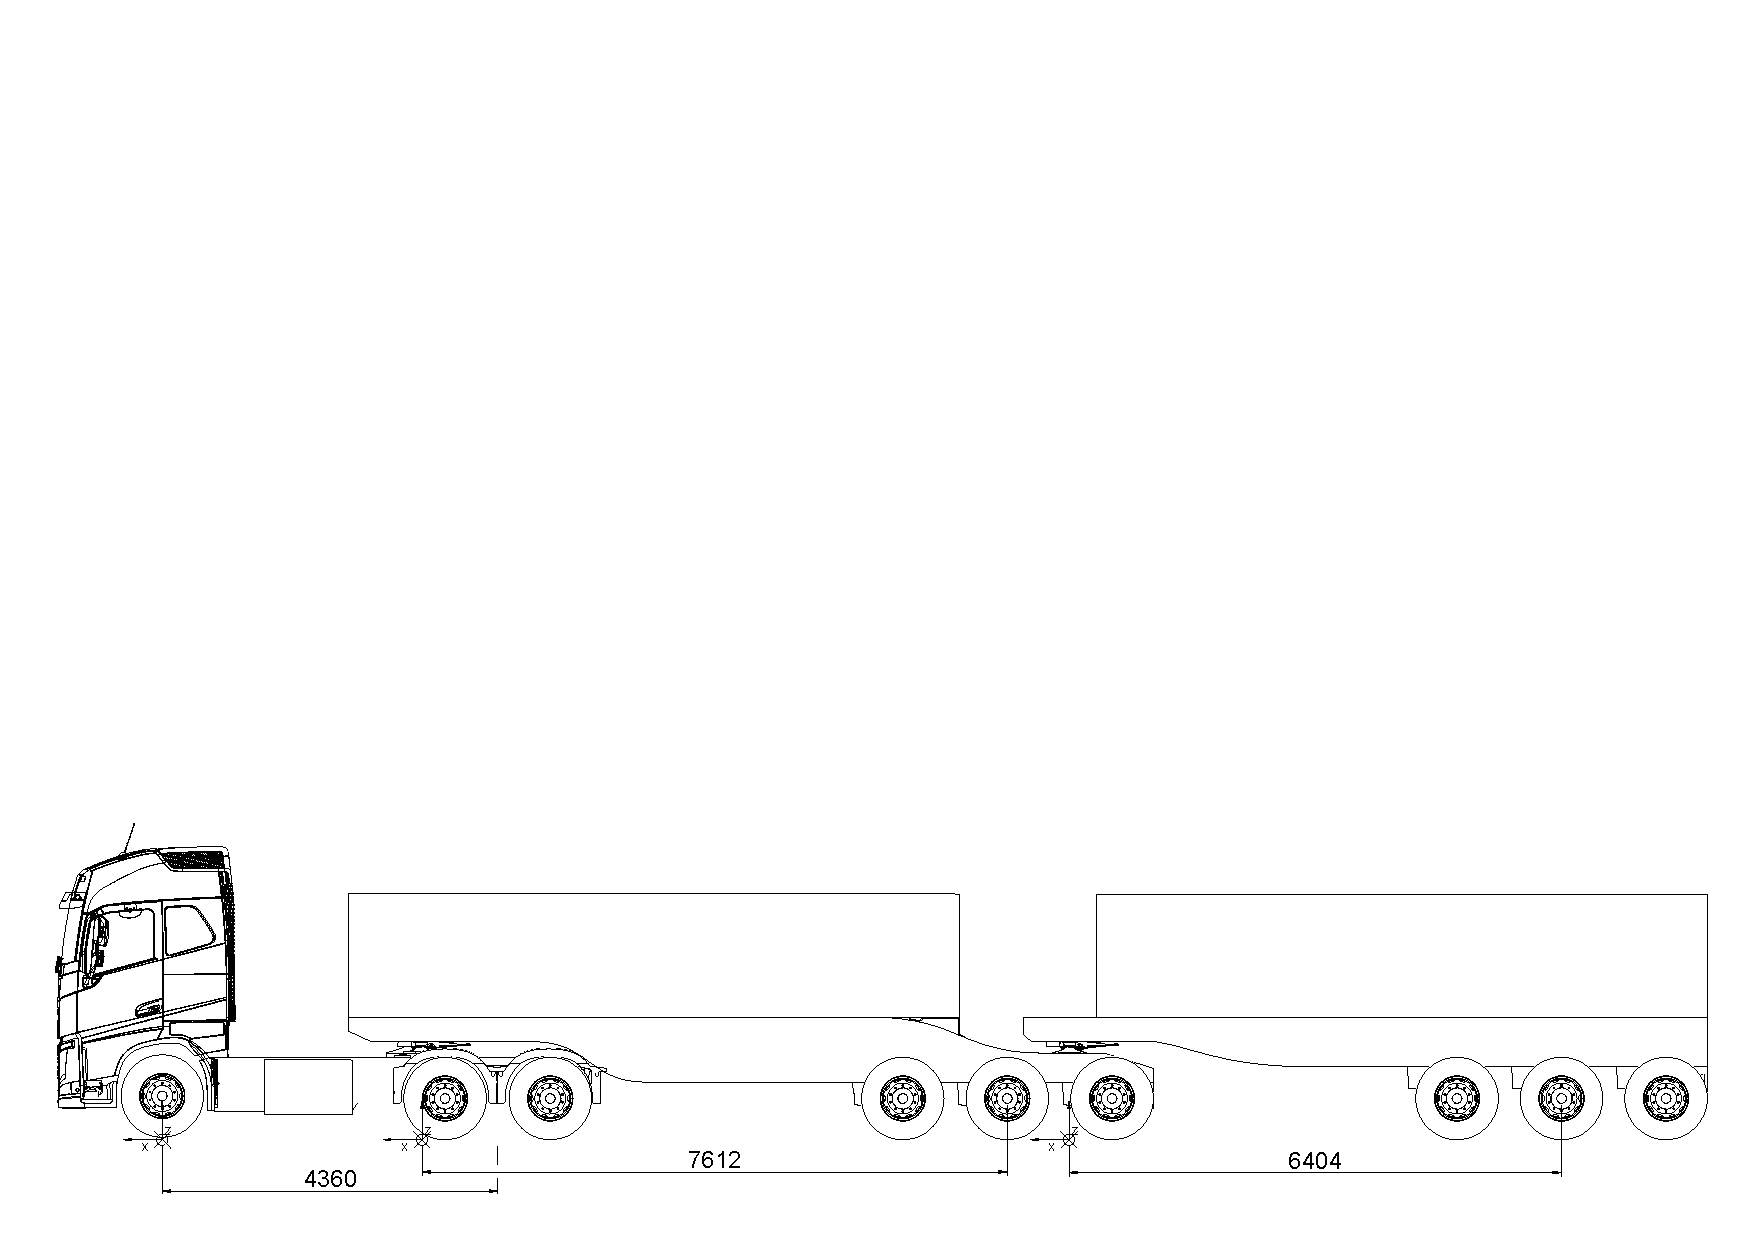
\includegraphics[width=1\textwidth]{fig/parameter-selection_wheelbase_max_b-double}
		\caption{Maximum wheelbase}
	\end{subfigure}

	\caption{Parameter selection - wheelbases for the tridem interlink combination}
	\label{figure:parameter-selection-wheelbase-b-double}
\end{figure*}
%----------------------------------------------
%      FIGURE
%----------------------------------------------

%----------------------------------------------
%      FIGURE
%----------------------------------------------
\begin{figure*}[!htbp]
	\centering
	\begin{subfigure}[t]{1\textwidth}
		\centering
		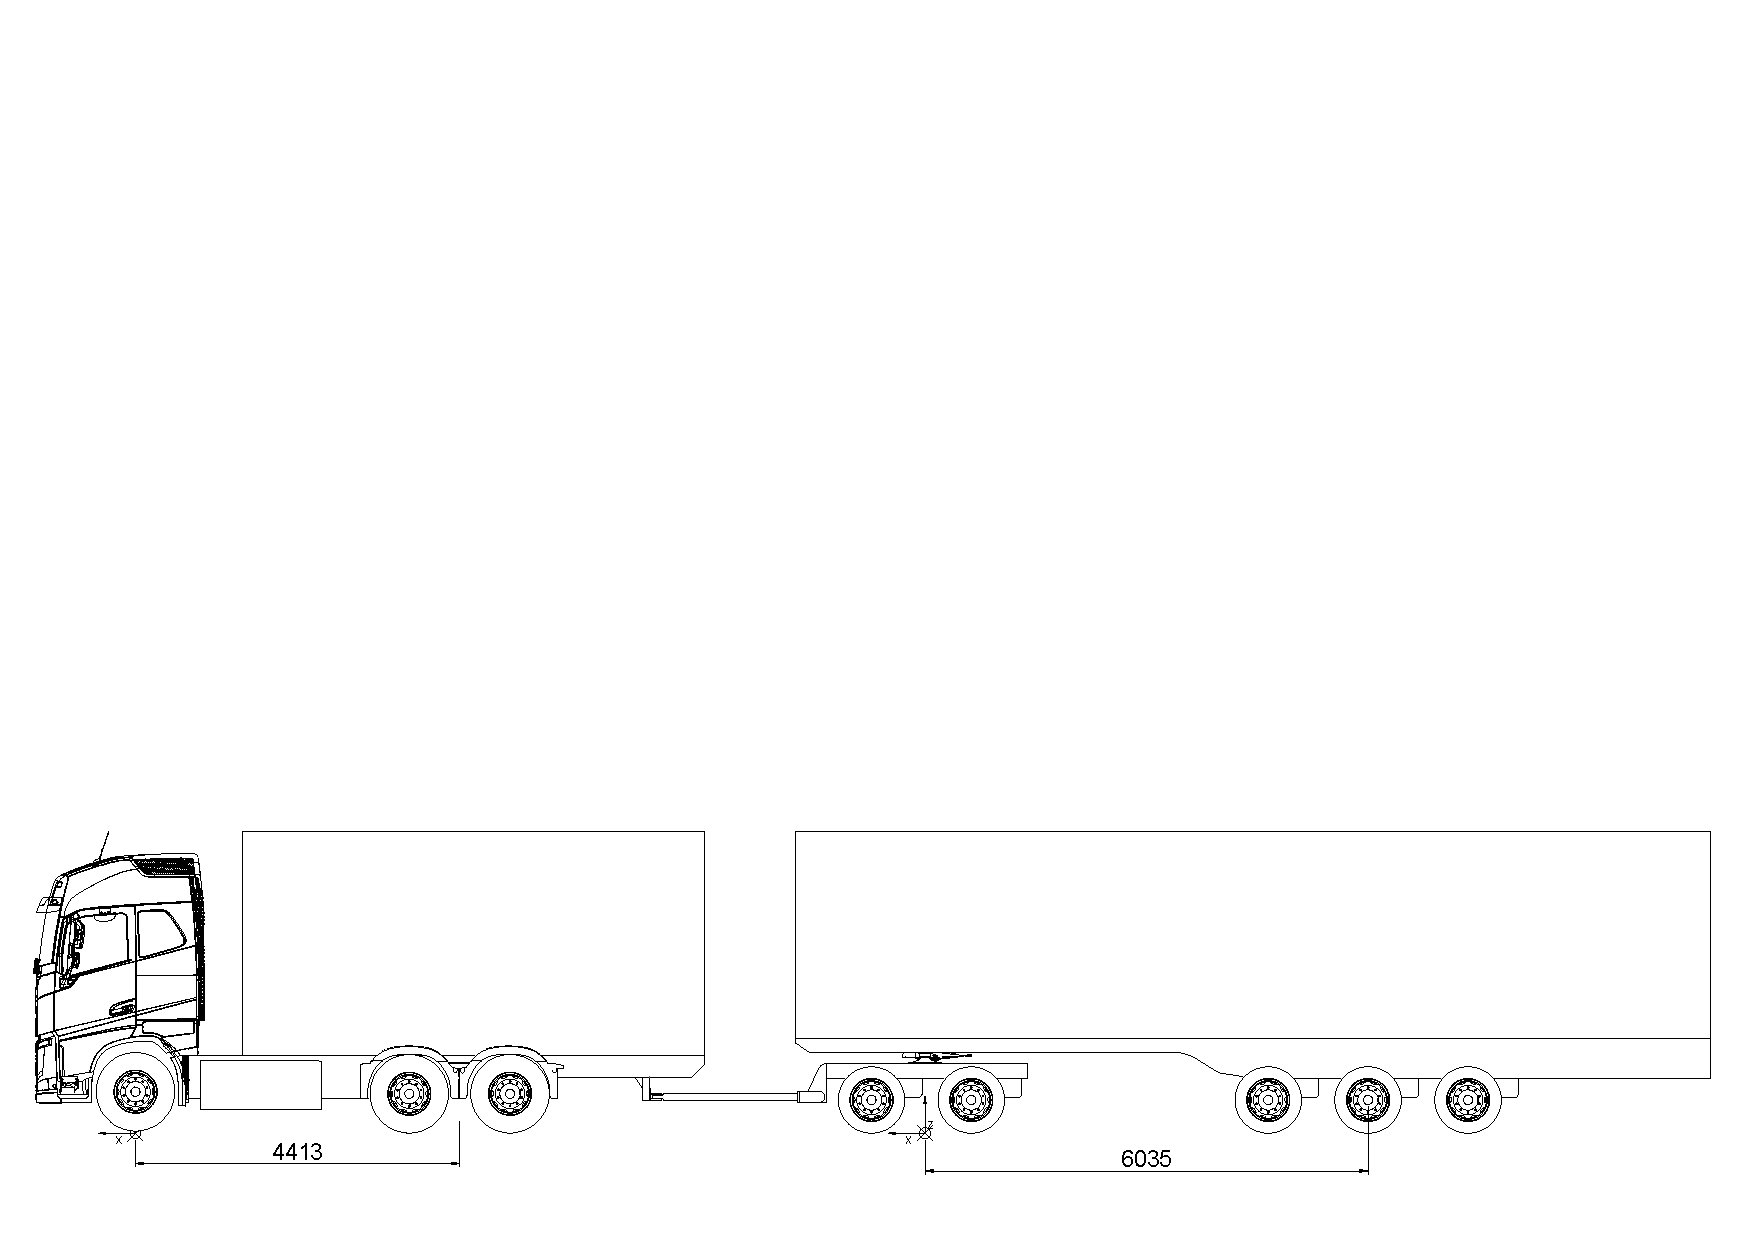
\includegraphics[width=1\textwidth]{fig/parameter-selection_wheelbase_min_truck-and-dog}
		\caption{Minimum wheelbase}
	\end{subfigure}%

	\begin{subfigure}[t]{1\textwidth}
		\centering
		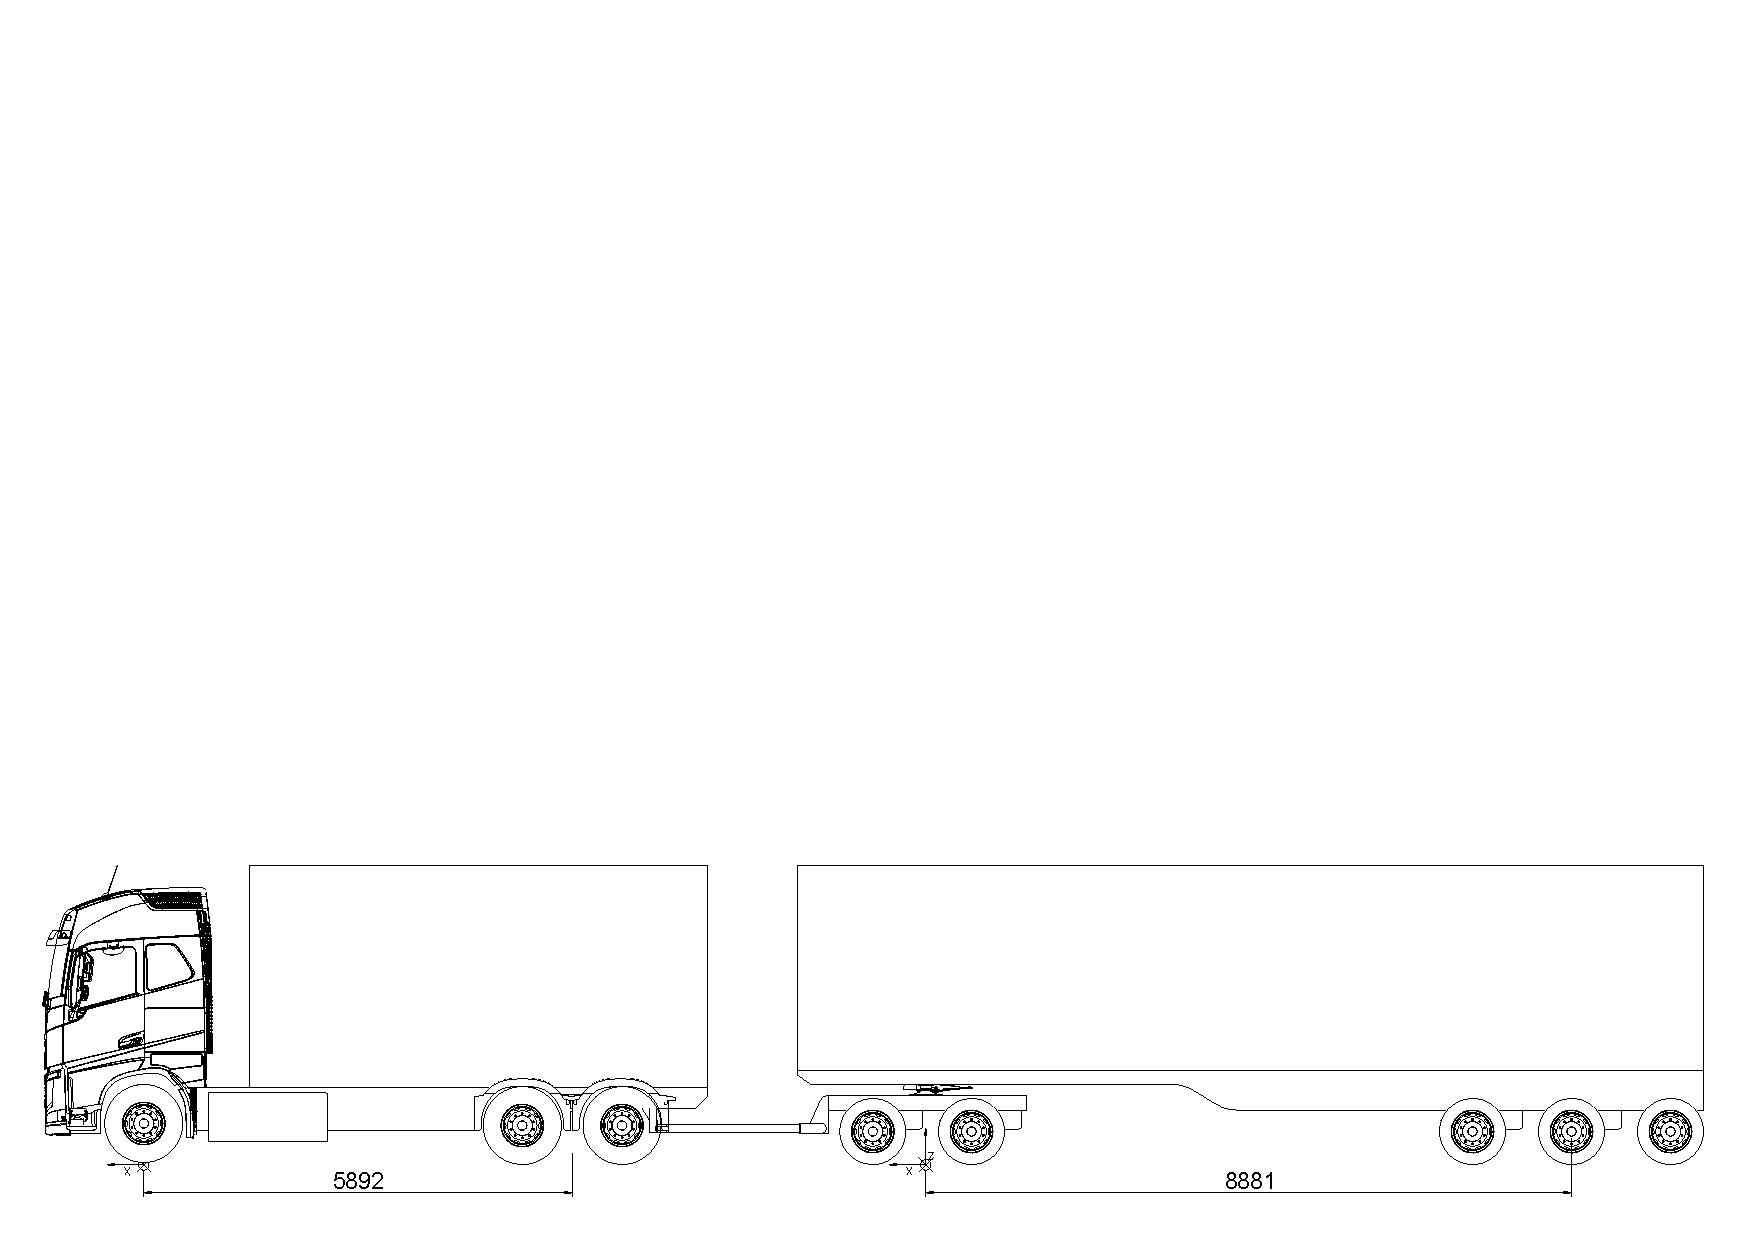
\includegraphics[width=1\textwidth]{fig/parameter-selection_wheelbase_max_truck-and-dog}
		\caption{Maximum wheelbase}
	\end{subfigure}

	\caption{Parameter selection - wheelbases for the rigid drawbar combination}
	\label{figure:parameter-selection-wheelbase-truck-and-dog}
\end{figure*}
%----------------------------------------------
%      FIGURE
%----------------------------------------------

A summary of the range of wheelbases evaluated for each vehicle unit is included in Table~\ref{table:parameter-range-wheelbase}.

%----------------------------------------------
%      TABLE - UPDATED TO NEW RANGES
%----------------------------------------------
\begin{table}[H]
	\centering\footnotesize
	\begin{threeparttable}

		\begin{tabulary}{\textwidth}{lcccll}
			\toprule
			\textbf{Vehicle unit} & \textbf{Baseline (mm)} & \textbf{Min. (mm)} & \textbf{Max. (mm)} & \textbf{Rationale min.} & \textbf{Rationale max.} \\
			\midrule
            Truck tractor & 3885  & 3061  & 4360  & Regulation 226 (2)(c) & Structural \\
            Rigid truck & 5285  & 4413  & 5892  & Regulation 226 (2)(c) & Structural \\
            Quad semi-trailer & 10000 & 7975  & 10000 & Model stability & Regulation 225 (b) \\
            Tridem interlink leader & 7420  & 7060  & 7612  & Hitch location & Structural \\
            Tridem interlink follower & 5950  & 4434  & 6404  & Model stability & Structural \\
            Tridem semi-trailer & 8255  & 6035  & 8881  & Model stability & Structural \\
			\bottomrule
		\end{tabulary}

		\caption{Parameter range - wheelbase}
		\label{table:parameter-range-wheelbase}

		% 		\begin{tablenotes}
		% 			\item[1] %\tnote{1}
		% 		\end{tablenotes}

	\end{threeparttable}
\end{table}
%----------------------------------------------
%      TABLE
%----------------------------------------------

%      SUBSECTION
%----------------------------------------------
\subsection{Dolly Wheelbase (Drawbar Length)}\label{section:drawbar-length}

The range for the dolly wheelbase was determined according to the range of allowed drawbar lengths. Regulation 222 (2b) states the length of an underslung drawbar may exceed 2~m in length if the distance between the two vehicles does not exceed 2.5~m. Using this regulation, the maximum allowed drawbar length is 3451~mm as shown in Figure~\ref{figure:maximum-drawbar-length-according-to-regulation-222-2b}.

%----------------------------------------------
%      FIGURE
%----------------------------------------------
\begin{figure}[H]
	\centering
	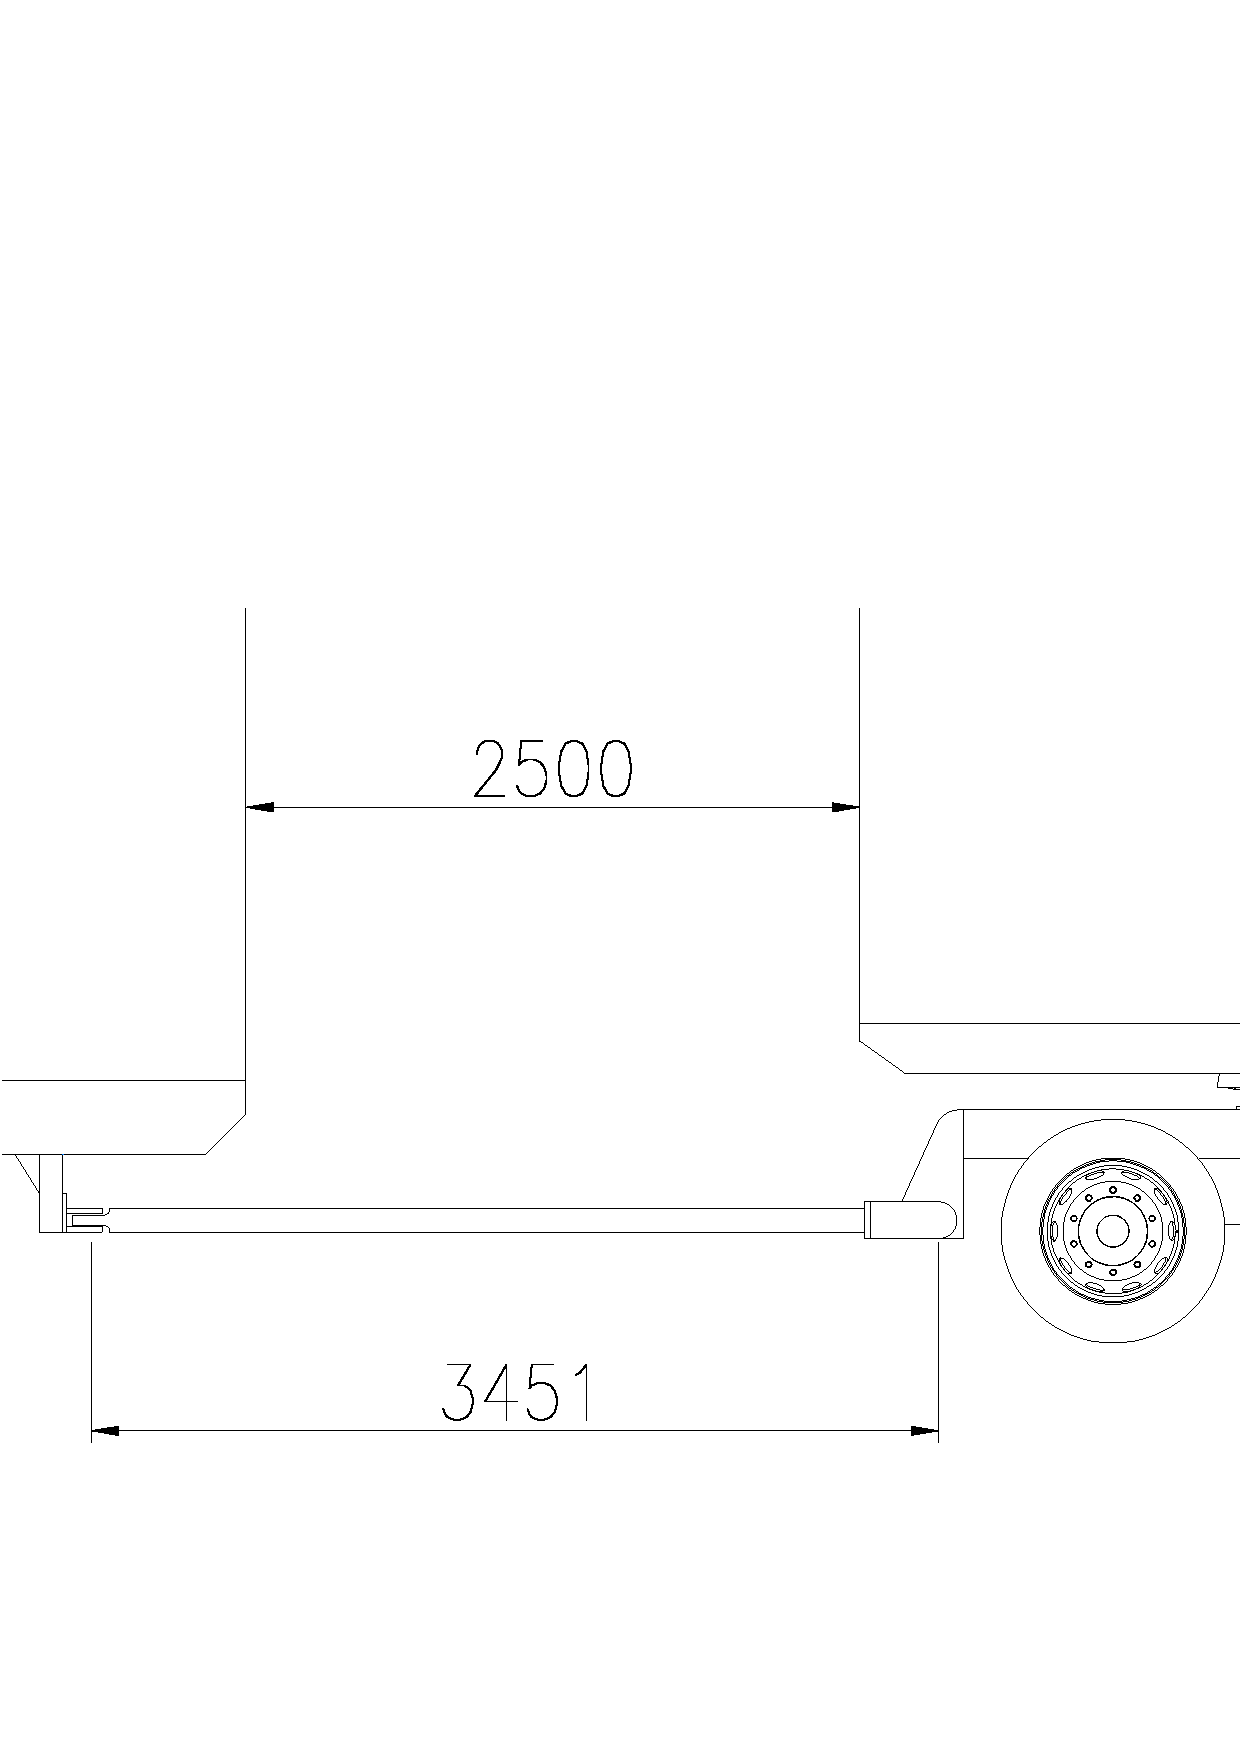
\includegraphics[width=0.5\textwidth]{fig/baseline-pintle-hitch-maximum-length}
	\caption{Maximum drawbar length according to regulation 222 (2b)}
	\label{figure:maximum-drawbar-length-according-to-regulation-222-2b}
\end{figure}
%----------------------------------------------
%      FIGURE
%----------------------------------------------

The minimum drawbar length was chosen such that there would be a 50~mm clearance between the trailer swing radius and the rigid truck chassis resulting in a minimum drawbar length of 1429~mm as shown in Figure~\ref{figure:minimum-drawbar-length}.

%----------------------------------------------
%      FIGURE
%----------------------------------------------
\begin{figure}[H]
	\centering
	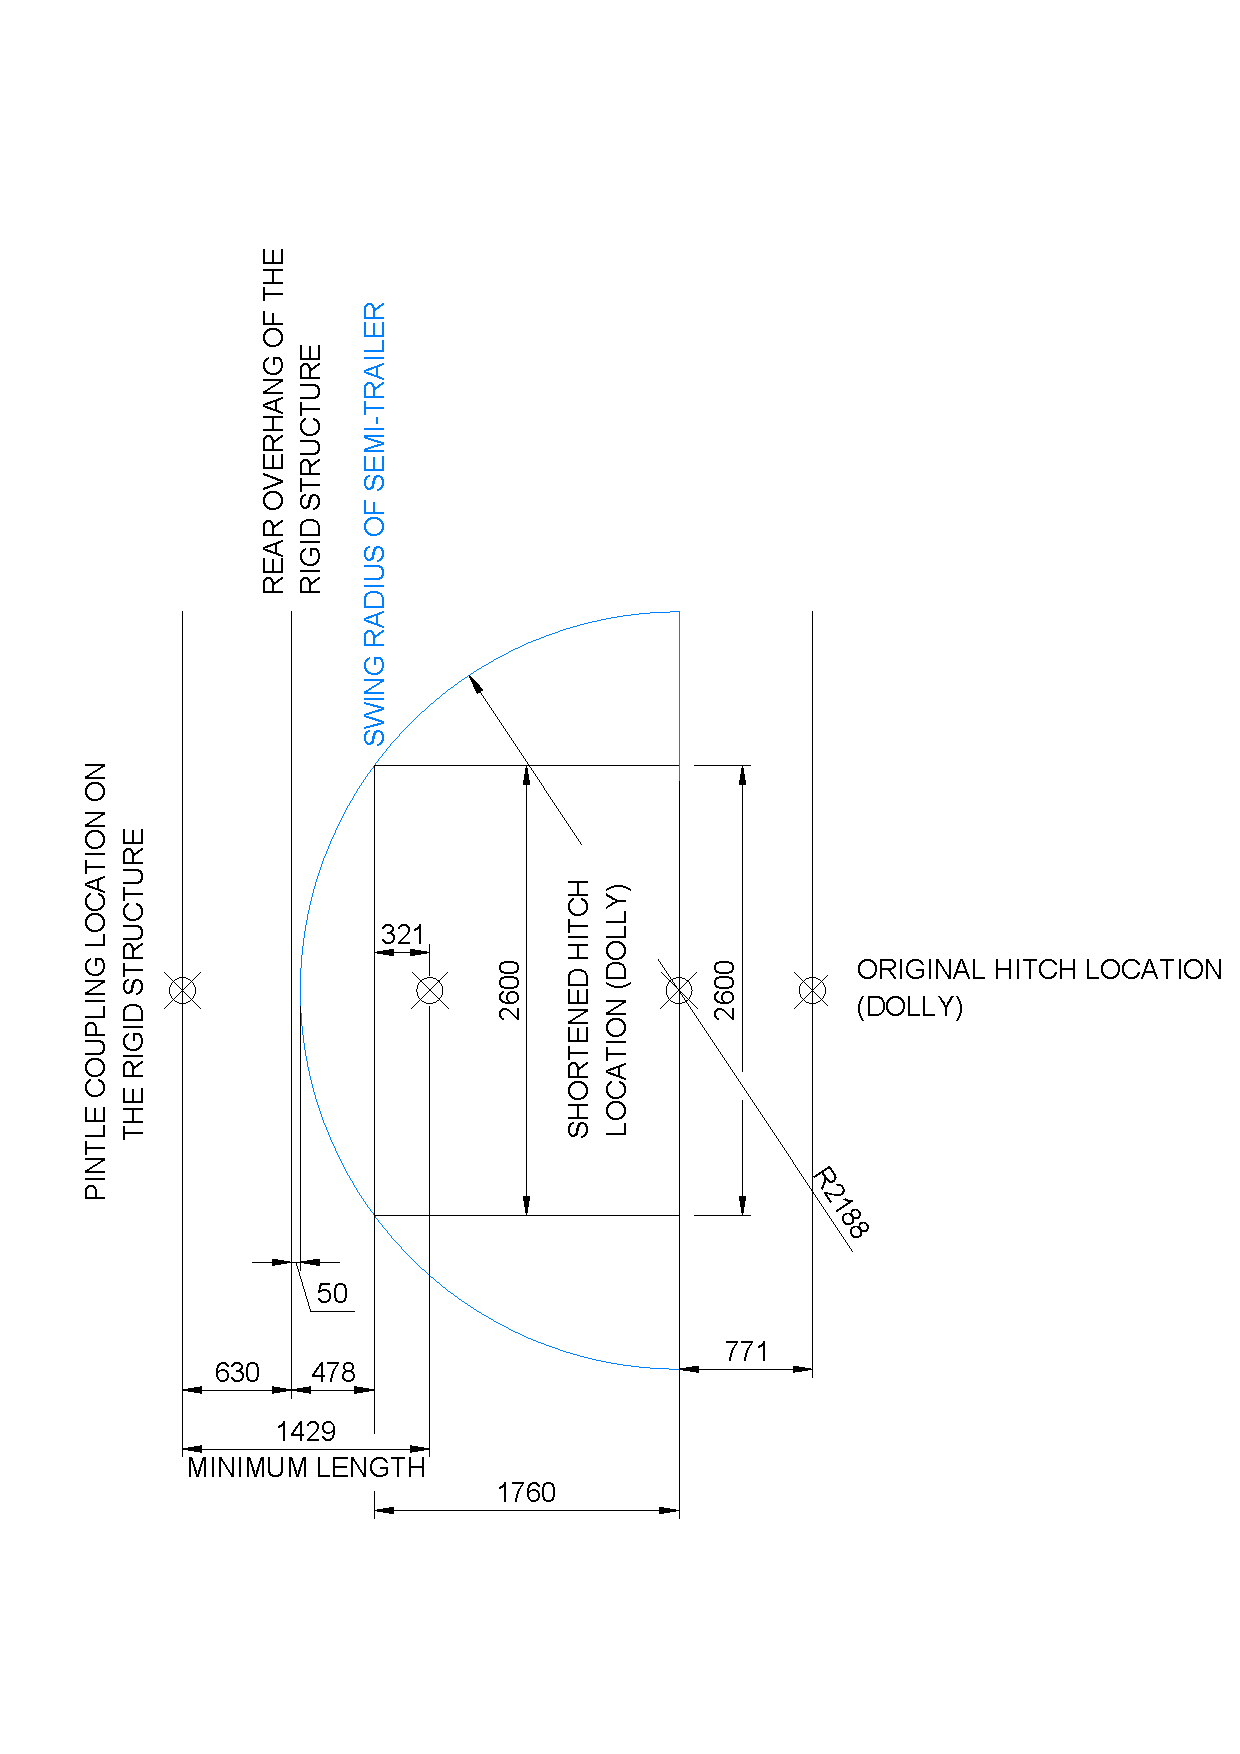
\includegraphics[width=0.7\textwidth]{fig/baseline-pintle-hitch-minimum-length}
	\caption{Minimum drawbar length}
	\label{figure:minimum-drawbar-length}
\end{figure}
%----------------------------------------------
%      FIGURE
%----------------------------------------------

%----------------------------------------------
%      TABLE - UPDATED TO NEW RANGES
%----------------------------------------------
\begin{table}[H]
	\centering\footnotesize
	\begin{threeparttable}

		\begin{tabulary}{\textwidth}{lcccll}
			\toprule
			\textbf{Details} & \textbf{Baseline (mm)} & \textbf{Min. (mm)} & \textbf{Max. (mm)} & \textbf{Rationale Min.} & \textbf{Rationale Max.} \\

			\midrule
			Drawbar length & 2200  & 1429  & 3451  & Structural & Regulation 222 (3) \\
			Wheelbase      & 3590  & 2819  & 4841  & Drawbar length & Drawbar length \\
			\bottomrule

		\end{tabulary}

		\caption{Parameter range - dolly wheelbase and drawbar length}
		\label{table:parameter-range-dolly-pintle-hitch-length}

		%\begin{tablenotes}
		%\item[1] %\tnote{1}
		%\end{tablenotes}

	\end{threeparttable}
\end{table}
%----------------------------------------------
%      TABLE
%----------------------------------------------

%      SUBSECTION
%----------------------------------------------
\subsection{Axle Spacing}\label{section:pr-axle-spacing}

The only publicly available legislation that could be found that explicitly governs axle spacing is the Canadian legislation (British Columbia) \cite{StatutesRegulations} which states that axle spacing should range between 1.2~m to 1.85~m and limits drive axles to a maximum spacing of 1.4~m. This legislation allowed a larger range of variation than typically observed in South Africa (trailer axle spacing of 1360~mm and drive axle spacing of 1400~mm are commonly observed in PBS assessments conducted in South Africa) and was thus deemed to represent a suitable and conservative range of variation for axle spacing.

The drive axle group spacing was varied from 1.2~m to 1.4~m. It was practical to vary all trailer axle group spacing from 1.2~m to 1.85~m as there were no interference's between adjacent axles. The dolly axle group was varied from 1.2~m to 1.8~m since the edge of the front tyre interferes with the pintle hitch position at larger spacing.

The resulting range of axle spacing evaluated for each vehicle unit is summarised in Table~\ref{table:pr-axle-spacing}.

%----------------------------------------------
%      TABLE
%----------------------------------------------
\begin{table}[H]
	\centering\footnotesize
	\begin{threeparttable}

		\begin{tabulary}{\textwidth}{lcccll}
			\toprule
			\textbf{Vehicle unit} & \textbf{Baseline (mm)} & \textbf{Min. (mm)} & \textbf{Max. (mm)} & \textbf{Rationale Min.} & \textbf{Rationale Max.} \\
			\midrule
			Truck tractor & 1370  & 1200  & 1400  & Legislation & Legislation \\
			Rigid truck & 1370  & 1200  & 1400  & Legislation & Legislation \\
			Quad Semi-trailer & 1360  & 1200  & 1850  & Legislation & Legislation \\
			Tridem interlink leader & 1360  & 1200  & 1850  & Legislation & Legislation \\
			Tridem interlink follower & 1360  & 1200  & 1850  & Legislation & Legislation \\
			Tridem semi-trailer & 1360  & 1200  & 1850  & Legislation & Legislation \\
			Dolly & 1360  & 1200  & 1800  & Legislation & Structural limitation \\
			\bottomrule
		\end{tabulary}

		\caption{Parameter range - axle spacing}
		\label{table:pr-axle-spacing}

		%\begin{tablenotes}
		%\item[1] %\tnote{1}
		%\end{tablenotes}

	\end{threeparttable}
\end{table}
%----------------------------------------------
%      TABLE
%----------------------------------------------

%      SUBSECTION
%----------------------------------------------
\subsection{Hitch Longitudinal Location}\label{section:pr-hitch-long-locations}

Common longitudinal hitch positions on tractors were measured by Fancher et al. \cite{Fancher1986}. Hitch positions were measured relative to the centre of the rear axle or rear axle group of between 0" and 24" (610 mm) forward of the rear axle or centre of the tandem axle group.

\textbf{Truck-tractor (5th wheel):}
Longitudinal positions for the tractor hitch position provided by the OEM\footnote{Permission was not received to mention the name of the OEM} correlated well with the data from Fancher et al. with hitch locations from 0~mm to 685~mm forward of the drive axle tandem group. The \gls{oem} range was evaluated for the largest range of possible locations.

\textbf{Rigid truck (pintle hitch):}
It was assumed that the pintle hitch could be mounted on the rigid truck chassis from the edge of the chassis up until the hitch position reached 50~mm from the rearmost drive tyre.

\textbf{Tridem interlink leader (5th wheel):}
The location of the hitch on the tridem interlink leader trailer is largely governed by the limited space on the chassis. It was graphically determined that limits of -380 and +620 from the baseline position would be possible with minimal modifications to the chassis design. The hitch centreline was not allowed further rear than the centreline of the last axle in the axle group. An illustration showing the graphically determined baseline, minimum and maximum position is shown in Figure~\ref{figure:b-double-5th-wheel-hitch-locations}.

%----------------------------------------------
%      FIGURE
%----------------------------------------------
\begin{figure}[H]
	\centering
	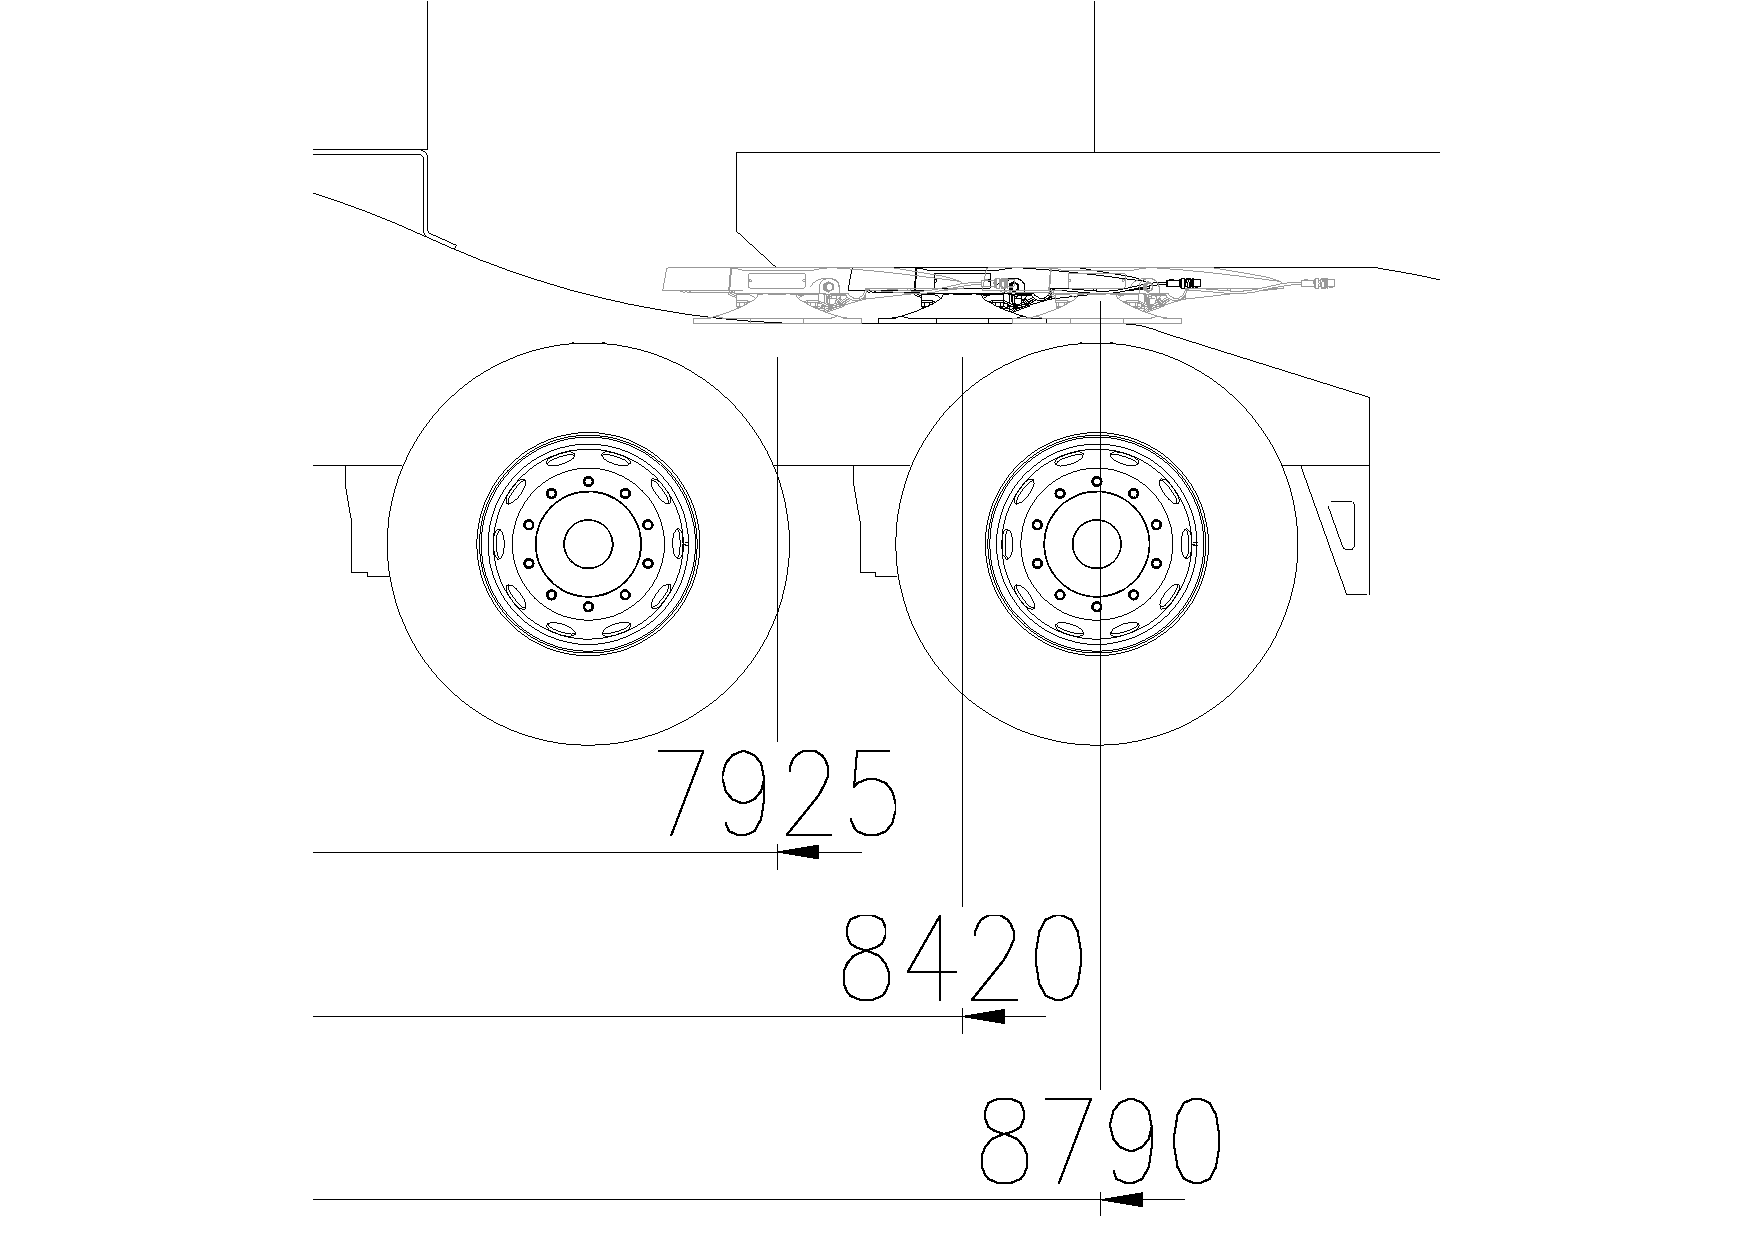
\includegraphics[width=0.5\textwidth]{fig/baseline_b-double_hitch-locations}
	\caption{5th wheel longitudinal locations for the tridem interlink leader trailer}
	\label{figure:b-double-5th-wheel-hitch-locations}
\end{figure}
%----------------------------------------------
%      FIGURE
%----------------------------------------------

\textbf{Rigid drawbar combination dolly (5th wheel):}
The typical 5th wheel location should be located at or near the centre of the dolly to avoid instabilities, it was hence assumed that the dolly 5th wheel location could only be moved +/-200 mm from the centre of the dolly axle group.

A summary of the evaluated hitch locations as discussed above is included in Table~\ref{table:pr-longitudinal-hitch-locations}.

%----------------------------------------------
%      TABLE - UPDATED TO NEW RANGES
%----------------------------------------------
\begin{table}[H]
	\centering\footnotesize
	\begin{threeparttable}

		\begin{tabulary}{\textwidth}{lccc}
			\toprule
			\textbf{Vehicle unit} & \textbf{Baseline (mm)\tnote{1}} & \textbf{Min. (mm)} & \textbf{Max. (mm)} \\
			\midrule
            Truck tractor & -3375 & -3200 & -3885 \\
            Rigid truck & -7115 & -6558 & -7860 \\
            Tridem interlink leader & -8420 & -7925 & -8780 \\
            Dolly & -3639 & -3385 & -3785 \\
			\bottomrule
		\end{tabulary}

		\caption{Parameter range - longitudinal hitch locations}
		\label{table:pr-longitudinal-hitch-locations}

		\begin{tablenotes}
			\item[1] SAE up co-ordinate system and origin taken from centre of steer axle or hitch point at ground level
		\end{tablenotes}

	\end{threeparttable}
\end{table}
%----------------------------------------------
%      TABLE
%----------------------------------------------

%      SUBSECTION
%----------------------------------------------
\subsection{Hitch Height}\label{section-pr-hitch-height}

\textbf{5th wheel:} The 5th wheel hitch heights (truck tractor, tridem interlink leader, and dolly) were assumed to vary from 20~mm above the deck of each vehicle unit (for low-profile 5th wheels), up until a maximum of 1350~mm which is a maximum that has been observed from \gls{pbs} assessments in South Africa.

\textbf{Pintle hitch:} The minimum pintle hitch height for the rigid truck was assumed to be 300 mm above the ground to ensure that the cross chains do not hit the floor. The maximum pintle hitch height was assumed to be at the centre of the rigid truck chassis. While this may not be physically possible in the case of the underslung pintle arrangement, it is possible if the pintle hitch is connected to the rear of the rigid truck chassis. To be inclusive of other pintle hitch arrangements, the full range of possible heights were evaluated.

The resulting range of hitch heights evaluated is summarised in Table~\ref{table:pr-hitch-heights}.

%----------------------------------------------
%      TABLE - UPDATED TO NEW RANGES
%----------------------------------------------
\begin{table}[H]
	\centering\footnotesize
	\begin{threeparttable}

		\begin{tabulary}{\textwidth}{lccc}
			\toprule
			\textbf{Vehicle unit} & \textbf{Baseline (mm)\tnote{1}} & \textbf{Min. (mm)} & \textbf{Max. (mm)} \\
			\midrule
            Truck tractor & 1278  & 1088  & 1350 \\
            Rigid truck & 500   & 300   & 918 \\
            Tridem interlink leader & 1278  & 1148  & 1350 \\
            Dolly & 1100  & 970   & 1350 \\
			\bottomrule
		\end{tabulary}

		\caption{Parameter range - hitch heights}
		\label{table:pr-hitch-heights}

		\begin{tablenotes}
		\item[1] Measured relative to the ground
		\end{tablenotes}

	\end{threeparttable}
\end{table}
%----------------------------------------------
%      TABLE
%----------------------------------------------

%==============================================
%      SECTION
%==============================================
\section{Inertial Parameter Limits - Vehicle Units}

The inertial parameters are mainly influenced by the type of commodity being transported. This governs the payload geometry, orientation and the structure of the trailer which is designed to accommodate the payload.

Limited data was available for trailers and prime movers of similar wheelbase and payloads with the same loading deck space. For most of these inertial limits, assumptions were made based on practical operation, experience from performing \gls{pbs} assessments and data from South African \gls{pbs} assessments. The inertial \gls{vdp} ranges for each of the baseline combinations are detailed in the sections that follow.

%      SUBSECTION
%----------------------------------------------
\subsection{Vehicle Unit Sprung Mass}\label{section:pr-vehicle-unit-sprung-masses}
The baseline vehicles operate at or near the legal axle load limits and as a result, the sprung mass of each vehicle unit was varied from a minimum to the baseline value.

The minimum sprung mass was determined by consolidating data from South African \gls{pbs} assessments (see Appendix~\ref{appendix:anonymised-pbs-data}). The ratio of the sprung mass to the wheelbase was found for each trailer and prime mover as per Equation~\ref{equation:sprung-mass-to-wheelbase-ratio}. The minimum sprung mass to wheelbase ratio was then multiplied with the baseline wheelbase to determine the minimum sprung mass of each vehicle unit as per Equation~\ref{equation:min-sprung-wheelbase}.

It was deemed more appropriate to use the sprung mass to axle spacing ratio (see Equations~\ref{equation:sprung-mass-to-axle-spacing} to \ref{equation:min-sprung-axle-spacing}) to determine the minimum sprung mass for the dolly vehicle unit.

%----------------------------------------------
%      EQUATION
%----------------------------------------------
\begin{align}
		\label{equation:sprung-mass-to-wheelbase-ratio}
		&\gls{rsw} = \frac{\gls{msprung}}{\gls{dwb}}\\
		\label{equation:min-sprung-wheelbase}
		&m_{sprung,min} = \gls{rsw} \times d_{wb-baseline}\\
		\label{equation:sprung-mass-to-axle-spacing}
		&\gls{rsa} = \frac{\gls{msprung}}{\gls{daxle}}\\
		\label{equation:min-sprung-axle-spacing}
		&m_{sprung,min} = \gls{rsa} \times d_{axle-baseline}
\end{align}

Where:

\gls{rsw} = Ratio of vehicle unit sprung mass to wheelbase (kg/m)

\gls{rsa} = Ratio of vehicle unit sprung mass to axle spacing (kg/m)

\gls{dwb} = Wheelbase (m)

\gls{daxle} = Axle spacing (m)

\gls{msprung} = Sprung mass (kg)
%----------------------------------------------
%      EQUATION
%----------------------------------------------

The minimum sprung masses were calculated according to Equations~\ref{equation:min-sprung-wheelbase}~to~\ref{equation:min-sprung-axle-spacing} for each vehicle unit and are included in Table~\ref{table:minimum-vehicle-unit-sprung-masses}.

%----------------------------------------------
%      TABLE - UPDATED TO NEW RANGES
%----------------------------------------------
\begin{table}[H]
	\centering\footnotesize
	\begin{threeparttable}

		\begin{tabulary}{\textwidth}{lCCCC}
			\toprule
			\textbf{Vehicle unit} & \textbf{Wheelbase (mm)\tnote{1}} & \textbf{Baseline sprung mass (kg)} & \boldmath{}\textbf{Min. $R_{sw}$ or $R_{sa}$ (kg/m)}\unboldmath{} & \textbf{Min. sprung mass (kg)} \\
			\midrule
             Truck tractor & 3885 & 6598  & 1140  & 4428 \\
             Rigid truck & 5285 & 6698  & 902   & 4767 \\
             Quad semi-trailer & 10000 & 10410 & 250   & 2500 \\
             Tridem interlink leader & 7420 & 4632  & 250   & 1855 \\
             Tridem interlink follower & 5950 & 4167  & 250   & 1488 \\
             Tridem semi-trailer & 8255 & 3150  & 250   & 2064 \\
             Dolly & 1360 & 453   & 294   & 400 \\
			\bottomrule
		\end{tabulary}

		\caption{Minimum sprung mass for each vehicle unit}
		\label{table:minimum-vehicle-unit-sprung-masses}

		\begin{tablenotes}
			\item[1] Or axle spacing in the case of the dolly
		\end{tablenotes}

	\end{threeparttable}
\end{table}
%----------------------------------------------
%      TABLE
%----------------------------------------------

%      SUBSECTION
%----------------------------------------------
\subsection{Vehicle Unit Longitudinal Centre of Gravity}\label{section:pr-cgx-vehicle-units}

The \glsfirst{cgx} for the prime mover is influenced mainly by the cab and chassis design as well as any optional extras. It was assumed that the \gls{cgx} could vary by +/-20\% for both prime movers.

Trailers can differ significantly in design depending on the payload it is intended to haul. However for a specific wheelbase, the \gls{cgx} would not be able to vary by extreme amounts. The variation for the trailer \gls{cgx} was assumed to vary slightly more than for the prime mover at +/-30\% from the baseline value.

The structure of a dolly is relatively compact and has little scope to vary between manufacturers. Thus, a smaller range of variation of +/-10\% from the baseline \gls{cgx} value was assumed.

The resulting range of \gls{cgx} locations for the prime movers is included in Table~\ref{table:parameter-range-cgx-prime-movers} with the locations for the trailers and dolly following in Table~\ref{table:parameter-range-cgx-trailer}.

%----------------------------------------------
%      TABLE
%----------------------------------------------
\begin{table}[H]
	\centering\footnotesize
	\begin{threeparttable}

		\begin{tabulary}{\textwidth}{lccc}
			\toprule
			\textbf{Vehicle unit} & \textbf{Baseline (mm)\tnote{1}} & \textbf{Min. (mm)} & \textbf{Max. (mm)} \\
			\midrule
             Truck tractor & -1001 & -801  & -1201 \\
             Rigid truck & -1860 & -1488 & -2232 \\
			\bottomrule
		\end{tabulary}

		\caption{Parameter range - prime mover \gls{cgx}}
		\label{table:parameter-range-cgx-prime-movers}

		\begin{tablenotes}
			\item[1] SAE up co-ordinate system and origin taken from centre of steer axle or hitch point at ground level
		\end{tablenotes}

	\end{threeparttable}
\end{table}
%----------------------------------------------
%      TABLE
%----------------------------------------------

%----------------------------------------------
%      TABLE
%----------------------------------------------
\begin{table}[H]
	\centering\footnotesize
	\begin{threeparttable}

		\begin{tabulary}{\textwidth}{lccc}
			\toprule
			\textbf{Vehicle unit} & \textbf{Baseline (mm)\tnote{1}} & \textbf{Min. (mm)} & \textbf{Max. (mm)} \\
			\midrule
             Quad semi-trailer & -6455 & -4519 & -8392 \\
             Tridem interlink leader & -3656 & -2559 & -4753 \\
             Tridem interlink follower & -4269 & -2988 & -5550 \\
             Tridem semi-trailer & -5575 & -3903 & -7248 \\
             Dolly & -3450 & -3105 & -3795 \\
			\bottomrule
		\end{tabulary}

		\caption{Parameter range - trailer \gls{cgx}}
		\label{table:parameter-range-cgx-trailer}

		\begin{tablenotes}
			\item[1] SAE up co-ordinate system and origin taken from centre of steer axle or hitch point at ground level
		\end{tablenotes}

	\end{threeparttable}
\end{table}
%----------------------------------------------
%      TABLE
%----------------------------------------------

%      SUBSECTION
%----------------------------------------------
\subsection{Vehicle Unit Lateral Centre of Gravity}\label{section:pr-cgy-vehicle-units}

To account for eccentric loading about the longitudinal axis which could arise due to fuel tanks, spare tools, pneumatic equipment, storage compartments etc., a variation of 10\% of the unit overall width was assumed for both the sprung mass and payload \gls{cgy}.

In the case of the dolly, there would be no reason for lateral eccentricity of the \gls{cgy} and therefore it was not varied.

The range of \gls{cgy} locations evaluated (measured according to the SAE up coordinate system with the origin at the centre of the combination) are:

\begin{itemize}
	\item \textbf{Truck tractor:} +/- 250~mm
	\item \textbf{All other units (excluding the dolly unit):} +/- 260~mm
\end{itemize}

\subsection{Vehicle Unit Vertical Centre of Gravity}\label{section:pr-cgz-vehicle-units}
The \glsfirst{cgz} of a vehicle unit can vary due to various cab and trailer designs for the same wheelbase. A flatbed or stepdeck may have a low sprung mass centre of gravity, while a side tipper or tanker would have a higher sprung mass centre of gravity. To develop a representative range of possible vehicle configurations, the \gls{cgz} locations of various trailers were identified from South African \gls{pbs} assessments and anonymised for presentation in Tables~\ref{table:anonymised-trailer-centre-of-gravities-and-normalised-sprung-masses}~to~\ref{table:anonymised-prime-mover-cgz-and-normalised-sprung-masses} in Appendix~\ref{appendix:anonymised-pbs-data}. The resulting range of \gls{cgz} positions is summarised in Table~\ref{table:parameter-range-cgz}.

%----------------------------------------------
%      TABLE
%----------------------------------------------
\begin{table}[H]
	\centering\footnotesize
	\begin{threeparttable}

		\begin{tabulary}{\textwidth}{lccc}
			\toprule
			\textbf{Vehicle unit} & \textbf{Baseline (mm)\tnote{1}} & \textbf{Minimum (mm)}& \textbf{Maximum (mm)} \\
			\midrule
             Truck tractor & 1204  & 1070  & 1426 \\
             Rigid truck & 1017  & 1000  & 1315 \\
             Quad semi-trailer & 2025  & 1280  & 2025 \\
             Tridem interlink leader & 1777  & 1280  & 2025 \\
             Tridem interlink follower & 1912  & 1280  & 2025 \\
             Tridem semi-trailer & 1500  & 1280  & 2025 \\
			 Dolly & 868 & 868 & 1050 \\
			\bottomrule
		\end{tabulary}

		\caption{Parameter range - vehicle unit \gls{cgz}}
		\label{table:parameter-range-cgz}

		\begin{tablenotes}
			\item[1] SAE up co-ordinate system and origin taken from centre of steer axle or hitch point at ground level
		\end{tablenotes}

	\end{threeparttable}
\end{table}
%----------------------------------------------
%      TABLE
%----------------------------------------------

%      SUBSECTION
%----------------------------------------------
\subsection{Vehicle Unit Roll Moment of Inertia}\label{section:pr-roll-moment-of-inertia-vehicle-units}

The vehicle unit \glsfirst{ixx} is rarely supplied for the purposes of a \gls{pbs} assessment. Most of the engineering drawings provided are drawn in 2D \gls{cad} and 3D models which allow for accurate calculation of the inertial properties are often not available.

Winkler et al. \cite{Winkler2011} and Fancher et al. \cite{Fancher1986} provide simplified estimates for the moment of inertia for conventional trailers and prime movers. These simplified estimates are useful for when measured values are not provided, however they in no way encompass the full range of prime movers. It is presently unsure as to whether using these estimates predicts vehicle performance from simulations conservatively. Since the moment of inertia for a vehicle is not often supplied, to be inclusive of all vehicle designs, broad ranges are developed as discussed in Sections~\ref{section:pr-roll-moment-of-inertia-vehicle-units}~to~\ref{section:pr-pitch-yaw-radius-of-gyration-vehicle-units}.

The radius of gyration (\gls{r}) of an inertial object can be related to the \gls{i} with its mass according to Equation~\ref{equation:radius-of-gyration-from-moment-of-inertia}. The radius of gyration is an easier metric to read and compare and will be used in place of the moment of inertia where possible.

\begin{align}
	\label{equation:radius-of-gyration-from-moment-of-inertia}
	r = \sqrt{\frac{I}{m}}
\end{align}

Where:

$r$ = Radius of gyration (m)

$I$ = Moment of inertia (kg.m\textsuperscript{2})

$m$ = Mass of the inertial object (kg)

%      SUBSUBSECTION
%----------------------------------------------
\subsubsection{Prime mover units}\label{section:pr-roll-moment-of-inertia-prime-mover-vehicle-units}

Fancher et al. \cite{Fancher1986} measured the \glsfirst{rx} of the sprung mass for some prime movers. The roll radius of gyration for each of the measured vehicles was calculated using Equation~\ref{equation:radius-of-gyration-from-moment-of-inertia} and the results are displayed in Table~\ref{table:measured-values-for-prime-mover-rx-from-fancher-et-al}.

Comparing calculated \gls{rx} values to that of the baseline prime movers (see Table~\ref{table:variation-of-estimated-rx-measurements-from-Fancher-et-al-prime-mover}), a minimum variation of 75\% and a maximum variation of 95\% was observed. Due to the small sample of measured values and considering that the measured data encompasses only USA native cab styles, a conservative variation of +/-30\% was chosen to encapsulate all varieties of prime movers and cab designs, therefore:

\begin{itemize}
\item \textbf{Prime mover \gls{rx} variation:} +/-30\%
\end{itemize}

%----------------------------------------------
%      TABLE
%----------------------------------------------
\begin{table}[H]
	\centering\footnotesize
	\begin{threeparttable}

		\begin{tabulary}{\textwidth}{lCCCC}
			\toprule
			\textbf{Vehicle description} & \textbf{Tare mass (kg)} & \textbf{Estimated sprung mass (kg)} & \textbf{\gls{ixx} (kg.m\sstw)} & \textbf{\gls{rx} (m)} \\
			\midrule
			Ford 9000 (WB = 185.75") & 7772  & 5051  & 2869  & 0.608 \\
			GMC Astro 95 Tractor (WB = 150") & 7888  & 5166  & 2582  & 0.572 \\
			GMC Tractor & 4933   & 3300  & 2576  & 0.723 \\
			Ford 800 Conventional Tractor (WB = 150") & 5163     & 2442  & 2576  & 0.706 \\
			International Harvester Tractor (WB = 143") & 6695    & 3974  & 2518  & 0.613 \\
			\bottomrule
		\end{tabulary}

		\caption{Measured values for prime mover \gls{rx} estimated from Fancher et al. \cite{Fancher1986}}
		\label{table:measured-values-for-prime-mover-rx-from-fancher-et-al}

		%\begin{tablenotes}
		%\item[1] %\tnote{1}
		%\end{tablenotes}

	\end{threeparttable}
\end{table}
%----------------------------------------------
%      TABLE
%----------------------------------------------

%----------------------------------------------
%      TABLE
%----------------------------------------------
\begin{table}[H]
	\centering\footnotesize
	\begin{threeparttable}

		\begin{tabulary}{\textwidth}{lccc}
			\toprule
			\textbf{Baseline description} & \textbf{Baseline \gls{rx} (m)} & \textbf{Min. variation (\%)} & \textbf{Max. variation (\%)} \\
			\midrule
			All prime movers & 0.76 & 75\%  & 95\% \\
			\bottomrule
		\end{tabulary}

		\caption{Variation of estimated prime mover \gls{rx} measurements from Fancher et al. \cite{Fancher1986}}
		\label{table:variation-of-estimated-rx-measurements-from-Fancher-et-al-prime-mover}

		%\begin{tablenotes}
		%\item[1] %\tnote{1}
		%\end{tablenotes}

	\end{threeparttable}
\end{table}
%----------------------------------------------
%      TABLE
%----------------------------------------------

%      SUBSUBSECTION
%----------------------------------------------
\subsubsection{Trailer and dolly units}\label{section:pr-roll-moment-of-inertia-trailer-vehicle-units}

A similar exercise was performed with measured data for trailers from Fancher et al. \cite{Fancher1986}. The calculated \gls{rx} for the measured trailers is provided in Table~\ref{table:measured-values-for-trailer-rx-from-fancher-et-al}.

%----------------------------------------------
%      TABLE
%----------------------------------------------
\begin{table}[H]
	\centering\footnotesize
	\begin{threeparttable}

		\begin{tabulary}{\textwidth}{lCCCC}
			\toprule
			\textbf{Typical tare masses} & \textbf{Tare mass (kg)} & \textbf{Estimated sprung mass (kg)} & \textbf{\gls{ixx} (kg.m\sstw)} & \textbf{\gls{rx} (m)} \\
			\midrule
			48" Semi-trailer, tandem axle (WB=40') & 6260    & 4663  & 9039  & 1.202 \\
			45' Semi-trailer, tandem axle (WB=37') & 5916    & 4320  & 8405  & 1.192 \\
			42' Semi-trailer, tandem axle (WB=36') & 5573     & 3976  & 7769  & 1.181 \\
			28' Semi-trailer, single axle (WB=21') & 2981    & 2183  & 5934  & 1.411 \\
			27' Semi-trailer, single axle, (WB=21') & 2948    & 2150  & 5649  & 1.384 \\
			\bottomrule
		\end{tabulary}

		\caption{Measured values for trailer \gls{rx} calculated from Fancher et al. \cite{Fancher1986}}
		\label{table:measured-values-for-trailer-rx-from-fancher-et-al}

		%\begin{tablenotes}
		%\item[1] %\tnote{1}
		%\end{tablenotes}

	\end{threeparttable}
\end{table}
%----------------------------------------------
%      TABLE
%----------------------------------------------

In comparison to the baseline trailer \gls{rx} (see Table~\ref{table:variation-of-estimated-rx-measurements-from-Fancher-et-al-trailer}), the measured values varied by from 43\% higher to 36\% lower. Using this as a guideline and acknowledging that the measured data represents only a small sample of trailer designs, a conservative range of +/-45\% was evaluated. No data was available for dollies. Due to their design being inherently simpler, it was assumed to vary by +/-20\% and therefore:


\begin{itemize}
\item \textbf{Trailer \gls{rx} variation:} +/-45\%
\item \textbf{Dolly \gls{rx} variation:} +/-20\%
\end{itemize}

%----------------------------------------------
%      TABLE
%----------------------------------------------
\begin{table}[H]
	\centering\footnotesize
	\begin{threeparttable}

		\begin{tabulary}{\textwidth}{lccc}
			\toprule
			\textbf{Baseline description} & \textbf{Baseline \gls{rx} (m)} & \textbf{Min. variation (\%)} & \textbf{Max. variation (\%)} \\
			\midrule
			Quad semi-trailer & 1.588 & 74\%  & 89\% \\
			Tridem interlink leader & 0.985 & 120\% & 143\% \\
			Tridem interlink follower & 1.007 & 117\% & 140\% \\
			Tridem semi-trailer & 1.277 & 92\%  & 110\% \\
			\bottomrule
		\end{tabulary}

		\caption{Variation of estimated trailer \gls{rx} measurements from Fancher et al. \cite{Fancher1986}}
		\label{table:variation-of-estimated-rx-measurements-from-Fancher-et-al-trailer}

		%\begin{tablenotes}
		%\item[1] %\tnote{1}
		%\end{tablenotes}

	\end{threeparttable}
\end{table}
%----------------------------------------------
%      TABLE
%----------------------------------------------

%      SUBSECTION
%----------------------------------------------
\subsection{Vehicle Unit Pitch and Yaw Moment of Inertia}\label{section:pr-pitch-yaw-radius-of-gyration-vehicle-units}

The \gls{iyy} and \glsfirst{izz} are approximately equal for a vehicle unit and were treated as a single \gls{vdp}.

The sprung mass can be distributed with more variability along the pitch and yaw axes, especially in the case of superstructures designed to accommodate specialised loads. Thus, the \gls{ry} and \glsfirst{rz} were assumed to vary by +/-40\% for the prime mover units and +/-50\% for the trailer units with the intent to encompass the wide variety of trailer, prime mover and cab designs. No data was available for dollies and due to their inherently simpler design, it was assumed to vary by +/-30\% and therefore:

\begin{itemize}
\item \textbf{Prime mover \gls{ry} / \gls{rz} variation:} +/- 40\%
\item \textbf{Trailer \gls{ry} / \gls{rz} variation:} +/-50\%
\item \textbf{Dolly \gls{ry} / \gls{rz} variation:} +/-30\%
\end{itemize}


%==============================================
%      SECTION
%==============================================
\section{Inertial Parameter Limits - Payloads}\label{section:pr-inertial-parameter-limits-payloads}

The inertial properties of the payload are dependent on the type of commodity being transported as well as the available loading deck area. The sections that follow discuss the ranges determined for the inertial properties of the payloads.

%      SUBSECTION
%----------------------------------------------
\subsection{Payload Mass}\label{section:pr-payload-masses}

The baseline combinations operate at or near the legal axle load limits. As a result the payload masses were assumed to vary from 0~kg for operation in the unladen state up to the baseline payload mass. The payloads for each unit are included in Table~\ref{table:parameter-range-payload-masses}.

%----------------------------------------------
%      TABLE - UPDATED TO NEW RANGES
%----------------------------------------------
\begin{table}[H]
	\centering\footnotesize
	\begin{threeparttable}

		\begin{tabulary}{\textwidth}{lc}
			\toprule
			\textbf{Vehicle unit} & \textbf{Payload Mass (kg)} \\
			\midrule
			Rigid truck & 15352 \\
			Quad Semi-trailer & 32000 \\
			Tridem interlink leader & 24615 \\
			Tridem interlink follower & 24615 \\
			Tridem semi-trailer & 34000 \\

			\bottomrule
		\end{tabulary}

		\caption{Parameter range - payload mass}
		\label{table:parameter-range-payload-masses}

		%\begin{tablenotes}
		%\item[1] %\tnote{1}
		%\end{tablenotes}

	\end{threeparttable}
\end{table}
%----------------------------------------------
%      TABLE
%----------------------------------------------

%      SUBSECTION
%----------------------------------------------
\subsection{Payload Longitudinal Centre of Gravity}\label{section:pr-cgx-payload}

In most transport operations, payload is distributed evenly on the trailer in an effort to make full use of the load deck. In transport operations where payload density is uniform, the \gls{cg} of the payload will be located near the longitudinal centre of the payload. There are however cases where payload density will not be uniform, or the loadable deck will be offset from the centre of the trailer chassis (such as in a stepdeck trailer). Thus, a variation of +/-5\% of the outer profile of the loadable deck was considered to account for this. The variation of the payload \gls{cgx} location is summarised in Table~\ref{table:cgx-variation-for-payloads}.

%----------------------------------------------
%      TABLE
%----------------------------------------------
\begin{table}[H]
	\centering\footnotesize
	\begin{threeparttable}

		\begin{tabulary}{\textwidth}{lccc}
			\toprule
			\textbf{Vehicle unit} & \textbf{Baseline (mm)\tnote{1}} & \textbf{Min. (mm)} & \textbf{Max. (mm)} \\

			\midrule
             Rigid truck & -4490 & -4176 & -4804 \\
             Quad semi-trailer & -6500 & -5755 & -7245 \\
             Tridem interlink leader & -3111 & -2714 & -3508 \\
             Tridem interlink follower & -4403 & -4006 & -4800 \\
             Tridem semi-trailer & -4702 & -4079 & -5325 \\
			\bottomrule
		\end{tabulary}

		\caption{Parameter range - payload \gls{cgx}}
		\label{table:cgx-variation-for-payloads}

		\begin{tablenotes}
			\item[1] SAE up co-ordinate system and origin taken from centre of steer axle or hitch point at ground level
		\end{tablenotes}

	\end{threeparttable}
\end{table}
%----------------------------------------------
%      TABLE
%----------------------------------------------

%      SUBSECTION
%----------------------------------------------
\subsection{Payload Lateral Centre of Gravity}\label{section:pr-cgy-payload}

Payloads are generally arranged such that there is no lateral offset of their \gls{cg}. However, eccentric loading could occur due to the payload shifting during transport if the payload has not been properly secured, or if poor practices have been followed when partially unloading the vehicle. Thus, similarly to the vehicle units, the range of \gls{cgy} for each payload was evaluated as follows:

\begin{itemize}
	\item \textbf{Payload \gls{cgy} variation:} +/-260~mm
\end{itemize}

%      SUBSECTION
%----------------------------------------------
\subsection{Payload Vertical Centre of Gravity}\label{section:pr-cgz-payload}

The range of payload \gls{cgz} heights was determined by considering the following two loading cases illustrated in Figures~\ref{figure:minimum-payload-cgz-height}~and~\ref{figure:maximum-payload-cgz-height}.

To determine the minimum \gls{cgz} height, the payload was assumed to be a box with the same width and length as the load deck for each payload carrying vehicle unit (as shown in Figure~\ref{figure:minimum-payload-cgz-height}). 

Considering the baseline payload mass, the minimum height was determined with a payload density of 8050 kg/m\ssth{} (standard structural steel has a density of 7850~kg/m\ssth{} and depending on the composition can reach up to 8050~kg/m\ssth{} \cite{ThyssenkruppAerospace}). The height of the \gls{cgz} relative to the loading deck was assumed to reside at the centre of the payload volume as per Equation~\ref{equation:CGz-min-height}.

%----------------------------------------------
%      EQUATION
%----------------------------------------------
\begin{align}
	\rho = \frac{m}{v}=\frac{m}{W \times L \times  H}\\
	\label{equation:CGz-min-height}
	\frac{H}{2} = \frac{m}{2 \times W \times L \times \rho}
\end{align}

Where:

$m$ = Baseline payload mass (kg)

$W$ = Width of the load deck (m)

$L$ = Length of the load deck (m)

$H/2$ = Height of the payload \gls{cgz} from the top of the loading deck (m)

$\rho$ = Maximum density of the payload  (8050~kg/m\textsuperscript{3})

%----------------------------------------------
%      EQUATION
%---------------------------------------------- 

%----------------------------------------------
%      FIGURE
%----------------------------------------------
\begin{figure}[H]
	\centering
	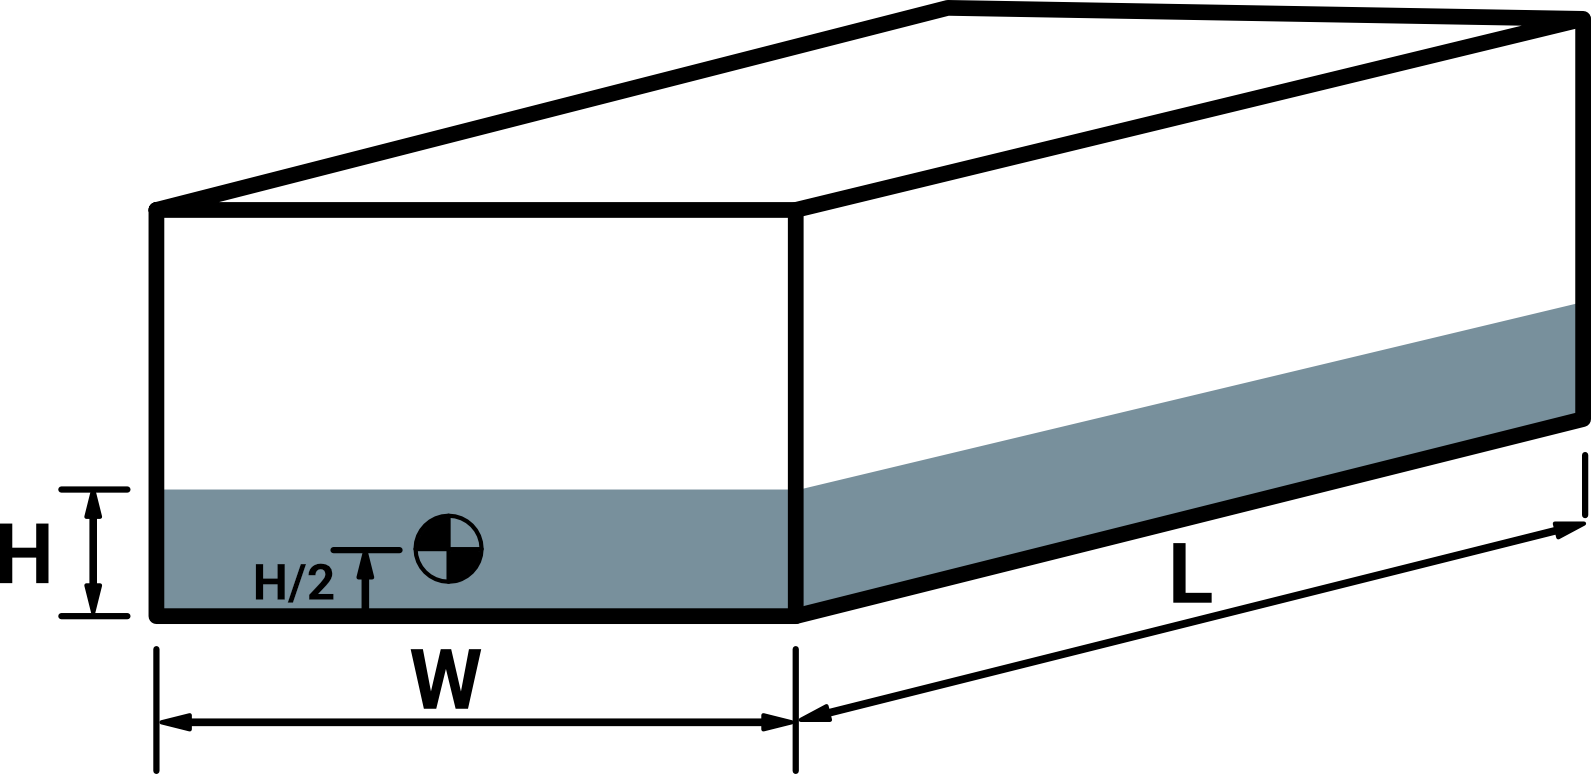
\includegraphics[width=0.5\textwidth]{fig/jad_payload_cgz_min}
	\caption{Minimum payload \gls{cgz} height}
	\label{figure:minimum-payload-cgz-height}
\end{figure}
%----------------------------------------------
%      FIGURE
%----------------------------------------------

The calculations of the minimum \gls{cgz} for each vehicle unit are summarised in Table~\ref{table:minimum-cgz-for-the-payload}.

%----------------------------------------------
%      TABLE - UPDATED TO NEW RANGES
%----------------------------------------------
\begin{table}[H]
	\centering\footnotesize
	\begin{threeparttable}

		\begin{tabulary}{\textwidth}{lCCCCCCc}
			\toprule
			\textbf{Combination} & \textbf{Width (m)} & \textbf{Length (m)} & \textbf{Payload density (kg/m\ssth)} & \textbf{Payload mass (kg)} & \textbf{H/2 (mm)} & \textbf{Deck height (mm)} & \textbf{Min. \gls{cgz}\tnote{1} (mm)} \\
			\midrule
            Rigid truck & 2.600   & 6.289 & 8050  & 14140 & 54 & 1068 & 1122\\
			Quad semi-trailer & 2.600   & 14.900 & 8050  & 32300 & 52 & 1528 & 1580\\
			Tridem interlink leader & 2.600   & 7.940 & 8050  & 24615 & 74 & 1593 & 1667\\
			Tridem interlink follower & 2.600   & 7.940 & 8050  & 24615 & 74 & 1593 &  1667\\
			Tridem semi-trailer & 2.600   & 12.456 & 8050  & 37000 & 71 & 1300 &  1371\\
			\bottomrule
		\end{tabulary}

		\caption{Minimum \gls{cgz} for the payload}
		\label{table:minimum-cgz-for-the-payload}

		\begin{tablenotes}
		\item[1] Measured from the ground
		\end{tablenotes}

	\end{threeparttable}
\end{table}
%----------------------------------------------
%      TABLE
%----------------------------------------------

The maximum payload \gls{cgz} height was determined from the geometrical location of the centre of gravity for a trapezoid with sides sloped at 20\degree{} according to Equation~\ref{equation:maximum-cgz-height}. This represents the payload distribution of a side-tipper filled to the top with payload which is typical for the transport of payloads with low densities.

%----------------------------------------------
%      EQUATION
%----------------------------------------------
\begin{align}
	\label{equation:maximum-cgz-height}
	y = h  \left ( 1 - \frac{1}{3} \times \frac{(b+2a)}{(b+a)} \right )
\end{align}

Where: $y$, $h$, $b$, and $a$ are the dimensions of the trapezoid as illustrated in Figure~\ref{figure:maximum-payload-cgz-height}.
%----------------------------------------------
%      EQUATION
%----------------------------------------------

%----------------------------------------------
%      FIGURE
%----------------------------------------------
\begin{figure}[H]
	\centering
	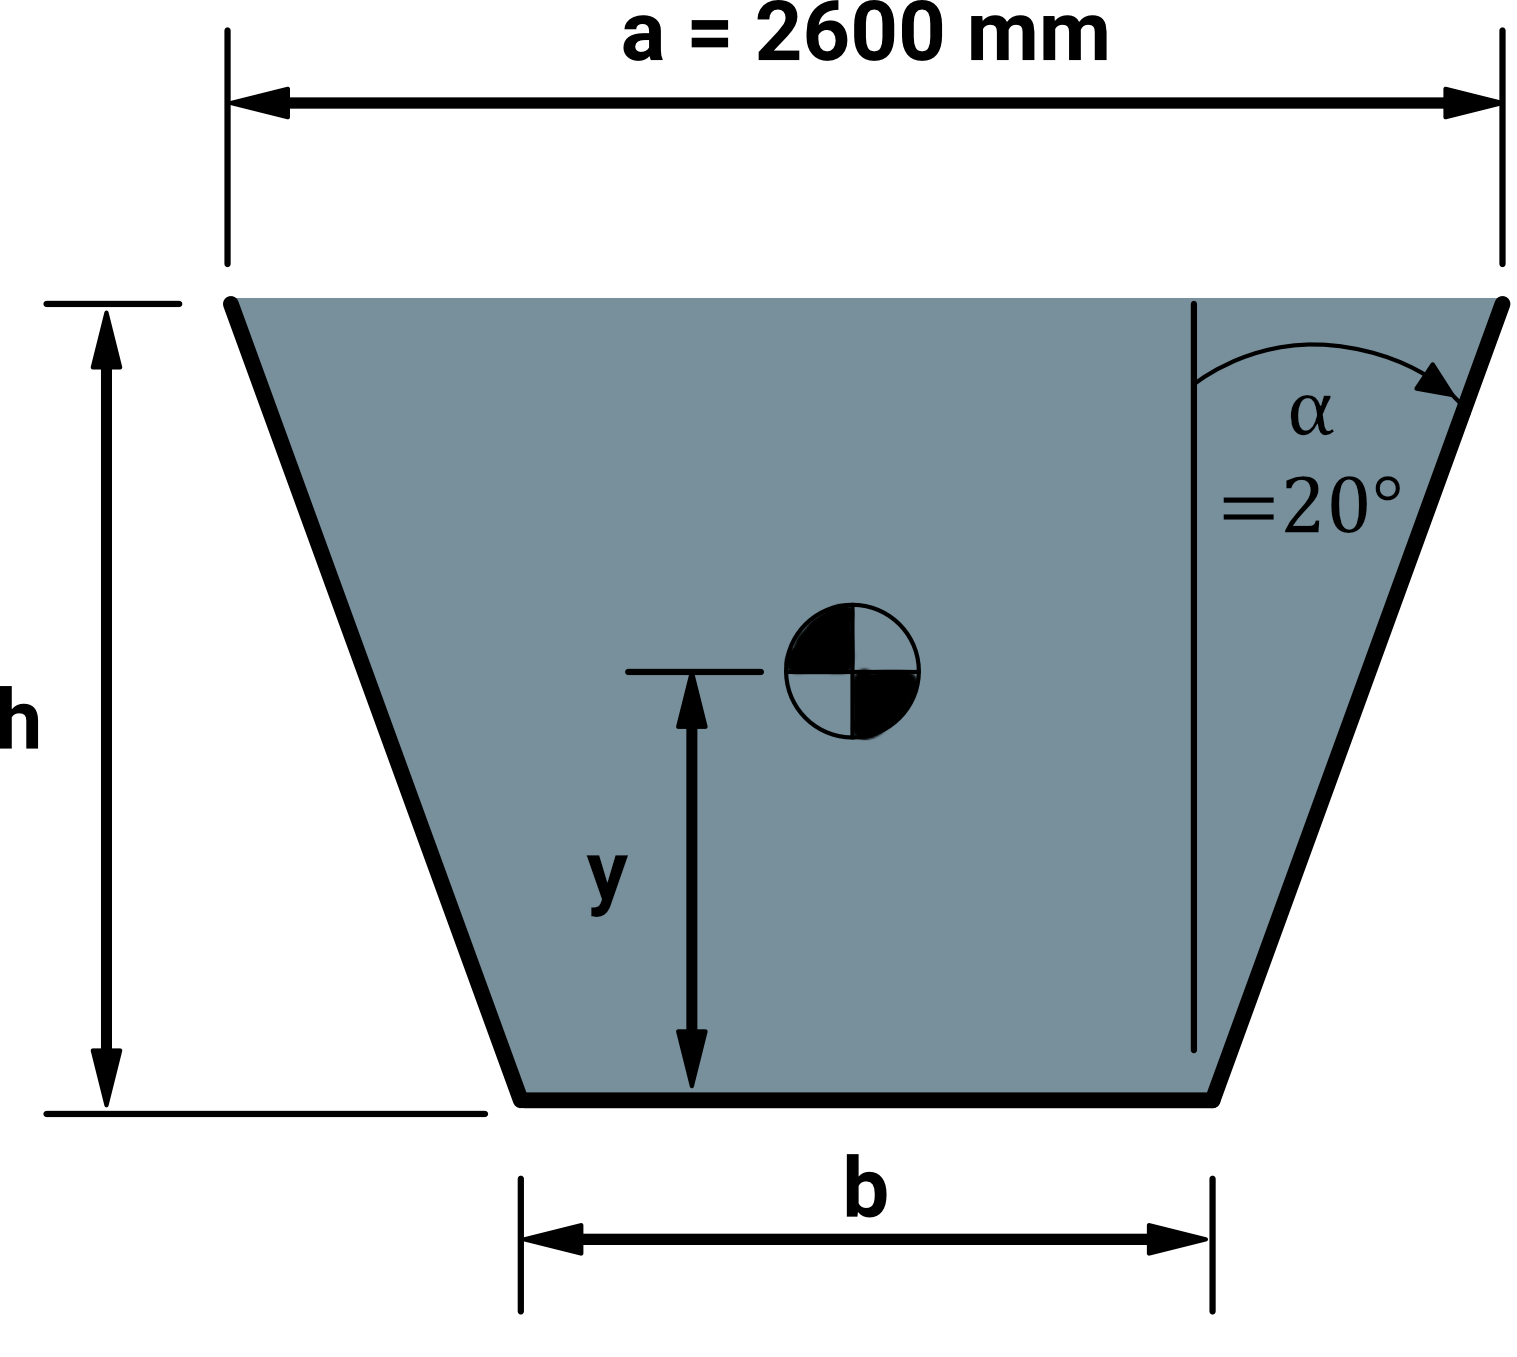
\includegraphics[width=0.5\textwidth]{fig/jad_payload_cgz_max}
	\caption{Maximum payload \gls{cgz} height}
	\label{figure:maximum-payload-cgz-height}
\end{figure}
%----------------------------------------------
%      FIGURE
%----------------------------------------------

The calculations for the maximum \gls{cgz} above ground are summarised in Table~\ref{table:payload-estimate-of-maximum-cgz-above-ground}.

%----------------------------------------------
%      TABLE - UPDATED TO NEW RANGES
%----------------------------------------------
\begin{table}[H]
	\centering\footnotesize
	\begin{threeparttable}

		\begin{tabulary}{\textwidth}{lccccC}
			\toprule
			\textbf{Combination} & \textbf{h (mm)} & \textbf{b (mm)} & \textbf{y (mm)} & \textbf{Deck height (mm)\tnote{1}} & \textbf{Max. \gls{cgz} (mm)\tnote{1}} \\

			\midrule
            Rigid truck & 3046  & 383   & 1900  & 1068  & 2968 \\
			Quad semi-trailer & 2272  & 946   & 1313  & 1528  & 2841 \\
			Tridem interlink leader & 1605  & 1432  & 880   & 1593  & 2473 \\
			Tridem interlink follower & 1605  & 383   & 880   & 1593  & 2473 \\
			Tridem semi-trailer & 2814  & 552   & 1712  & 1300  & 3012 \\
			\bottomrule
		\end{tabulary}

		\caption{Calculation of the maximum \gls{cgz} above ground}
		\label{table:payload-estimate-of-maximum-cgz-above-ground}

		\begin{tablenotes}
			\item[1] Measured from the ground
		\end{tablenotes}

	\end{threeparttable}
\end{table}
%----------------------------------------------
%      TABLE
%----------------------------------------------

%      SUBSECTION
%----------------------------------------------
\subsection{Payload Roll Moment of Inertia}\label{section:pr-roll-radius-of-gyration-payload}

The payload roll moment of inertia was assumed to vary according to the roll radius of gyration by an additional 5\% variation in comparison to the trailer vehicle units (see Section~\ref{section:pr-roll-moment-of-inertia-trailer-vehicle-units})  to account for the fact that payload geometry has additional scope to vary.

\begin{itemize}
\item \textbf{Payload \gls{rx} variation:} +/-50\%.
\end{itemize}

%      SUBSECTION
%----------------------------------------------
\subsection{Payload Pitch and Yaw Moment of Inertia}\label{section:pr-pitch-yaw-radius-of-gyration-payload}

There is additional scope for the pitch and yaw moment of inertia to vary relative to the roll moment of inertia. Thus, the payload pitch and yaw moment of inertia was assumed to vary according to the pitch and yaw radius of gyration by an additional 10\% in comparison to the trailer vehicle units unit (see Section~\ref{section:pr-pitch-yaw-radius-of-gyration-vehicle-units}) to account for the fact that payload has additional scope to vary.

\begin{itemize}
\item \textbf{Payload \gls{ry} and \gls{rz} variation:} +/-60\%.
\end{itemize}

%==============================================
%      SECTION
%==============================================
\section{Suspension Parameter Limits}\label{section:pr-suspension-parameter-limits}

The suspension parameter limits are often difficult to acquire from \glspl{oem}. Local distributors require permission from overseas design offices to release the proprietary information. Additionally, non-disclosures need to be signed when receiving technical information which can delay the data acquisition process.

To develop the evaluated ranges of the suspension parameter limits, existing literature was consulted for methods of estimating parameters and publicly available \gls{oem} datasheets were used to determine representative design parameters.

For some suspension parameters, data collected from \gls{pbs} assessments completed by \gls{wits} was used to investigate reasonable ranges. This data is protected by non-disclosure agreements and cannot be publicly disclosed in this dissertation. However variations in parameter values is presented relative to the baseline models.

A collection of measured vehicle design parameters is contained in studies such as those conducted by Fancher et al. \cite{Fancher1986} , \cite{Fancher1987}, Ervin et al. \cite{Ervin1986} and Harwood et al. \cite{Harwood2003}. These studies were conducted in the USA and Canada and may not be representative of the South African heavy vehicle fleet. These sources were used due to the lack of similar studies related to South African vehicles.

\subsection{Unsprung Mass}\label{section:pr-axle-unsprung-mass}

\textbf{Prime mover:} The unsprung masses recorded by Fancher et al. \cite{Fancher1986} for steer and drive axles as shown in Table~\ref{table:measured-unsprung-masses-fancher-et-al} are significantly lower than those generally observed in more modern prime movers. Therefore these were conservatively used as the minimum. The maximum steer and drive axle unsprung masses were determined from South African \gls{pbs} assessments and are included in Table \ref{table:pr-axle-unsprung-mass}.

%----------------------------------------------
%      TABLE
%----------------------------------------------
\begin{table}[H]
	\centering\footnotesize
	\begin{threeparttable}

		\begin{tabulary}{\textwidth}{lcc}
			\toprule
			\textbf{Axle type} & \textbf{Minimum (kg)} & \textbf{Maximum (kg)} \\
			\midrule
			Steer & \multicolumn{2}{c}{544}\\
			Drive & 1043  & 1134 \\
			Trailer & \multicolumn{2}{c}{798}\\
			\bottomrule
		\end{tabulary}

		\caption{Measured unsprung mass for steer, drive and trailer axles - Fancher et al. \cite{Fancher1986}}
		\label{table:measured-unsprung-masses-fancher-et-al}

		%\begin{tablenotes}
		%\item[1] %\tnote{1}
		%\end{tablenotes}

	\end{threeparttable}
\end{table}
%----------------------------------------------
%      TABLE
%----------------------------------------------

The range of unsprung masses for the trailer axles was determined from a collection of \gls{oem} data,  weights of generic suspension components collected from previous on-site measurements and South African \gls{pbs} assessments. 

To determine the minimum unsprung mass, data from the BPW axle catalogue was consolidated (see Tables~\ref{table:bpw-rigid-axles-with-300-mm-drum-brake}~to~\ref{table:bpw-rigid-axles-with-430-mm-disc-brake} included in Appendix \ref{section:bpw-rigid-axles-catalogue}). 

The minimum axle unpsrung mass was determined by combining the lightest BPW axle was with aluminium rims. The results of these calculations are summarised in Tables~\ref{table:unsprung-axle-mass-trailer-445-65-R22.5-singles-min}~to~\ref{table:unsprung-axle-mass-trailer-285-70-R19.5-duals-min}. 

The maximum trailer unsprung mass for each axle was determined from South African \gls{pbs} assessments since these were found to be heavier than the combination of the heaviest BPW axle with steel rims. The range of evaluated unsprung masses is summarised in Table~\ref{table:pr-axle-unsprung-mass}.

%----------------------------------------------
%      TABLE
%----------------------------------------------
\begin{table}[H]
	\centering\footnotesize
	\begin{threeparttable}

		\begin{tabulary}{\textwidth}{rrrrc}
			\toprule
			\multicolumn{1}{l}{\textbf{Component}} & \multicolumn{1}{c}{\textbf{Description}} & \multicolumn{1}{c}{\textbf{Quantity}} & \multicolumn{1}{c}{\textbf{Unit mass (kg)}} & \textbf{Total mass (kg)} \\
			\midrule
			\multicolumn{1}{l}{Tyre} & \multicolumn{1}{c}{445/65 R22.5} & \multicolumn{1}{c}{2} & \multicolumn{1}{c}{103.0} & 206.0 \\
			\multicolumn{1}{l}{Rim} & \multicolumn{1}{c}{Aluminium - 13"} & \multicolumn{1}{c}{2} & \multicolumn{1}{c}{26.5} & 53.0 \\
			\multicolumn{1}{l}{Axle} & \multicolumn{1}{c}{SKHSF 9010 (singles)} & \multicolumn{1}{c}{1} & \multicolumn{1}{c}{265.0} & 265.0 \\
			\multicolumn{1}{l}{Spring} & \multicolumn{1}{c}{Generic} & \multicolumn{1}{c}{2} & \multicolumn{1}{c}{5.6} & 11.2 \\
			\multicolumn{1}{l}{Damper} & \multicolumn{1}{c}{Generic} & \multicolumn{1}{c}{2} & \multicolumn{1}{c}{5.0} & 10.0 \\
            \midrule
			\multicolumn{4}{r}{\textbf{Total}} & 545.2 \\
			\bottomrule
		\end{tabulary}

		\caption{Minimum unsprung mass for a trailer axle with 445/65 R22.5 singles}
		\label{table:unsprung-axle-mass-trailer-445-65-R22.5-singles-min}

		%\begin{tablenotes}
		%\item[1] %\tnote{1}
		%\end{tablenotes}

	\end{threeparttable}
\end{table}
%----------------------------------------------
%      TABLE
%----------------------------------------------

%----------------------------------------------
%      TABLE
%----------------------------------------------
\begin{table}[H]
	\centering\footnotesize
	\begin{threeparttable}

		\begin{tabulary}{\textwidth}{rrrrc}
			\toprule
			\multicolumn{1}{l}{\textbf{Component}} & \multicolumn{1}{c}{\textbf{Description}} & \multicolumn{1}{c}{\textbf{Quantity}} & \multicolumn{1}{c}{\textbf{Unit mass (kg)}} & \textbf{Total mass (kg)} \\
			\midrule
			\multicolumn{1}{l}{Tyre} & \multicolumn{1}{c}{315/80 R22.5} & \multicolumn{1}{c}{4} & \multicolumn{1}{c}{68.7} & 274.8 \\
			\multicolumn{1}{l}{Rim} & \multicolumn{1}{c}{Aluminium - 9"} & \multicolumn{1}{c}{4} & \multicolumn{1}{c}{22.6} & 90.6 \\
			\multicolumn{1}{l}{Axle} & \multicolumn{1}{c}{SKHZF 9010 (duals)} & \multicolumn{1}{c}{1} & \multicolumn{1}{c}{280.0} & 280.0 \\
			\multicolumn{1}{l}{Spring} & \multicolumn{1}{c}{Generic} & \multicolumn{1}{c}{2} & \multicolumn{1}{c}{5.6} & 11.2 \\
			\multicolumn{1}{l}{Damper} & \multicolumn{1}{c}{Generic} & \multicolumn{1}{c}{2} & \multicolumn{1}{c}{5.0} & 10.0 \\
            \midrule
			\multicolumn{4}{r}{\textbf{Total}} & 666.5 \\
			\bottomrule
		\end{tabulary}

		\caption{Minimum unsprung mass for a trailer axle with 315/80 R22.5 duals}
		\label{table:unsprung-axle-mass-trailer-315-80-R22.5-duals-min}

		%\begin{tablenotes}
		%\item[1] %\tnote{1}
		%\end{tablenotes}

	\end{threeparttable}
\end{table}
%----------------------------------------------
%      TABLE
%----------------------------------------------

%----------------------------------------------
%      TABLE
%----------------------------------------------
\begin{table}[H]
	\centering\footnotesize
	\begin{threeparttable}

		\begin{tabulary}{\textwidth}{rrrrc}
			\toprule
			\multicolumn{1}{l}{\textbf{Component}} & \multicolumn{1}{c}{\textbf{Description}} & \multicolumn{1}{c}{\textbf{Quantity}} & \multicolumn{1}{c}{\textbf{Unit mass (kg)}} & \textbf{Total mass (kg)} \\
			\midrule
			\multicolumn{1}{l}{Tyre} & \multicolumn{1}{c}{285/70 R19.5} & \multicolumn{1}{c}{4} & \multicolumn{1}{c}{41.0} & 164.0 \\
			\multicolumn{1}{l}{Rim} & \multicolumn{1}{c}{Aluminium - 7.5"} & \multicolumn{1}{c}{4} & \multicolumn{1}{c}{18.7} & 74.7 \\
			\multicolumn{1}{l}{Axle} & \multicolumn{1}{c}{SKHZF 9008 (duals)} & \multicolumn{1}{c}{1} & \multicolumn{1}{c}{270.0} & 270.0 \\
			\multicolumn{1}{l}{Spring} & \multicolumn{1}{c}{Generic} & \multicolumn{1}{c}{2} & \multicolumn{1}{c}{5.6} & 11.2 \\
			\multicolumn{1}{l}{Damper} & \multicolumn{1}{c}{Generic} & \multicolumn{1}{c}{2} & \multicolumn{1}{c}{5.0} & 10.0 \\
            \midrule
			\multicolumn{4}{r}{\textbf{Total}} & 529.8 \\

			\bottomrule
		\end{tabulary}

		\caption{Minimum unsprung mass for a trailer axle with 285/70 R19.5 duals}
		\label{table:unsprung-axle-mass-trailer-285-70-R19.5-duals-min}

		%\begin{tablenotes}
		%\item[1] %\tnote{1}
		%\end{tablenotes}

	\end{threeparttable}
\end{table}
%----------------------------------------------
%      TABLE
%----------------------------------------------

%----------------------------------------------
%      TABLE - UPDATED TO NEW RANGES
%----------------------------------------------
\begin{table}[H]
	\centering\footnotesize
	\begin{threeparttable}

		\begin{tabulary}{\textwidth}{lccc}
			\toprule
			\textbf{Axle} & \textbf{Baseline (kg)} & \textbf{Min (kg)} & \textbf{Max (kg)} \\
			\midrule
			Steer & 750   & 544   & 800 \\
			Drive & 1300  & 1043   & 1350 \\
			Trailer (445/65 R22.5 - singles) & 760   & 545   & 800 \\
			Trailer (315/80 R22.5 - duals) & 900   & 667   & 1000 \\
			Trailer (285/70 R19.5 - duals) & 757   & 530   & 850 \\
			\bottomrule
		\end{tabulary}

		\caption{Parameter range - axle unsprung mass}
		\label{table:pr-axle-unsprung-mass}

		%\begin{tablenotes}
		%\item[1] %\tnote{1}
		%\end{tablenotes}

	\end{threeparttable}
\end{table}
%----------------------------------------------
%      TABLE
%----------------------------------------------

\subsection{Axle Roll and Yaw Moment of Inertia}\label{section:pr-axle-roll-yaw-inertia}
According to Winkler et al. \cite{Winkler2011}, the axle roll and yaw moment of inertia (\gls{ixx}/\gls{izz}) for steer, drive and trailer axles can be estimated with the range of radii of gyration provided in Table~\ref{table:estimated roll/yaw radius of gyrations for axles}. The axle \gls{rx} and \gls{rz} are approximately equal and are thus treated as a single \gls{vdp}.

%----------------------------------------------
%      TABLE
%----------------------------------------------
\begin{table}[H]
	\centering\footnotesize
	\begin{threeparttable}

		\begin{tabulary}{\textwidth}{lcc}
			\toprule
			\textbf{Axle type} & \textbf{Min. \gls{rx}/\gls{rz} (mm)} & \textbf{Max. \gls{rx}/\gls{rz} (mm)} \\
			\midrule
			Steer & 840 & 910\\
			Drive & 690 & 740\\
			Trailer & 790 & 860 \\
			\bottomrule
		\end{tabulary}

		\caption{Estimation range for axle \gls{rx}/\gls{rz} \cite{Winkler2011}}
		\label{table:estimated roll/yaw radius of gyrations for axles}

		%\begin{tablenotes}
		%\item[1] %\tnote{1}
		%\end{tablenotes}

	\end{threeparttable}
\end{table}
%----------------------------------------------
%      TABLE
%----------------------------------------------

The minimum and maximum axle roll and yaw inertias were determined using the baseline axle unsprung mass with the minimum and maximum axle roll and yaw radii of gyrations from Winkler et al. (see Table~\ref{table:estimated roll/yaw radius of gyrations for axles}).

The resulting range of axle roll and yaw inertia for each baseline axle is provided in Table~\ref{table:parameter-range-axle-roll-and-yaw-inertia}.

%----------------------------------------------
%      TABLE - UPDATED TO NEW RANGES
%----------------------------------------------
\begin{table}[H]
	\centering\footnotesize
	\begin{threeparttable}

		\begin{tabulary}{\textwidth}{lccc}
			\toprule
			\textbf{Axle} & \textbf{Baseline (kg.m\sstw)} & \textbf{Min. (kg.m\sstw)} & \textbf{Max. (kg.m\sstw)} \\
			\midrule
             Steer & 529   & 529   & 621 \\
             Drive & 619   & 619   & 712 \\
             Trailer (445/65 R22.5 singles)  & 474   & 474   & 562 \\
             Trailer (315/80 R22.5 duals) & 562   & 562   & 666 \\
             Trailer (285/70R22.5 duals) & 472   & 472   & 560 \\
			\bottomrule
		\end{tabulary}

		\caption{Parameter range - axle roll and yaw moment of inertia}
		\label{table:parameter-range-axle-roll-and-yaw-inertia}

		%\begin{tablenotes}
		%\item[1] %\tnote{1}
		%\end{tablenotes}

	\end{threeparttable}
\end{table}
%----------------------------------------------
%      TABLE
%----------------------------------------------

%      SUBSECTION
%----------------------------------------------
\subsection{Axle Spin Moment of Inertia}\label{section:pr-axle-spin-moment-of-inertia}

The spin inertia of the rotating components of the axle is generally quite small. A value of 2~kg.m\sstw{} was derived by de Saxe \cite{DeSaxe2012} from measured data published by Winkler et al. \cite{Winkler1995} which was considered the minimum value. The \trucksim{} 2018 database includes spin inertias of up to 20~kg.m\sstw{} (\textit{18t Trailer, Dual Wheels}) which was deemed reasonable as the maximum value for the spin inertia of the rotating axle components.

%      SUBSECTION
%----------------------------------------------
\subsection{Damper Dynamic Response}\label{section:pr-axle-damper}

Linear damping models in the \trucksim{} 2018 database range from 2.5~kN-s/m to 50~kN-s/m. Due to the complex nature of comparing the damping characteristics of non-linear damping, the effectiveness of which is dependent on the range of operation, the baseline damping was linearised and the damping was varied from 2.5~to~50~kN-s/m.

%      SUBSECTION
%----------------------------------------------
\subsection{Roll Steer Coefficient}\label{section:pr-roll-steer}

\gls{rollsteer} is the tendency for a non-steered rigid axle to exhibit some level of steering as an axle rolls relative to the vehicles sprung mass such as when travelling over a disturbance or when performing certain turning manoeuvres. An exaggerated illustration of this effect is shown in Figure~\ref{figure:Illustration-of-the-roll-steer-effect-on-a-rigid-axle}.

%----------------------------------------------
%      FIGURE
%----------------------------------------------
\begin{figure}[!htbp]
	\centering
	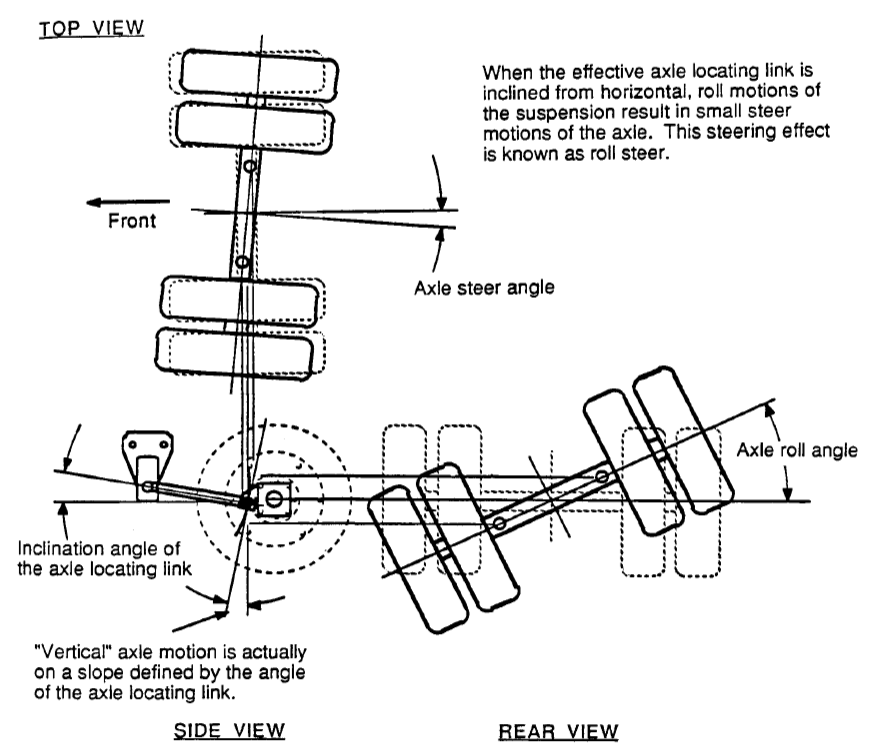
\includegraphics[width=1\textwidth]{fig/fancher-1986_roll-steer-illustration}
	\caption{Illustration of the roll steer effect on a rigid axle \cite{Fancher1986}}
	\label{figure:Illustration-of-the-roll-steer-effect-on-a-rigid-axle}
\end{figure}
%----------------------------------------------
%      FIGURE
%----------------------------------------------

Studies conducted by both Fancher et al. \cite{Fancher1986} and Harwood et al. \cite{Harwood2003} have resulted in a collection of measured roll steer coefficients. A comparison of the data from these sources is included in Table~\ref{table:comparison-of-roll-steer-coefficients}\footnote{The data published is according to the ISO coordinate system with the Z-axis (vertical) positive down and steering to the right as positive. The \trucksim{} coordinate system makes use of the SAE up coordinate system with the Z-axis positive up and steering to the left as positive. The data in this table has been converted from the published values to the SAE up coordinate system}.

%----------------------------------------------
%      TABLE
%----------------------------------------------
\begin{table}[H]
	\centering\footnotesize
	\begin{threeparttable}

		\begin{tabulary}{\textwidth}{lcccc}
			\toprule
			& \multicolumn{2}{c}{\textbf{Fancher et al. \cite{Fancher1986}}} & \multicolumn{2}{c}{\textbf{Harwood et al. \cite{Harwood2003}}} \\\cline{2-5}
			\textbf{Suspension type} & \multicolumn{1}{l}{\textbf{Min.}} & \multicolumn{1}{l}{\textbf{Max.}} & \multicolumn{1}{l}{\textbf{Min.}} & \multicolumn{1}{l}{\textbf{Max.}} \\
			\midrule
			Air suspension & -0.01 & -0.225 & -0.01 & -0.23 \\
			Single-axle leaf spring & 0     & -0.08 & 0     & -0.07 \\
			Steer axle & 0     & -0.2  &   -    & - \\
			Walking beam & -0.175 & -0.21 & -0.16 & -0.21 \\
			4-spring suspensions & 0.04  & -0.22 & -0.23 & 0.04 \\
			\bottomrule
		\end{tabulary}

		\caption{Measured roll steer coefficients from published data}
		\label{table:comparison-of-roll-steer-coefficients}

		%\begin{tablenotes}
		%\item[1] %\tnote{1}
		%\end{tablenotes}

	\end{threeparttable}
\end{table}
%----------------------------------------------
%      TABLE
%----------------------------------------------

The minimum and maximum values for the roll steer coefficient from Table~\ref{table:comparison-of-roll-steer-coefficients} were chosen to evaluate the broadest range of roll steer on each of the axles. The resulting range of values evaluated is summarised in Table~\ref{table:parameter-range-roll-steer-coefficients}.

%----------------------------------------------
%      TABLE - UPDATED TO NEW RANGES
%----------------------------------------------
\begin{table}[H]
	\centering\footnotesize
	\begin{threeparttable}

		\begin{tabulary}{\textwidth}{lccc}
			\toprule
			\textbf{Axle} & \textbf{Baseline (\degree{}/\degree{})} & \textbf{Min. (\degree{}/\degree{})} & \textbf{Max. (\degree{}/\degree{})} \\
			\midrule
			Steer & -0.087 & 0     & -0.2 \\
			Drive & 0     & 0.04  & -0.23 \\
			Trailer (singles) & -0.035 & 0.04  & -0.23 \\
			Trailer (duals) & -0.156 & 0.04  & -0.23 \\
			\bottomrule
		\end{tabulary}

		\caption{Parameter range - roll steer coefficients}
		\label{table:parameter-range-roll-steer-coefficients}

		%\begin{tablenotes}
		%\item[1] %\tnote{1}
		%\end{tablenotes}

	\end{threeparttable}
\end{table}
%----------------------------------------------
%      TABLE
%----------------------------------------------

%      SUBSECTION
%----------------------------------------------
\subsection{Axle Track}\label{section:pr-axle-track}

At a Smart Truck Review Panel meeting held in 2017, it was passed that the overall axle track width on a \gls{pbs} vehicle may exceed the legal limit of 2600~mm up to 2650~mm (zero tolerance and including tyre bulge). This is to allow increased axle track and thus improved stability for \gls{pbs} combinations.

It would not be practical for prime mover manufacturers to modify their designs to consider the new relaxations since they would not be able to be used in conjunction with a legal vehicle. Thus, a maximum overall width of 2600~mm was evaluated for the steer and drive axle. To account for new trailer designs that may take advantage of this new relaxation, the maximum axle track was found using a maximum overall axle width of 2650~mm with the minimum tyre spacing as specified by Michelin in their tyre data book \cite{Michelin}.

\textbf{Maximum axle track conditions:}

\begin{enumerate}
	\item Overall width of 2600~mm for steer and drive axle and 2650~mm for trailer axles.
	\item The dual tyres were arranged to have the minimum spacing as recommended by Michelin \cite{Michelin}.
\end{enumerate}

\textbf{Minimum axle track conditions:}

No regulations were defined for minimum axle track width. A catalogue of rigid axles supplied by BPW (see Appendix~\ref{section:bpw-rigid-axles-catalogue}) \cite{BPW2010} was consulted to determine the minimum axle tracks available to avoid evaluation of unrepresentative narrow axle tracks. Only axles in the 9000 kg + rated load category were considered.

A selection of the BPW axles illustrating the variability of their axle tracks is provided in Table~\ref{table:bpw-axle-tracks}.

%----------------------------------------------
%      TABLE
%----------------------------------------------
\begin{table}[H]
	\centering\footnotesize
	\begin{threeparttable}

		\begin{tabulary}{\textwidth}{lccccc}
			\toprule
			\textbf{Axle Model} & \textbf{Tyre arrangement} & \textbf{Rim} & \textbf{Rated load (kg)} & \textbf{Min. (mm)} & \textbf{Max. (mm)} \\
			\midrule
			NHZF  & Duals & 19.5" & 9000  & 1830  & 1995 \\
			SHZF  & Duals & 22.5" & 9000-12000 & 1820  & 1880 \\
			SKHSF & Singles & 22.5" & 9000  & 2000  & 2140 \\
			\bottomrule
		\end{tabulary}

		%\begin{tablenotes}
		%\item[1] %\tnote{1}
		%\end{tablenotes}
        
        \caption{BPW axle tracks}
		\label{table:bpw-axle-tracks}

	\end{threeparttable}
\end{table}
%----------------------------------------------
%      TABLE
%----------------------------------------------

A limiting factor was the baseline spring and damper track, it was ensured that the edge of the tyres did not move past the spring or damper centre. In all cases, the minimum tracks from the BPW catalogue were suitable and did not cause interference with the spring or damper track.

In addition to the BPW axles, data collected from Fancher et al. \cite{Fancher1986} was used to consider alternative \glspl{oem} as well as ranges of steer axle track widths. A summary of the representative track widths is included in Table~\ref{table:measured-axle-track-widths-from-fancher-et-al}. The data from Fancher et al. is for American based vehicles with tractor widths of 96" (approx. 2439~mm) and trailer widths of 102" (approx. 2591~mm) which closely approximate the widths of local heavy vehicles. Thus, the axle track widths were deemed to be representative for vehicles operating within South Africa.

%----------------------------------------------
%      TABLE
%----------------------------------------------
\begin{table}[H]
	\centering\footnotesize
	\begin{threeparttable}

		\begin{tabulary}{\textwidth}{lcc}
			\toprule
			\textbf{Axle} & \textbf{Min. (mm)} & \textbf{Max. (mm)} \\
			\midrule
			Steer (96" cab width) & 1956  & 2057 \\
			Drive (96" cab width) & 1803  & 1829 \\
			Trailer (102" trailer width) & 1956  & 1981 \\
			\bottomrule
		\end{tabulary}

		\caption{Measured axle track widths from Fancher et al. \cite{Fancher1986}}
		\label{table:measured-axle-track-widths-from-fancher-et-al}

		%\begin{tablenotes}
		%\item[1] %\tnote{1}
		%\end{tablenotes}

	\end{threeparttable}
\end{table}
%----------------------------------------------
%      TABLE
%----------------------------------------------

Considering the worst-case minimum from either the BPW data book or Fancher et al. \cite{Fancher1986}, the range of axle tracks evaluated for each axle is included in Table~\ref{table:parameter-range-axle-track}.

%----------------------------------------------
%      TABLE - UPDATED TO NEW RANGES
%----------------------------------------------
\begin{table}[H]
	\centering\footnotesize
	\begin{threeparttable}

		\begin{tabulary}{\textwidth}{lccc}
			\toprule
             \textbf{Axle} & \textbf{Baseline (mm)} & \textbf{Min. (mm)} & \textbf{Max. (mm)} \\
			\midrule
             Steer & 2109  & 1950  & 2282 \\
             Drive & 1837  & 1800  & 1932 \\
             Trailer (445/65 R22.5 singles)  & 2140  & 2000  & 2178 \\
             Trailer (315/80 R22.5 duals) & 1920  & 1820  & 1982 \\
             Trailer (285/70R22.5 duals) & 2040  & 1830  & 2042 \\
			\bottomrule
		\end{tabulary}

		\caption{Parameter range - axle track width}
		\label{table:parameter-range-axle-track}

		%\begin{tablenotes}
		%\item[1] %\tnote{1}
		%\end{tablenotes}

	\end{threeparttable}
\end{table}
%----------------------------------------------
%      TABLE
%----------------------------------------------

\subsection{Spring and Damper Track}\label{section:spring and damper track}

The BPW axle catalogues \cite{BPW2010} (see Appendix~\ref{section:bpw-rigid-axles-catalogue}) were also used to develop the range of spring tracks. 

The minimum spring track from the BPW catalogues was chosen as the minimum for the trailer, drive and steer axles. The maximum BPW spring track was used as the maximum for the trailer axles. The maximum steer and drive axle tracks was limited by the baseline suspension geometry.

For all axles, it was assumed that the damper track could vary within the same range as the spring track. The resulting range of evaluated spring and damper tracks is summarised in Table~\ref{table:bpw-spring-and-damper-tracks}.

%----------------------------------------------
%      TABLE
%----------------------------------------------
\begin{table}[H]
	\centering\footnotesize
	\begin{threeparttable}

		\begin{tabulary}{\textwidth}{lccccc}
			\toprule
			\textbf{Axle} & \multicolumn{1}{l}{\textbf{Min. (mm)}} & \multicolumn{1}{l}{\textbf{Max. (mm)}} \\
			\midrule

			Steer & 780 & 1150 \\
			Drive & 670 & 1100 \\
			Trailer (single tyre) & 780 & 1500 \\
			Trailer (dual tyre) & 670 & 1200 \\
			\bottomrule
		\end{tabulary}

		%\begin{tablenotes}
		%\item[1] %\tnote{1}
		%\end{tablenotes}
        
        \caption{Parameter range - spring and damper track width}
		\label{table:bpw-spring-and-damper-tracks}

	\end{threeparttable}
\end{table}
%----------------------------------------------
%      TABLE
%----------------------------------------------


%      SUBSECTION
%----------------------------------------------
\subsection{Spring Vertical Stiffness}\label{section:pr-spring-stiffness}

The range of spring vertical stiffness values were determined from spring data collected from PBS assessments conducted by Wits University\footnote{\gls{oem} data protected by non-disclosure agreements and hence anonymised in this dissertation}.

The dynamic spring response for airbags is dependent on the vertical load. To compare the dynamic spring response, the response was linearly interpolated to a vertical load of 25000~N.

The results contained in Table \ref{table:comparison-of-dynamic-response-of-airbag-springs} indicate that there are significant variations (up to 186\%) in the spring stiffness between the different airbags at the static vertical load of 25000~N. It was assumed that any of the springs could be fitted to any of the axles to evaluate the full range of possibilities.

%----------------------------------------------
%      TABLE
%----------------------------------------------
\begin{table}[H]
	\centering\footnotesize
	\begin{threeparttable}
    
    	\caption{Comparison of the stiffness of airbag springs at 25000~N}
		\label{table:comparison-of-dynamic-response-of-airbag-springs}

		\begin{tabulary}{\textwidth}{lCCC}
			\toprule
			\textbf{Airbag type} & \textbf{Interpolated stiffness at 25000~N (N/mm)} & \textbf{Variation from drive axle baseline (\%)} & \textbf{Variation from trailer axle baseline (\%)} \\
			\midrule
			Trailer & 104   & 47\%  & 69\% \\
			Trailer & 205   & 92\%  & 137\% \\
			Drive & 94    & 42\%  & 62\% \\
			Steer & 157   & 71\%  & 105\% \\
			Drive & 115   & 52\%  & 77\% \\
			Drive & 155   & 70\%  & 103\% \\
			Drive & 270   & 121\% & 180\% \\
			Drive & 130   & 59\%  & 87\% \\
			Drive & 150   & 67\%  & 100\% \\
			Drive & 280   & 126\% & 186\% \\
			Drive & 100   & 45\%  & 67\% \\
			Drive & 122   & 55\%  & 82\% \\
			Drive & 222   & 100\% & 148\% \\
			Drive & 140   & 63\%  & 93\% \\
			Drive & 280   & 126\% & 186\% \\
			Trailer & 150   & 67\%  & 100\% \\
			Trailer & 151   & 68\%  & 100\% \\
			\bottomrule
		\end{tabulary}

		%\begin{tablenotes}
		%\item[1] %\tnote{1}
		%\end{tablenotes}

	\end{threeparttable}
\end{table}
%----------------------------------------------
%      TABLE
%----------------------------------------------

The baseline steer axles are fitted with a steel spring suspension. Sample steel spring stiffness values are provided in the \trucksim{} 2018 database that range from 200~N/mm to 350~N/mm. 350~N/mm was used as the maximum steel suspension stiffness. The minimum stiffness was evaluated as 185~N/mm according to the conservative spring stiffness used in the TERNZ \gls{srt} calculator \cite{TERNZTransportResearch} when a generic steer axle suspension is selected.

The resulting range of spring vertical stiffness values are provided in Table~\ref{table:parameter-range-spring-vertical-stiffness}. In the case of air springs, the baseline value is reported as 100\% of the baseline spring response, with the minimum and maximum variations scaled as a percentage of the baseline spring response.

%----------------------------------------------
%      TABLE
%----------------------------------------------
\begin{table}[H]
	\centering\footnotesize
	\begin{threeparttable}

		\begin{tabulary}{\textwidth}{lccc}
			\toprule
			\textbf{Axle} & \textbf{Baseline} & \textbf{Min.} & \textbf{Max.} \\
			\midrule
             Steer & 273 N/mm & 185 N/mm & 350 N/mm \\
             Drive & 100\% & 42\%  & 126\% \\
             Trailer & 100\% & 62\%  & 186\% \\
			\bottomrule
		\end{tabulary}

		\caption{Parameter range - spring vertical stiffness}
		\label{table:parameter-range-spring-vertical-stiffness}

		%\begin{tablenotes}
		%\item[1] %\tnote{1}
		%\end{tablenotes}

	\end{threeparttable}
\end{table}
%----------------------------------------------
%      TABLE
%----------------------------------------------

%      SUBSECTION
%----------------------------------------------
\subsection{Jounce and Rebound Stops}\label{section:pr-jounce-rebound-stops}

The jounce (upward movement) and rebound (downward movement) stops indicate the possible range of vertical movement for a suspension assembly as limited by mechanical constraints. Data collected from \gls{oem}s range from 45~mm to 110~mm up (jounce) and 50~mm to 120~mm down (rebound).

The \trucksim{} 2018 database includes jounce rebound stops of up to +250~mm / -250~mm. This is generally used as a conservative estimate in the case that an \gls{oem} does not supply sufficient information to determine jounce/rebound stops for the suspension. This was hence used as the worst case.

The lower end of the range was conservatively chosen from the \gls{oem} data with the upper end chosen from the \trucksim{} 2018 database due to the jounce and rebound stops rarely being supplied. 

To simplify the modelling, it was assumed that the jounce and rebound stops would be equal, resulting in the limits summarised in Table~\ref{table:parameter-jounce-and-rabound-stops} used for all baseline axles.

%----------------------------------------------
%      TABLE
%----------------------------------------------
\begin{table}[H]
	\centering\footnotesize
	\begin{threeparttable}

		\begin{tabulary}{\textwidth}{lccc}
			\toprule
			\textbf{Axle} & \textbf{Baseline} & \textbf{Min. (mm)} & \textbf{Max. (mm)} \\
			\midrule
			All & Varies & +45/-45 & +250/-250 \\
			\bottomrule
		\end{tabulary}

		\caption{Parameter range -  jounce and rebound stops}
		\label{table:parameter-jounce-and-rabound-stops}

		%\begin{tablenotes}
		%\item[1] %\tnote{1}
		%\end{tablenotes}

	\end{threeparttable}
\end{table}
%----------------------------------------------
%      TABLE
%----------------------------------------------

%      SUBSECTION
%----------------------------------------------
\subsection{Auxiliary Roll Stiffness}\label{section:pr-auxiliary-roll-stiffness}

To adhere to the \gls{pbs} requirement of a minimum \gls{srt} of 0.35~g, \gls{pbs} combinations are designed with higher auxiliary roll stiffness values to improve their rollover performance. Thus, the collected \gls{oem} data from South African \gls{pbs} assessments is skewed towards the suspensions with higher auxiliary roll stiffness. 

The \gls{oem} data is a good indicator of the upper end of auxiliary roll stiffness values while the data collected by Fu et al. \cite{Fu2002} from an analysis of several contemporary suspension designs is assumed to be a good indicator of the lower end of auxiliary roll stiffness values. 

A comparison of the ranges of auxiliary roll stiffness provided by \glspl{oem} is made with the data collected by Fu et al. in Table~\ref{table:comparison-of-auxiliary-roll-stiffness-ranges}. The resulting limits for auxiliary roll stiffness of each of the baseline axles is provided in Table \ref{table:parameter-range-auxiliary-roll-stiffness}.

%----------------------------------------------
%      TABLE - UPDATED TO NEW RANGES
%----------------------------------------------
\begin{table}[H]
	\centering\footnotesize
	\begin{threeparttable}

		\begin{tabulary}{\textwidth}{lCCCC}
			\toprule
			\textbf{Axle} & \makecell{\textbf{Min. (Nm/deg)} \\ \textbf{(OEM)}} & \makecell{\textbf{Max. (Nm/deg)} \\ \textbf{(OEM)}} & \makecell{\textbf{Min. (Nm/deg)} \\ \textbf{(Fu et al.)}} & \makecell{\textbf{Max. (Nm/deg)} \\ \textbf{(Fu et al.)}} \\
			\midrule
			Steer & 1850  & 5009  & 1070  & 1470 \\
			Drive & 7226  & 12689 & 790   & 2030 \\
			Trailer & 23736 & 35954 & 2260  & 13560 \\
			\bottomrule
		\end{tabulary}

		\caption{Comparison of auxiliary roll stiffness ranges from \glspl{oem} and Fu et al. \cite{Fu2002}}
		\label{table:comparison-of-auxiliary-roll-stiffness-ranges}

		%\begin{tablenotes}
		%\item[1] %\tnote{1}
		%\end{tablenotes}

	\end{threeparttable}
\end{table}
%----------------------------------------------
%      TABLE
%----------------------------------------------

%----------------------------------------------
%      TABLE - UPDATED TO NEW RANGES
%----------------------------------------------
\begin{table}[H]
	\centering\footnotesize
	\begin{threeparttable}

		\begin{tabulary}{\textwidth}{lccc}
			\toprule
			\textbf{Axle} & \textbf{Baseline} & \textbf{Min. (Nm/deg) (Fu et al.)} & \textbf{Max. (Nm/deg) (OEM)} \\
			\midrule
			Steer & 2950  & 1070  & 5009 \\
			Drive & 7487 & 790 & 12689 \\
			Trailer & 24700 & 2260  & 35954 \\
			\bottomrule
		\end{tabulary}

		\caption{Parameter range - auxiliary roll stiffness}
		\label{table:parameter-range-auxiliary-roll-stiffness}

		%\begin{tablenotes}
		%\item[1] %\tnote{1}
		%\end{tablenotes}

	\end{threeparttable}
\end{table}
%----------------------------------------------
%      TABLE
%----------------------------------------------

%      SUBSECTION
%----------------------------------------------
\subsection{Wheel and Axle Centre Height}\label{section:axle-centre-height}

The wheel centre height was assumed to vary from the laden height up to an increased height by half of the deflection between laden and unladen conditions (using the Michelin data book \cite{Michelin} for the unladen heights). These wheel centre height maximums are presented in Table~\ref{table:wheel-centre-height-variation-due-to-tyre-deflection}.

The height of the axle \gls{cg} is generally assumed equal to the wheel centre height since it is not supplied by the \glspl{oem} and detailed drawings (which tend to be proprietary) would be needed to determine the offset of the axle centre height relative to the wheel centre height.

The \trucksim{} 2018 database has a maximum axle centre offset relative to the wheel centre height of 60~mm (\textit{3t Drive, single wheels}). This was assumed to be the maximum offset above or below the wheel centre height resulting in the range of axle centre heights being evaluated as per Table \ref{table:parameter-range-wheel-and-axle-centre-height}.

%----------------------------------------------
%      TABLE - UPDATED TO NEW RANGES
%----------------------------------------------
\begin{table}[H]
	\centering\footnotesize
	\begin{threeparttable}

		\begin{tabulary}{\textwidth}{lcccC}
			\toprule
			\textbf{Tyre} & \makecell{\textbf{Laden radius} \\ \textbf{(mm)}} & \makecell{\textbf{Unladen radius} \\ \textbf{(mm)}} & \makecell{\textbf{Deflection} \\ \textbf{(mm)}} & \textbf{Max. wheel centre height (mm)}\\
			\midrule
            285/70 R19.5 & 413   & 456   & 42.50 & 434.3 \\
            315/80 R22.5 & 507   & 548   & 41.00 & 527.5 \\
            445/65 R22.5 & 534   & 587   & 53.00 & 560.5 \\
			\bottomrule
		\end{tabulary}

		\caption{Wheel centre height variation due to tyre deflection \cite{Michelin}}
		\label{table:wheel-centre-height-variation-due-to-tyre-deflection}

		%\begin{tablenotes}
		%\item[1] %\tnote{1}
		%\end{tablenotes}

	\end{threeparttable}
\end{table}
%----------------------------------------------
%      TABLE
%----------------------------------------------

%----------------------------------------------
%      TABLE - UPDATED TO NEW RANGES
%----------------------------------------------
\begin{table}[H]
	\centering\footnotesize
	\begin{threeparttable}

		\begin{tabulary}{\textwidth}{lccc}
			\toprule
			\textbf{Parameter} & \textbf{Baseline (mm)\tnote{1}} & \textbf{Min. (mm) } & \textbf{Max. (mm)}\\
			\midrule
            
            Wheel centre height (445/65 R22.5) & 534.0   & 534.0   & 560.5 \\
            Wheel centre height (315/80 R22.5) & 507.0  & 507.0   & 527.5 \\
            Wheel centre height (285/70 R19.5) & 413.0   & 413.0   & 434.3 \\          
            Axle centre height (445/65 R22.5) & 534.0   & 474.0   & 594.0 \\
            Axle centre height (315/80 R22.5) & 507.0   & 447.0   & 567.0 \\
            Axle centre height (285/70 R19.5) & 413.0   & 353.0  & 473.0 \\
            
			\bottomrule
		\end{tabulary}

		\caption{Parameter range - wheel and axle centre height}
		\label{table:parameter-range-wheel-and-axle-centre-height}

		\begin{tablenotes}
			\item[1] Height relative to the ground
		\end{tablenotes}

	\end{threeparttable}
\end{table}
%----------------------------------------------
%      TABLE
%----------------------------------------------

%      SUBSECTION
%----------------------------------------------
\subsection{Roll Centre Height}\label{section:pr-roll-centre-heights}

Winkler et al. \cite{Winkler2011} has documented a set of graphical methods for determining the roll centre based on the geometry of the suspension (see Figure~\ref{figure:estimate-of-roll-centre-heights-for-typical-suspension-configurations}). Using the graphical method for typical trailing arm suspensions, the maximum distance of the roll centre height from the centre of the axle is when the leaf spring makes an angle of 0\degree{} to the horizontal. Thus, the vertical distance from the centre of the lever arm to the centre of the axle will be a maximum when the thickness of the lever arm and cross-sectional height of the axle are at a maximum.

\begin{figure*}
	\centering
	\begin{subfigure}[t]{0.45\textwidth}
		\centering
		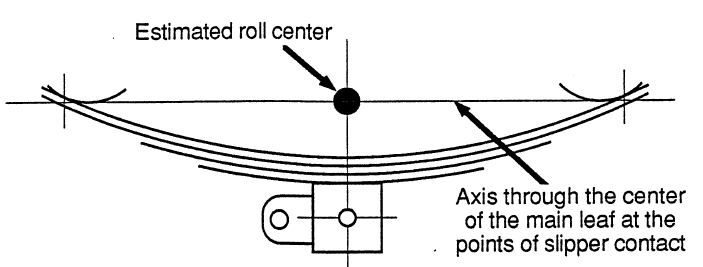
\includegraphics[height=1.2in]{fig/winkler-2011_roll-centre-estimation_typical-four-spring-suspensions}
		\caption{Typical four spring suspensions}
	\end{subfigure}%
	\hfill
	\begin{subfigure}[t]{0.45\textwidth}
		\centering
		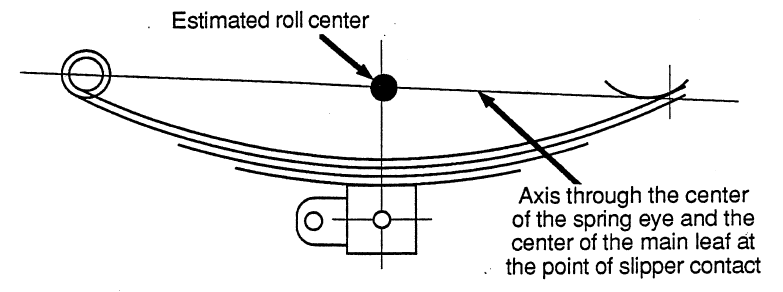
\includegraphics[height=1.2in]{fig/winkler-2011_roll-centre-estimation_typical-single-axle-rear-suspensions}
		\caption{Typical single axle rear suspensions}
	\end{subfigure}

	\begin{subfigure}[t]{0.45\textwidth}
		\centering
		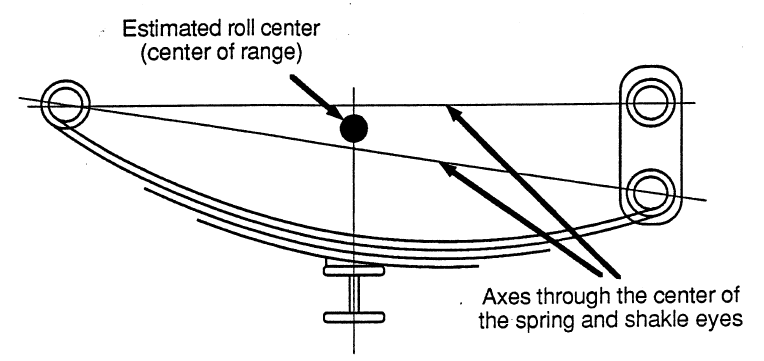
\includegraphics[height=1.2in]{fig/winkler-2011_roll-centre-estimation_typical-front-axle-suspensions}
		\caption{Typical front axle suspensions}
	\end{subfigure}
	\hfill
	\begin{subfigure}[t]{0.45\textwidth}
		\centering
		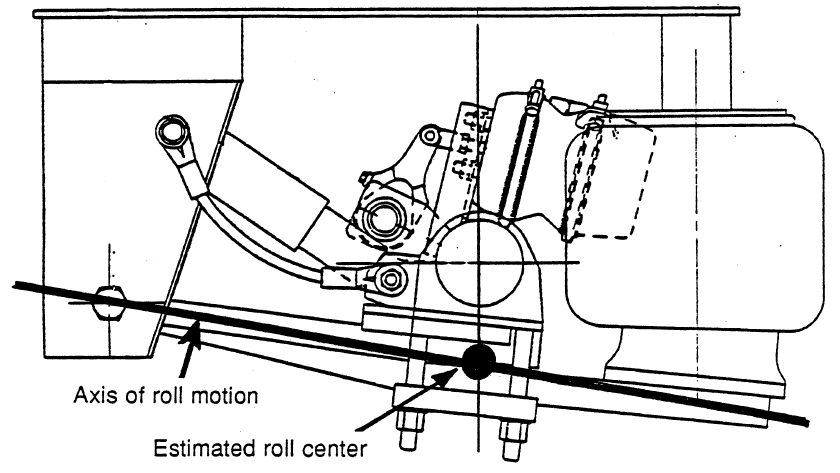
\includegraphics[height=1.2in]{fig/winkler-2011_roll-centre-estimation_compliant-trailing-arm-suspensions}
		\caption{Typical trailing arm suspensions}
	\end{subfigure}
	\caption{Estimate of roll centre heights for typical suspension configurations \cite{Winkler2011}}
	\label{figure:estimate-of-roll-centre-heights-for-typical-suspension-configurations}
\end{figure*}

The maximum axle cross section in the BPW rigid axles catalogue \cite{BPW2010} is 150~mm. Thus, assuming a maximum trailing arm thickness at the location of the axle of 100~mm to account for mounting plates, the maximum roll centre height from the centre of the axle is 125~mm below when the suspension is overslung and above when underslung as shown in Figure~\ref{figure:roll-centre-height-estimates-for-trailing-arm-suspension}.

%----------------------------------------------
%      FIGURE
%----------------------------------------------
\begin{figure*}[!htbp]
	\centering
	\begin{subfigure}[t]{0.45\textwidth}
		\centering
		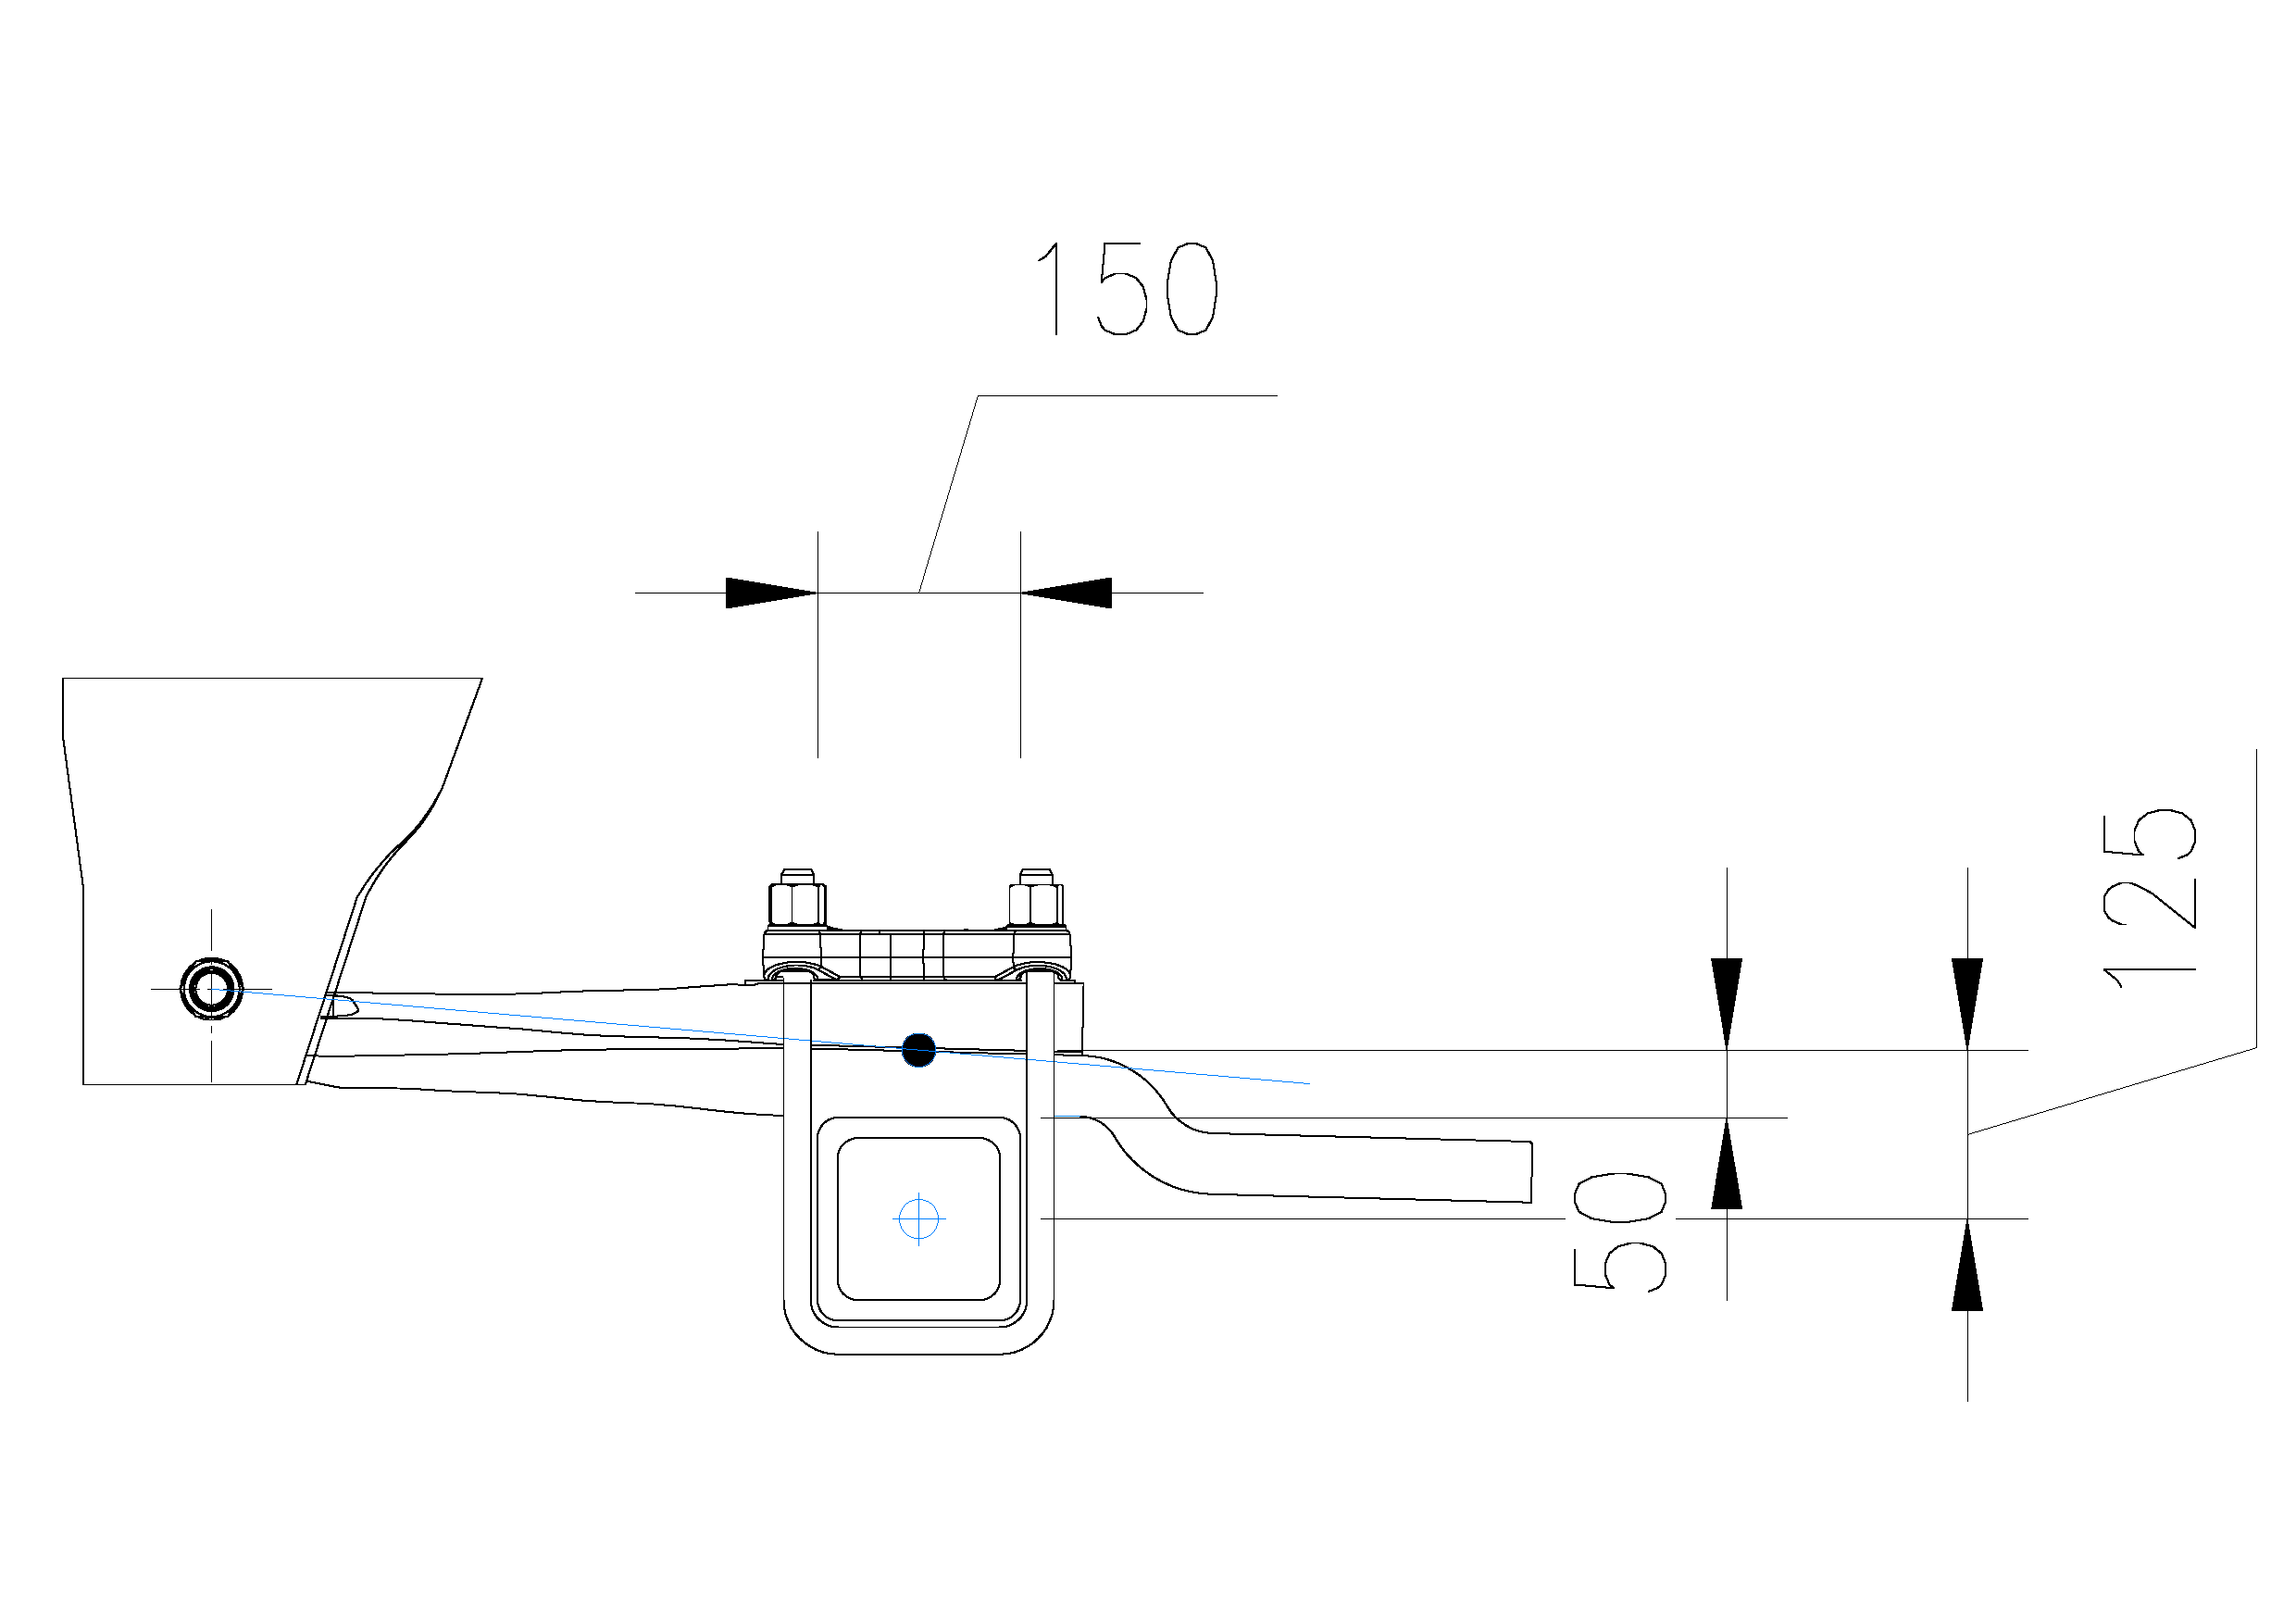
\includegraphics[width=1\textwidth]{fig/parameter-selection_roll-centre-height_overslung}
		\caption{Overslung (+125~mm)}
	\end{subfigure}\hfill
	\begin{subfigure}[t]{0.45\textwidth}
		\centering
		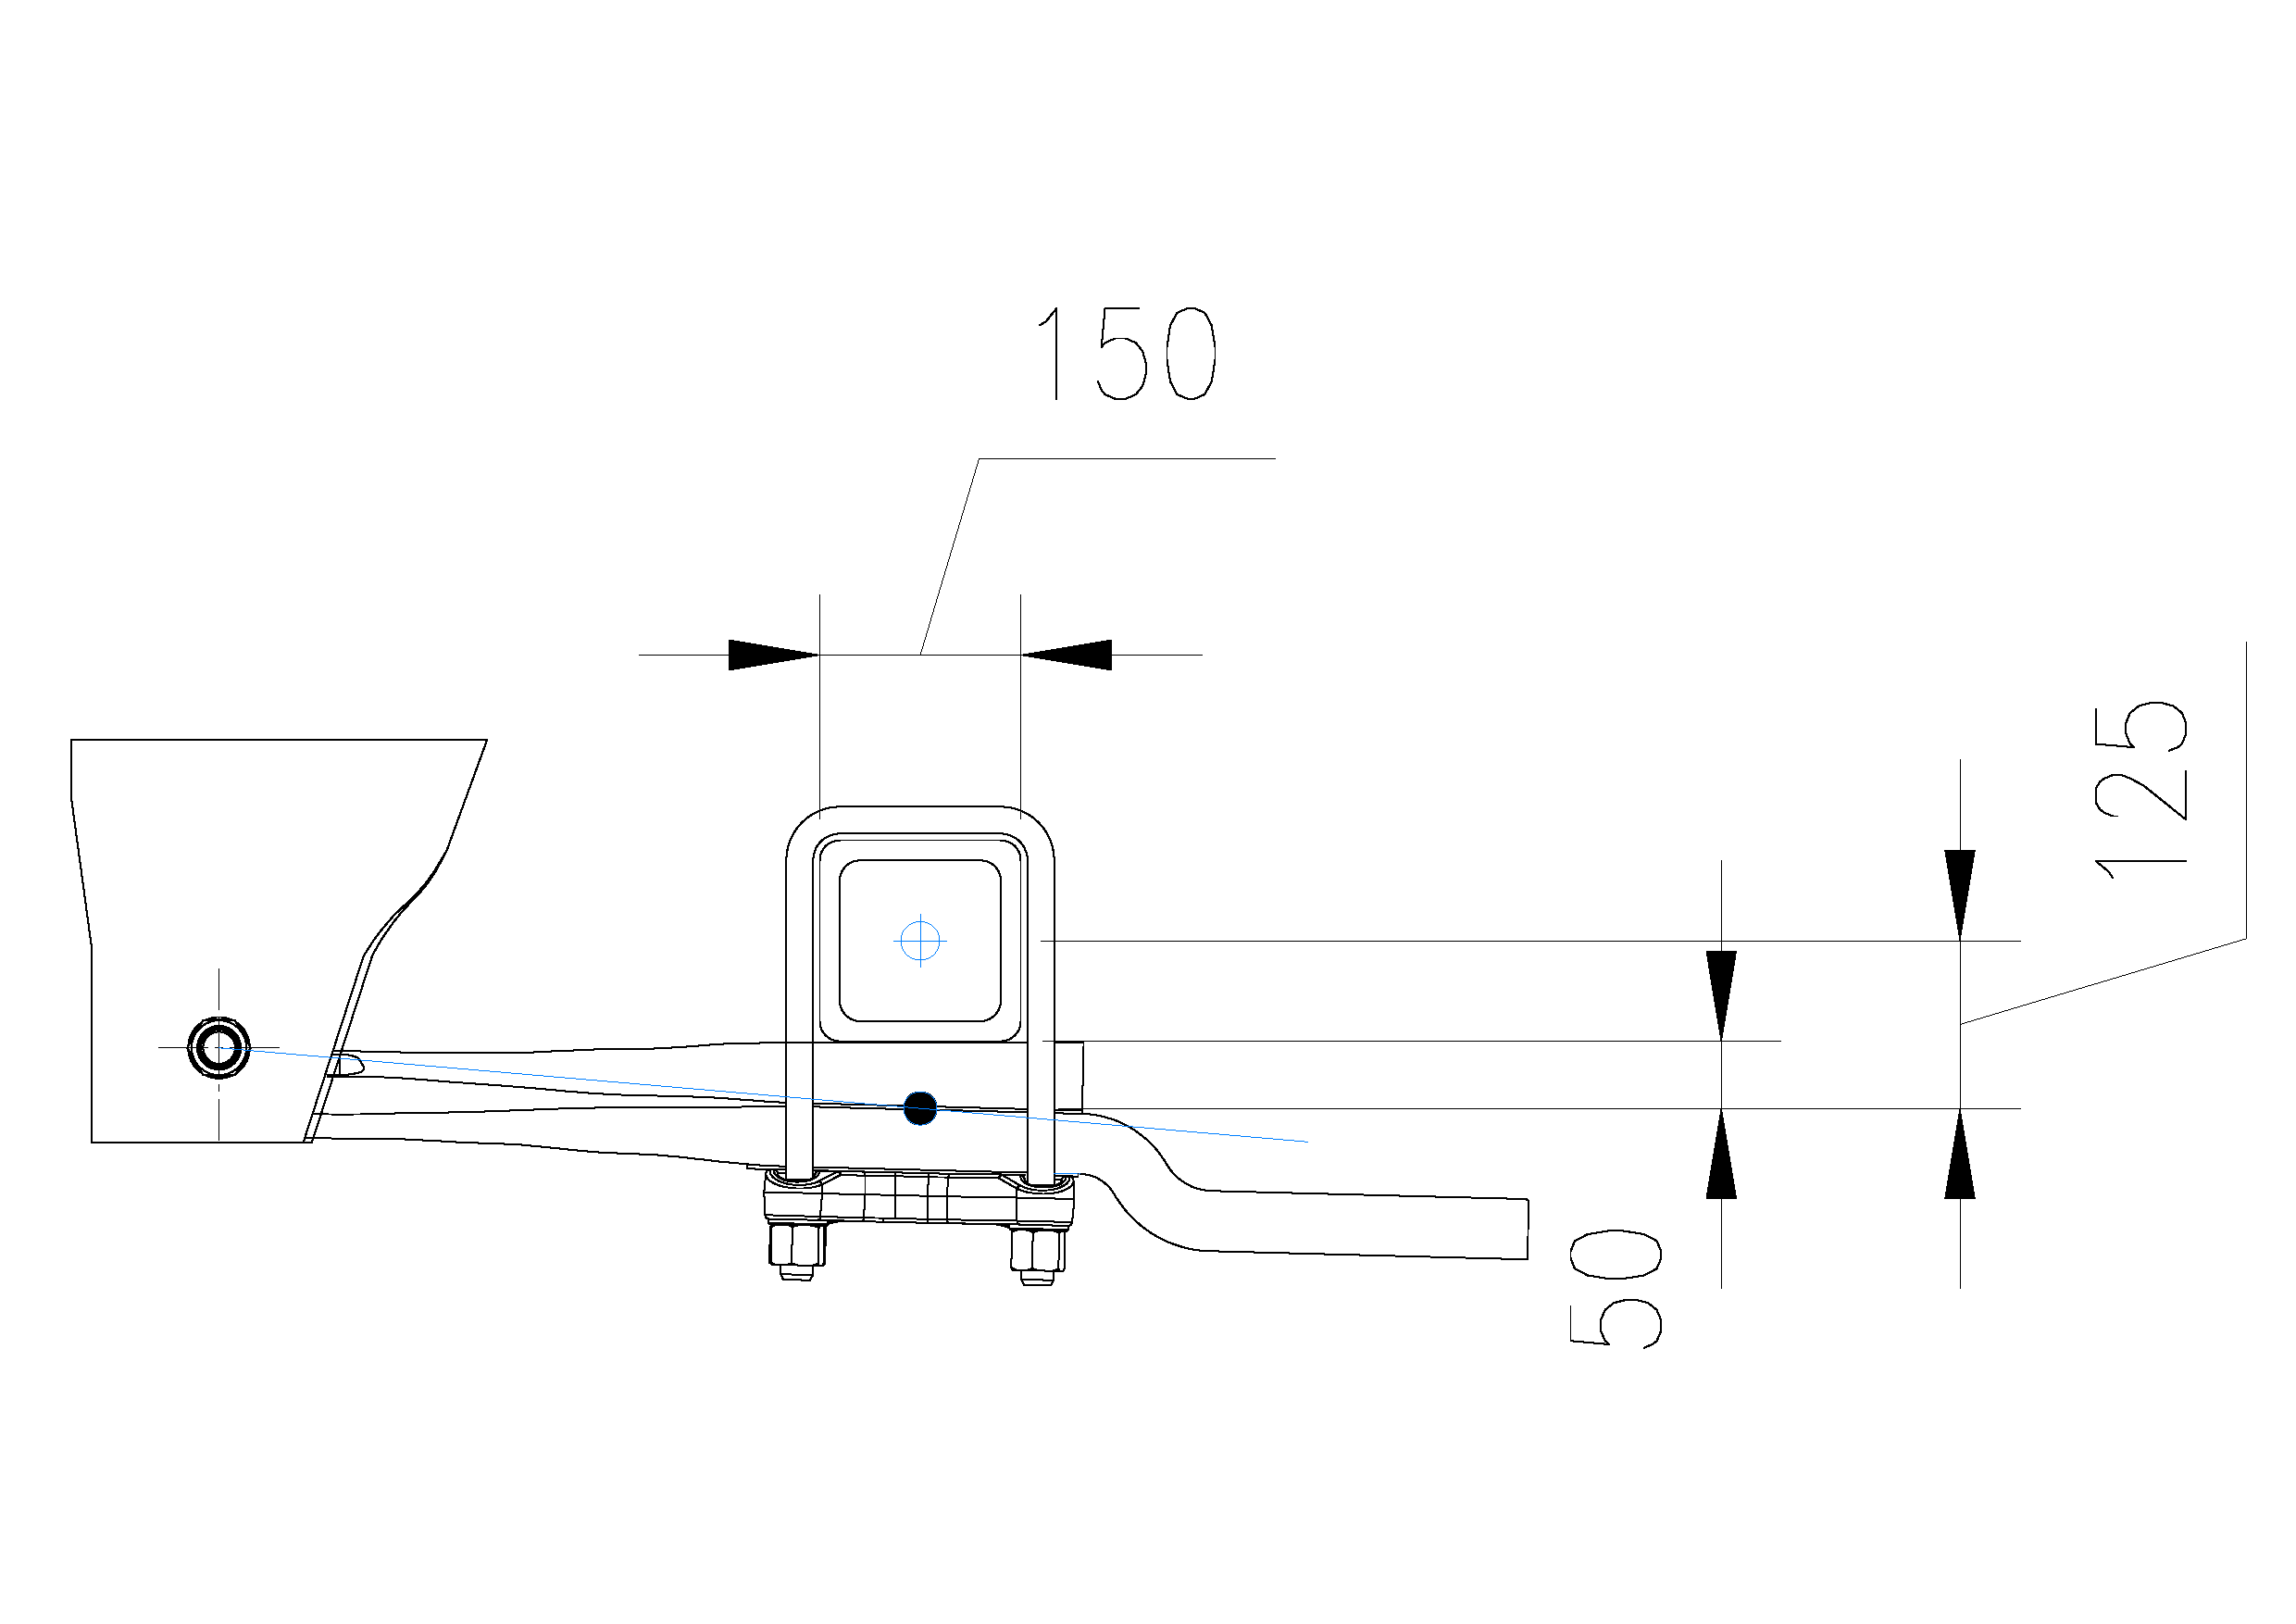
\includegraphics[width=1\textwidth]{fig/parameter-selection_roll-centre-height_underslung}
		\caption{Underslung (-125~mm)}
	\end{subfigure}

	\caption{Roll centre height estimates for trailing arm suspension}
	\label{figure:roll-centre-height-estimates-for-trailing-arm-suspension}
\end{figure*}
%----------------------------------------------
%      FIGURE
%----------------------------------------------

It is desirable from a stability perspective that the roll centre height be raised as high as possible. This is made possible with track bars as noted by Winkler et al. Thus, it was assumed with the use of additional lateral restraints such as a track bar that the maximum height of the roll centre above the trailing arm suspension could reach up to 200~mm.

The suspension used for baseline drive axle tandem bogie is of the A-frame type which  is laterally constrained on the chassis, leading to a high roll centre height of 400~mm above the wheel centre height. An illustration of this type of suspension is included from a Volvo data sheet for the Volvo RADD-GR \cite{VolvoTruckCorporation2012} suspension in Figure~\ref{figure:volvo-radd-gr-rear-axle-installation}.

%----------------------------------------------
%      FIGURE
%----------------------------------------------
\begin{figure}[H]
	\centering
	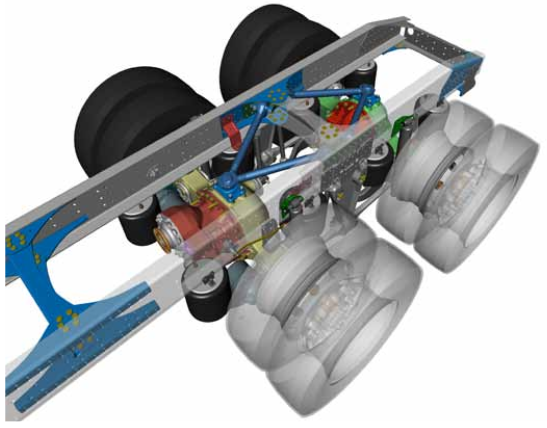
\includegraphics[width=0.5\textwidth]{fig/volvo_radd-gr-bogie-drive-axle-suspension}
	\caption{Volvo RADD-GR rear axle installation}
	\label{figure:volvo-radd-gr-rear-axle-installation}
\end{figure}
%----------------------------------------------
%      FIGURE
%----------------------------------------------

The baseline value of 400~mm was assumed as the maximum height, while the minimum roll centre height was assumed to be the same as for the trailer axles to evaluate the performance with various drive axle suspension designs.

The roll centre height of the steel steer axle suspension is governed by the geometry of the leaf springs as shown by the graphical estimation in Figure~\ref{figure:estimate-of-roll-centre-heights-for-typical-suspension-configurations}. The TERNZ SRT calculator \cite{TERNZTransportResearch} uses a roll centre height of 20~mm below the wheel centre for generic suspensions which was assumed as the minimum. A reasonable maximum was assumed to be 100~mm above the axle centre. The roll centre heights for front air suspension are typically near the axle centre (evident from \gls{oem} data) which was deemed to be representative of both front air and steel suspension designs.

%----------------------------------------------
%      TABLE - UPDATED TO NEW RANGES
%----------------------------------------------
\begin{table}[H]
	\centering\footnotesize
	\begin{threeparttable}

		\begin{tabulary}{\textwidth}{lccc}
			\toprule
			\textbf{Axle} & \textbf{Baseline (mm)\tnote{1}} & \textbf{Min. (mm)} & \textbf{Max. (mm)} \\
			\midrule
             Steer & +21    & -20   & +100 \\
             Drive & +400   & -125  & +400 \\
             Trailer & +114   & -125  & +200 \\
			\bottomrule
		\end{tabulary}

		\caption{Parameter range - roll centre height}
		\label{table:parameter-range-roll-centre-height}

		\begin{tablenotes}
			\item[1] Roll centre height is reported relative to the wheel centre height
		\end{tablenotes}

	\end{threeparttable}
\end{table}
%----------------------------------------------
%      TABLE
%----------------------------------------------

%      SUBSECTION
%----------------------------------------------
\section{Tyre Parameter Limits}\label{section:pr-tyre-properties}

Tyre data is well protected by \glspl{oem} and they are often not willing to disclose measured tyre test data. \gls{pbs} assessments are currently performed using conservative tyre data for lateral tyre force as extracted from \cite{Fancher1981}. This data is from 1981 and modern tyres are expected to have improved properties with advances in material and construction. The use of conservative data aligns with the NTC requirements that worst-case tyre data be used in the absence of measured data for the tyres in question \cite{NationalTransportCommission2008}.

Historically, both bias and radial ply tyres have been used on commercial heavy vehicles. However heavy trucks have been phasing out bias ply in favour of radial ply tyres since 1984 as mentioned by Ervin et al. \cite{Ervin1986}. All modern heavy commercial vehicles use radial ply tyres and hence the mechanical properties of bias ply tyres were not considered.

%      SUBSECTION
%----------------------------------------------
\subsection{Effective Rolling Radius}\label{section:pr-effective-rolling-radius}

The rolling radius is influenced by a multitude of operational factors such as the state of tyre wear, inflation pressure and speed. The effective rolling radius can be estimated from the unloaded tyre radius according to Genta \cite{Giancarlo1997} as 98\% of the unladen tyre radius.

The effective rolling radius for the baseline tyre models was calculated from the Michelin data book \cite{Michelin} using the supplied rolling circumference for each tyre. The effective rolling radius as a percentage of the unladen radius was calculated and it is shown in Table~\ref{table:effective-rolling-radius-of-baseline-tyre-models} that it is approximately 95\% of the unladen radius, with the 445/65 R22.5 tyre model having the lowest ratio of 94.5\%.

%----------------------------------------------
%      TABLE - UPDATED TO NEW RANGES
%----------------------------------------------
\begin{table}[H]
	\centering\footnotesize
	\begin{threeparttable}

		\begin{tabulary}{\textwidth}{lccc}
			\toprule
    \textbf{Tyre} & \textbf{Unladen radius (mm)} & \textbf{Effective rolling radius (mm)} & \textbf{\% of unladen radius} \\

			\midrule
    445/65 R22.5 & 587   & 555   & 94.5\% \\
    315/80 R22.5 & 548   & 522   & 95.3\% \\
    285/70 R19.5 & 456   & 434   & 95.2\% \\
			\bottomrule
		\end{tabulary}

		\caption{Effective rolling radius of baseline tyre models}
		\label{table:effective-rolling-radius-of-baseline-tyre-models}

		%\begin{tablenotes}
		%\item[1] %\tnote{1}
		%\end{tablenotes}

	\end{threeparttable}
\end{table}
%----------------------------------------------
%      TABLE
%----------------------------------------------

Accounting for various operating conditions and considering the effective rolling ratios of the baseline combinations, it was assumed that the effective rolling radius could vary from 94\% to 98\% of the baseline unladen radius. The resulting range of effective rolling radii for each tyre is summarised in Table~\ref{table:pr-tyre-effective-rolling-radius}.

%----------------------------------------------
%      TABLE - UPDATED TO NEW RANGES
%----------------------------------------------
\begin{table}[H]
	\centering\footnotesize
	\begin{threeparttable}

		\begin{tabulary}{\textwidth}{lccc}
			\toprule
            \textbf{Tyre} & \textbf{Baseline (mm)} & \textbf{Min. (mm)} & \textbf{Max. (mm)} \\
			\midrule
            445/65 R22.5 & 555   & 552   & 575 \\
            315/80 R22.5 & 522   & 515   & 537 \\
            285/70 R19.5 & 434   & 429   & 447 \\
			\bottomrule
		\end{tabulary}

		\caption{Parameter range - tyre effective rolling radius}
		\label{table:pr-tyre-effective-rolling-radius}

		%\begin{tablenotes}
		%\item[1] %\tnote{1}
		%\end{tablenotes}

	\end{threeparttable}
\end{table}
%----------------------------------------------
%      TABLE
%----------------------------------------------

%      SUBSECTION
%----------------------------------------------
\subsection{Unloaded Radius}\label{section:pr-unloaded-radius}

Data collected from tyre manufacturer data books (Bridgestone \cite{Bridgestone2015}, Goodyear \cite{Goodyear} and Michelin \cite{Michelin}) and summarised in Tables~\ref{table:spring-rate-approximation-for-445-65R22.5-tyres}~to~\ref{table:spring-rate-approximation-for-285/70 R19.5-tyres} in Appendix~\ref{section:tyre-spring-rate} were consulted to determine the variation in unloaded radii between manufacturers. The range of unloaded radii evaluated is summarised in Table~\ref{table:pr-tyre-unloaded-radius}.

%----------------------------------------------
%      TABLE - UPDATED TO NEW RANGES
%----------------------------------------------
\begin{table}[H]
	\centering\footnotesize
	\begin{threeparttable}

		\begin{tabulary}{\textwidth}{lccc}
			\toprule
			\textbf{Tyre} & \textbf{Baseline (mm)} & \textbf{Min. (mm)} & \textbf{Max. (mm)} \\
			\midrule
            445/65 R22.5 & 587   & 575   & 589 \\
            315/80 R22.5 & 548   & 538   & 550 \\
			285/70 R19.5 & 456   & 448   & 456 \\
			\bottomrule
		\end{tabulary}

		\caption{Parameter range - tyre unloaded radius}
		\label{table:pr-tyre-unloaded-radius}

		%\begin{tablenotes}
		%\item[1] %\tnote{1}
		%\end{tablenotes}

	\end{threeparttable}
\end{table}
%----------------------------------------------
%      TABLE
%----------------------------------------------

%      SUBSECTION
%----------------------------------------------
\subsection{Tyre Spring Rate}\label{section:pr-tyre-spring-rate}

The vertical spring rate of each tyre model was calculated from the given axle load, considering the difference between the unladen and laden radius, the spring of the tyre was estimated assuming linear behaviour and using Equation~\ref{equation:hookes-law} (Hooke's law).

%----------------------------------------------
%      EQUATION
%----------------------------------------------
\begin{align}
	\label{equation:hookes-law}
	\gls{tyrespringrate}=\frac{\gls{fz}}{\Delta{}x}
\end{align}

Where:

\gls{tyrespringrate} = Tyre spring rate (N/mm)

\gls{fz} = Vertical tyre load (N)

\gls{deltax} = Tyre deflection (mm)

%----------------------------------------------
%      EQUATION
%----------------------------------------------

Tyre spring rates were calculated from the data from Bridgestone, Goodyear and Michelin \cite{Bridgestone2015,Goodyear,Michelin} for dual and single tyre arrangements at various pressures and axle loads. Tables~\ref{table:spring-rate-approximation-for-445-65R22.5-tyres}~to~\ref{table:spring-rate-approximation-for-285/70 R19.5-tyres} in Appendix~\ref{section:tyre-spring-rate} include the calculated tyre spring rates. The resulting range of tyre spring rates evaluated is summarised in Table~\ref{table:parameter-range-vertical-tyre-stiffness}.

%----------------------------------------------
%     TABLE - UPDATED TO NEW RANGES
%----------------------------------------------
\begin{table}[H]
	\centering\footnotesize
	\begin{threeparttable}

		\begin{tabulary}{\textwidth}{lccc}
			\toprule
			\textbf{Tyre} & \textbf{Baseline (N/mm)} & \textbf{Min. (N/mm)} & \textbf{Max (N/mm)} \\

			\midrule
             445/65 R22.5 & 1193  & 773   & 1237 \\
             315/80 R22.5 & 987   & 565   & 1169 \\
             285/70 R19.5 & 801   & 473   & 901 \\		

			\bottomrule
		\end{tabulary}

		\caption{Parameter range - tyre spring rate}
		\label{table:parameter-range-vertical-tyre-stiffness}

		%\begin{tablenotes}
		%\item[1] %\tnote{1}
		%\end{tablenotes}

	\end{threeparttable}
\end{table}
%----------------------------------------------
%      TABLE
%----------------------------------------------

\subsection{Wheel and Tyre Assembly Spin Moment of Inertia}\label{section:pr-tyre-spin-moment-of-inertia}

Spin inertias for wheel and tyre assemblies were derived as 10 kg.m\sstw{} for 19.5" wheels and 12 kg.m\sstw{} for 22.5" wheels by de Saxe \cite{DeSaxe2012} from UMTRI data \cite{Winkler1995}, \cite{Winkler1983}. This correlates well with the \trucksim{} database which has values of 13 kg.m\sstw{} (\textit{2000~kg rating, 425 mm Radius (Drive)}) to 28 kg.m\sstw{} (\textit{SAE Widebase, 4750~kg})  for truck tyres. 

It was assumed that the above data are for steel rims. Thus, considering aluminium rims (approximately half the weight of a steel rim) and additional weight reductions in modern designs, the minimum spin moment of inertia was calculated with a reduction in wheel assembly mass of 50\%. The evaluated range of wheel and tyre assembly spin moment of inertias is summarised in Table~\ref{table:pr-wheel-assembly-spin-moment-of-inertia}.

%----------------------------------------------
%      TABLE - UPDATED TO NEW RANGES
%----------------------------------------------
\begin{table}[H]
	\centering\footnotesize
	\begin{threeparttable}

		\begin{tabulary}{\textwidth}{lccc}
			\toprule
    \textbf{Tyre} & \textbf{Baseline (kg.m\sstw{})} & \textbf{Min. (kg.m\sstw{})} & \textbf{Max. (kg.m\sstw{})} \\
			\midrule
    285/70 R19.5 & 10    & 6.5   & 13 \\
    315/80 R22.5 & 12    & 7     & 14 \\
    445/65 R22.5 & 28    & 14    & 28 \\
			\bottomrule
		\end{tabulary}

		\caption{Parameter range - wheel and tyre assembly spin moment of inertia}
		\label{table:pr-wheel-assembly-spin-moment-of-inertia}

		%\begin{tablenotes}
		%\item[1] %\tnote{1}
		%\end{tablenotes}

	\end{threeparttable}
\end{table}
%----------------------------------------------
%      TABLE
%----------------------------------------------

\subsection{Tyre Lag (relaxation length)}\label{section:pr-tyre-lag}
Literature defining truck tyre lag (also known as relaxation length) ranges could not be found, however\trucksim{} indicates that reasonable estimates of  tyre lag are as follows:

\begin{itemize}
	\item \gls{lagfx} (longitudinal tyre lag): 1/10 of the tyre radius
	\item \gls{lagfymz} (lateral tyre lag): Twice the tyre radius
\end{itemize}

The NTC standards and vehicle assessment rules for the PBS framework \cite{NationalTransportCommission2008} do not clearly state whether the simulated vehicle performance should include the effects of tyre lag. Thus tyre lag was varied from the recommended value down to values that would effectively simulate zero tyre lag to evaluate the impact of including the effects of tyre lag in the vehicle simulations.

When tyre lag is set to absolute zero, the driver model is unstable. To simulate zero tyre lag (on all but the steer tyres - see footnote \textsuperscript{1} in Table~\ref{table:parameter-range-tyre-lag}) without causing instabilities in the driver model, resulting in erroneous vehicle performance, the following parameters were used.

\begin{itemize}
	\item \gls{lagfx}: remains at approximately 1/10 of the tyre radius
	\item \gls{lagfymz} : reduced to 100~mm
\end{itemize}

The resulting range of tyre lag values are presented in Table~\ref{table:parameter-range-tyre-lag}.

%----------------------------------------------
%     TABLE - UPDATED TO NEW RANGES
%----------------------------------------------
\begin{table}[H]
	\centering\footnotesize
	\begin{threeparttable}

		\begin{tabulary}{\textwidth}{lccc}
			\toprule
			\textbf{Tyre} & \textbf{Baseline (mm / mm)} & \textbf{Min. (mm / mm)} & \textbf{Max. (mm / mm)} \\
			\midrule
			445/65 R22.5 & 55 / 1100 & 55 / 100 & 55 / 1100 \\
			315/80 R22.5\tnote{1} & 50 / 1000 & 50 / 100 & 50 / 1000 \\
			285/70 R19.5 & 45 / 900 & 45 / 100 & 45 / 900 \\
			\bottomrule
		\end{tabulary}

		\caption{Parameter range - tyre lag (\gls{lagfx} / \gls{lagfymz})}
		\label{table:parameter-range-tyre-lag}

		\begin{tablenotes}
			\item[1] The steer tyre lag is set to 50/1 to prevent instabilities with the driver model. Lag response in the steer tyre causes the driver to overcompensate for the lagged response after a steering input, resulting in instability.
		\end{tablenotes}

	\end{threeparttable}
\end{table}
%----------------------------------------------
%      TABLE
%----------------------------------------------

\subsection{Tyre Cornering Stiffness}\label{section:pr-tyre-cornering-stiffness}

Cornering stiffness tyre data is not readily supplied by manufacturers and could not be used to determine the possible range of tyre data. Conservative tyre models sourced from measured tyre performance provided by \gls{umtri} in studies performed by Fancher \cite{Fancher1981} and Bogard et al. \cite{Bogard1991} are generally used in PBS assessments in South Africa. These same tyre models were used for the baseline combinations.

Fancher et al. \cite{Fancher1986} measured cornering stiffness at rated load for a range of tyres and measured that tyre wear of 1/3 of the tread depth can yield an increase in cornering stiffness of approximately 0.04. This measured data was compared with the cornering stiffness of the baseline combinations to gauge a range of cornering stiffness that should be considered (including the effect of increased cornering stiffness with tyre wear).

The steer, drive and trailer tyres were evaluated separately to provide insight into how using tyres of varying cornering stiffness on the same combination could influence behaviour as well as yield insight into the sensitivity of vehicle performance to the cornering stiffness of the tyres. Situations like this can occur when worn tyres are rotated from the prime mover to the trailer or retreads of unknown cornering stiffness properties are used.

The cornering stiffness was calculated within the linear region of each tyre for the same vertical loading at which the tyres were tested by Fancher et al. of 26879~N (6040 Lbs). The cornering stiffness was then normalised with the vertical tyre load according to Equation~\ref{equation:cornering-coefficient} to determine the cornering coefficient which could then be compared to the data provided by Fancher et al.

%----------------------------------------------
%      EQUATION
%----------------------------------------------
\begin{align}
	\label{equation:cornering-coefficient}
	C_{c} = \frac{C_{\alpha{}}}{F_z}
\end{align}

Where:

\gls{ccornering} = Cornering coefficient (\degree{}\textsuperscript{-1})

\gls{calpha} = Cornering stiffness (N/\degree{})

\gls{fz} = Vertical tyre load (N)

%----------------------------------------------
%      EQUATION
%----------------------------------------------

The variation for the cornering stiffness values are summarised in Table~\ref{table:cornering-stiffness-variation}. The baseline cornering stiffness values are conservative in relation to the cornering stiffness values measured by Fancher et al. \cite{Fancher1986}. This is in-line with the requirements of the NTC for PBS assessments which state \cite{NationalTransportCommission2008} that if no tyre data is available, conservative worst-case tyre data must be used.

Using the variations as a guideline, a conservative range of cornering stiffness values relative to the baseline models were evaluated as per Table~\ref{table:pr-tyre-cornering-stiffness}. 

%----------------------------------------------
%      TABLE - UPDATED TO NEW RANGES
%----------------------------------------------
\begin{table}[H]
	\centering\footnotesize
	\begin{threeparttable}

		\begin{tabulary}{\textwidth}{lcccccCC}
			\toprule
			\textbf{Tyre} & \textbf{Load} & \boldmath{}\textbf{$C_\alpha{}$ (N/\degree{})}\unboldmath{} & \boldmath{}\textbf{$C_c$ (/\degree{})}\unboldmath{} & \boldmath{}\textbf{Min. $C_c$ (/\degree{})\tnote{1}}\unboldmath{} & \boldmath{}\textbf{Max. $C_c$ (/\degree{})\tnote{1} \textsuperscript{,} \tnote{2}}\unboldmath{} & \textbf{Min.\tnote{3}} & \textbf{Max.\tnote{3}} \\
			\midrule
			445/65 & 26879 & 2886  & 0.1074 & 0.1121 & 0.1861 & 104\% & 173\% \\
			315/80 & 26879 & 2775  & 0.1033 & 0.1121 & 0.1861 & 109\% & 180\% \\
			285/70 & 26879 & 3115  & 0.1159 & 0.1121 & 0.1861 & 97\%  & 161\% \\
			\bottomrule
		\end{tabulary}

		\caption{Cornering stiffness variation}
		\label{table:cornering-stiffness-variation}

		\begin{tablenotes}
		\item[1] Including the effects of tyre wear (additional 0.04 to the cornering coefficient)
		\item[2] Fancher et al. \cite{Fancher1986}
		\item[3] Variation relative to the baseline cornering coefficient
		\end{tablenotes}

	\end{threeparttable}
\end{table}
%----------------------------------------------
%      TABLE
%----------------------------------------------

%----------------------------------------------
%      TABLE - UPDATED TO NEW RANGES
%----------------------------------------------
\begin{table}[H]
	\centering\footnotesize
	\begin{threeparttable}

		\begin{tabulary}{\textwidth}{lccc}
			\toprule
			\textbf{Tyre} & \textbf{Baseline\tnote{1}} & \textbf{Min.} & \textbf{Max.} \\
			\midrule
			445/65 R22.5 & 100\% & 100\% & 173\% \\
			315/80 R22.5 & 100\% & 100\% & 180\% \\
			285/70 R19.5 & 100\% & 97\%  & 161\% \\

			\bottomrule
		\end{tabulary}

		\caption{Parameter range - tyre cornering stiffness}
		\label{table:pr-tyre-cornering-stiffness}

		\begin{tablenotes}
		\item[1] The cornering stiffness is reported as a percentage of the baseline value
		\end{tablenotes}

	\end{threeparttable}
\end{table}
%----------------------------------------------
%      TABLE
%----------------------------------------------

Scaling the baseline tyre data causes the coefficient of friction for the data to be skewed to unrealistic values and this results in the tyre lateral force saturating at unrealistically low slip angles. To prevent this, the baseline tyre models were converted to equivalent Pacejka '89 models \cite{Bakker1989}. The Pacejka '89 models were then scaled by manipulating the maximum cornering stiffness shape factor ($a3$) within the tyre cornering stiffness range in Table~\ref{table:pr-tyre-cornering-stiffness} to generate more realistically scaled tyre curves.

\subsection{Dual Tyre Spacing}\label{section:pr-dual-tyre-spacing}

Minimum dual tyre spacing is quoted by tyre \glspl{oem} to ensure that the tyres do not touch during operation which would severely reduce the tyre life as well as become a fire risk.

Minimum dual tyre spacing for the 315/80 R22.5 and 285/70 R19.5 dual tyre assemblies were found in the \gls{oem} data books from Michelin, Goodyear and Bridgestone \cite{Michelin,Goodyear,Bridgestone2015} and are reported in Table~\ref{table:minimum-dual-tyre-spacings}. In general the minimum spacings are similar, with a maximum difference of 4~mm between \glspl{oem}.

The dual spacing of the baseline vehicles was modelled on the Michelin data, which is consistently the minimum between all manufactures. Thus, assuming that a standard 5~mm plate can be used as a spacer between rims to account for various tyre models, the baseline dual tyre spacing was varied from the baseline value to a maximum of 5~mm additional spacing as per Table~\ref{table:pr-dual-tyre-spacing}.

%----------------------------------------------
%      TABLE - UPDATED TO NEW RANGES
%----------------------------------------------
\begin{table}[H]
	\centering\footnotesize
	\begin{threeparttable}

		\begin{tabulary}{\textwidth}{lccc}
			\toprule
            \textbf{Tyres} & \textbf{Michelin} & \textbf{Goodyear} & \textbf{Bridgestone} \\
			\midrule
               
            315/80 R22.5 & 350   & 351   & 350.5 \\
            285/70 R19.5 & 314   & 318   & 317.5 \\
			
            \bottomrule
		\end{tabulary}

		\caption{Minimum dual tyre spacings}
		\label{table:minimum-dual-tyre-spacings}

		%\begin{tablenotes}
		%\item[1] \tnote{1}
		%\end{tablenotes}

	\end{threeparttable}
\end{table}
%----------------------------------------------
%      TABLE
%----------------------------------------------

%----------------------------------------------
%      TABLE - UPDATED TO NEW RANGES
%----------------------------------------------
\begin{table}[H]
	\centering\footnotesize
	\begin{threeparttable}

		\begin{tabulary}{\textwidth}{lccc}
			\toprule
            \textbf{Tyres} & \textbf{Baseline (mm)} & \textbf{Minimum (mm)} & \textbf{Maximum (mm)} \\
			\midrule  
    		
            315/80 R22.5 & 350   & 350   & 355 \\
            285/70 R19.5 & 314   & 314   & 319 \\
			
            \bottomrule
		\end{tabulary}

		\caption{Parameter range - dual tyre spacing}
		\label{table:pr-dual-tyre-spacing}

		%\begin{tablenotes}
		%\item[1] \tnote{1}
		%\end{tablenotes}

	\end{threeparttable}
\end{table}
%----------------------------------------------
%      TABLE
%----------------------------------------------